% PM-001 (FTC Team 207): backspin entry of POLLEN into the up-facing HIVE CELL.
% Assembled paper. The section files in sections/ hold the derivations; this file holds the
% preamble, the provenance macros, the abstract, the introduction, the notation table, the
% figures, the limitations and the references.
% The code in src/*.py is the source of truth for every equation in this paper.
\documentclass[11pt]{article}

\usepackage[margin=1in]{geometry}
\usepackage{amsmath}
\usepackage{amssymb}
\usepackage{bm}
\usepackage{booktabs}
\usepackage{graphicx}
\usepackage[hidelinks]{hyperref}

\graphicspath{{../figures/}}

% ---------------------------------------------------------------------------------------------
% Provenance tags. Every number in the paper carries exactly one of them.
%   \confirmed  [C]  official CAD or competition manual
%   \assumed    [A]  assumed or swept value
%   \derived    [D]  derived from other values by arithmetic or geometry
%   \predicted  [P]  model output
%   \userval    [U]  value given by the team
% The tags work in text and in math mode.
\makeatletter
\DeclareRobustCommand{\provtag}[1]{%
  \ifmmode\text{\provtag@text{#1}}\else\provtag@text{#1}\fi}
\newcommand{\provtag@text}[1]{%
  \textsuperscript{\textsf{\upshape\scriptsize\color@grey[#1]}}}
% Grey without the xcolor package: use the PDF fill-colour operator through \pdfliteral when it
% exists, otherwise print the tag in black.
\ifx\pdfliteral\@undefined
  \newcommand{\color@grey}[1]{#1}
\else
  \newcommand{\color@grey}[1]{\pdfliteral{0.45 g}#1\pdfliteral{0 g}}
\fi
\makeatother
\DeclareRobustCommand{\confirmed}{\provtag{C}}
\DeclareRobustCommand{\assumed}{\provtag{A}}
\DeclareRobustCommand{\derived}{\provtag{D}}
\DeclareRobustCommand{\predicted}{\provtag{P}}
\DeclareRobustCommand{\userval}{\provtag{U}}

% Bold vector, upright unit, monospace code name.
\newcommand{\vect}[1]{\bm{#1}}
% \unit{m/s}: upright text. Directly after an inline-math number ("$3$\unit{m}") it inserts the
% thin space itself; after "\," or a space it adds nothing, so "$3$\,\unit{m}" and "(\unit{m})"
% print with one thin space and with none respectively.
\DeclareRobustCommand{\unit}[1]{%
  \ifmmode\text{\upshape #1}%
  \else
    \ifnum\lastnodetype=10 \,\fi
    \textup{#1}%
  \fi}
% Inside \code an escaped underscore allows a line break after it, so long function and
% file names do not run into the margin.
\DeclareRobustCommand{\code}[1]{{\def\_{\textunderscore\allowbreak}\texttt{#1}}}

% Paragraphs with long unbreakable names may set a loose line rather than run into the margin.
\emergencystretch=6em

\title{Backspin Entry of POLLEN into the HIVE CELL:\\ Model Equations and Derivations}
\author{FTC Team 207 Critical Mass, PM-001}
\date{\today}

\begin{document}
\maketitle

\begin{abstract}
\noindent
We derive, step by step, the equations of a model that asks whether a single powered
98\,\unit{mm}\userval{} flywheel, with a fixed curved hood or an optional passive upper roller, can
put enough backspin on POLLEN (a perforated polyethylene ball of diameter about
71\,\unit{mm}\confirmed{} and mass about 25\,\unit{g}\assumed{} from the vendor listing \cite{andymark}) to make it enter the upward-facing
CELL of the pivoting HIVE from the unfavourable side, where the CELL roof stands between the robot
and the mouth. The model has five parts: the HIVE cross-section and an exact clean-entry test, a
flight model with drag, a capped Magnus lift and spin decay, a launcher contact model, a rigid-body
rim and interior collision law, and a robustness layer that turns entry windows into a shooter
specification. Every equation matches what the code in \code{src/} computes.

\emph{Every result in this paper is a model prediction.} No aerodynamic or contact property of
POLLEN has been measured: drag, spin lift, spin decay, restitution and friction all take assumed
ranges based on pickleball and smooth-sphere literature, which are not POLLEN measurements and are
not proven bounds. Within those ranges the model predicts that a clean far-side entry is physically
possible, but only if the shooter holds its exit speed and elevation to a tight tolerance after the
wheel speed has been tuned on the field. With the nominal coefficients and the
$30^\circ$\confirmed{} tilt, the largest all-clean box is about $\pm0.075$\,\unit{m/s}\predicted{}
by $\pm0.15^\circ$\predicted{} with backspin (spin parameter $S=0.5$\assumed{} or $1.0$\assumed)
and $\pm0.05$\,\unit{m/s}\predicted{} by $\pm0.10^\circ$\predicted{} for the no-spin twin
($S=0$\assumed). These are requirements on the shooter, not a measured repeatability.
% CHECK 2026-10-31: data/_spec_cache *_nominal.npz, unfav_t30, 120 (h, d) rows, best_square: S=0 k*=3
% in 89 rows (none above 3), S=0.5 k*=4 in 4 rows, S=1.0 k*=4 in 10 rows, no k*=5 (spec_nominal.csv
% agrees). Other single conditions differ (S=0 with high Cd reaches k*=4), so the nominal set is named.
Backspin shifts the clean window to other speeds and angles rather than being required for it:
no-spin shots have clean windows of their own, and more spin is not always better, because the lift
coefficient saturates in this model and backspin can lower retention after a contact.
Over a field grid of $144$\derived{} scored release poses, backspin never has a clearly higher
clean-entry chance than a no-spin twin scored on the same simulated shots. Tuned to whichever of
the three assumed lift sets (low, nominal, high) is true, it is level with the twin
(unfavourable-side medians $34.4$\predicted{} to $35.7\,\%$\predicted{} against
$35.2\,\%$\predicted); one setting for an unknown lift is lower.
\end{abstract}

\tableofcontents

% =============================================================================================
\section{Introduction}
\label{sec:intro}

\paragraph{The game question.}
In the FTC BIOBUZZ game the centre HIVE is a rigid beam with a box-shaped CELL at each end. It
rotates about a horizontal pivot axis between two stable tipped positions, and only one CELL faces
upward at a time. Teams LAUNCH POLLEN into that upward-facing CELL to make the HIVE tip
\cite{manual,gameres}. From one side of the field the CELL mouth faces the robot (the
\emph{favourable} side). From the other side the CELL roof is between the robot and the mouth (the
\emph{unfavourable} side), and an ordinary lob has to fall very steeply to get in.

The team has seen backspinning POLLEN behave in a way that seemed to help on the unfavourable
side. The proposed mechanism is a high arc with strong backspin whose path is reshaped by the
Magnus force. One point needs care from the start: at the apex of the arc only the vertical
velocity is zero, $v_z=0$; the ball keeps its horizontal speed, and spin gives it no sudden new
push there. The Magnus force acts during the whole flight and depends on the spin and the
air-relative velocity together. Whether it helps is therefore a trajectory-and-clearance
calculation, which is what this paper sets up.

\paragraph{Two hypotheses.}
The team reported two effects, and we keep them apart:
\begin{itemize}
  \item[(A)] \textbf{Air-only clean entry.} A backspinning ball follows a Magnus-shaped flight that
    passes over the roof and enters the CELL without touching any part of the HIVE.
  \item[(B)] \textbf{Magnus flight plus a rim contact.} The ball flies a Magnus-shaped path, touches
    the CELL rim or interior, and the spin-dependent collision redirects it into the CELL (or out of
    it).
\end{itemize}
Neither hypothesis is assumed to be true. Sections~\ref{sec:geometry}--\ref{sec:flight} and
\ref{sec:robust_spec} test (A); Section~\ref{sec:contact} tests (B); Section~\ref{sec:launcher}
asks which exit states a single powered wheel can actually produce. Section~\ref{sec:svt} compares
the clean-entry chance of backspin with that of a no-spin twin over the whole field.

\paragraph{How to read the numbers.}
Every number carries one grey tag that says where it comes from:
\begin{center}
\begin{tabular}{@{}lll@{}}
  \toprule
  Tag & Macro & Meaning \\
  \midrule
  \confirmed & \texttt{\char92 confirmed} & official CAD or competition manual \\
  \assumed   & \texttt{\char92 assumed}   & assumed, chosen or swept value \\
  \derived   & \texttt{\char92 derived}   & computed from other values by arithmetic or geometry \\
  \predicted & \texttt{\char92 predicted} & output of the model (a prediction, not a measurement) \\
  \userval   & \texttt{\char92 userval}   & value given by the team \\
  \bottomrule
\end{tabular}
\end{center}
The aerodynamic and contact ranges are based on pickleball and smooth-sphere work
\cite{emond2024,steyn2025,vanwyk2026}, collected in the project literature synthesis
\cite{litsynth}; the launcher model starts from the flywheel analysis of \cite{brettle}.
Every worked example was computed by running the repository code. The code is the source of
truth: where a project document disagrees with the code, the text follows the code and the
source file carries a comment recording the difference. Aerodynamic parameter ranges come from
\code{research/params\_lit.json}, the current default; the older first-pass set
\code{data/aero\_params.json} is named only where a result was produced with it.

\paragraph{What the paper does not claim.}
It does not claim that more backspin is always better, that a dual-powered-wheel shooter is
needed, or that a single successful shot shows repeatability. The literature coefficients for
pickleballs and smooth spheres are used only as assumed ranges, not as POLLEN values.

% ---------------------------------------------------------------------------------------------
\subsection*{Notation}
\addcontentsline{toc}{subsection}{Notation}

Tables~\ref{tab:notation-1}--\ref{tab:notation-4} list each symbol with the meaning it
has where it first appears. Units are SI unless stated. Some letters are reused later with a local
meaning; those reuses are listed below and are always defined again at their first use in the
section concerned.

\begin{table}[p]
\centering
\small
\caption{Notation, part 1 of 4: HIVE geometry and the clean-entry test (Section~\ref{sec:geometry}).}
\label{tab:notation-1}
\begin{tabular}{@{}p{0.24\linewidth}p{0.56\linewidth}p{0.14\linewidth}@{}}
  \toprule
  Symbol & Meaning & Units \\
  \midrule
  $x$ & HIVE-frame horizontal coordinate in the tipping plane, $+x$ toward the audience; origin on the tile below the pivot axis & m \\
  $z$ & HIVE-frame vertical coordinate above the tiles & m \\
  $y$ & coordinate along the pivot axis & m \\
  $\vect{p}=(x,z)$ & point or ball-centre position in the tipping plane & m \\
  $z_p$ & pivot-axis height above the tiles ($1.11633$\confirmed) & m \\
  $u$ & cell-local coordinate along the cell axis, toward the up-CELL mouth & m \\
  $w$ & cell-local coordinate perpendicular to $u$, toward the CELL roof & m \\
  $s$ & lateral coordinate across the CELL opening (zero on the centre plane) & m \\
  $\tau$ & HIVE tilt: angle of the cell axis above horizontal (nominal $30^\circ$\confirmed) & rad (quoted in deg) \\
  $\sigma$ & pose sign, $+1$ for \code{pose\_pos}, $-1$ for \code{pose\_neg} & -- \\
  $\vect{p}_r=(-d,h)$ & release point of the ball centre in the shot frame & m \\
  $d$ & horizontal distance from the release point to the pivot plane $x=0$ & m \\
  $h$ & ball-centre height above the tiles at release & m \\
  $u_M$ & cell-local mouth plane ($0.54508$\confirmed) & m \\
  $u_B$ & cell-local back wall ($0.23952$\confirmed) & m \\
  $w_F$ & cell-local floor, lower lip ($-0.03734$\confirmed) & m \\
  $w_C$ & cell-local ceiling, upper lip; roof underside at the peak ($0.32004$\confirmed) & m \\
  $w_T$ & cell-local roof-top envelope ($0.33325$\confirmed) & m \\
  $L$ & mouth length $w_C-w_F$ ($0.35738$\derived) & m \\
  $\vect{a}_j,\vect{b}_j$ & end points of obstacle segment $j$ & m \\
  $\vect{n}$ & outward unit normal of the mouth, $(\sigma\cos\tau,\ \sin\tau)$ & -- \\
  $\vect{m}$ & unit direction of the mouth line from the lower to the upper lip & -- \\
  $\vect{v}=(v_x,v_z)$ & ball velocity & m/s \\
  $z_{\mathrm{lip}}(\tau)$ & lower-lip height as a function of tilt & m \\
  $\Delta z_{\mathrm{lip}},\ \Delta\tau$ & checklist lip-height tolerance and the resulting tilt tolerance & in; deg \\
  $R$ & POLLEN radius ($0.0355$\confirmed) & m \\
  $\lambda_j^\ast$ & clipped fraction along segment $j$ of the nearest point to $\vect{p}$ & -- \\
  $\vect{q}_j$ & nearest point on segment $j$ to $\vect{p}$ & m \\
  $\delta_j(\vect{p})$ & distance from $\vect{p}$ to segment $j$ & m \\
  $c(\vect{p})$ & clearance: minimum distance to the obstacles minus $R$; contact if and only if $c<0$ & m \\
  $\Delta$ & C-space raster cell size ($1$\,\unit{mm}\assumed) & m \\
  $\mathcal{I}$ & inside region of the CELL (a quadrilateral in $u,w$) & m (region) \\
  $\vect{A},\vect{B}$ & low and high ends of the gate (mouth-plane edge of the inside region) & m \\
  $L_g$ & gate length $L-2R$ ($0.28638$\derived) & m \\
  \bottomrule
\end{tabular}
\end{table}

\begin{table}[p]
\centering
\small
\caption{Notation, part 2 of 4: Section~\ref{sec:geometry}, continued: paths, crossing and descent angle.}
\label{tab:notation-2}
\begin{tabular}{@{}p{0.24\linewidth}p{0.56\linewidth}p{0.14\linewidth}@{}}
  \toprule
  Symbol & Meaning & Units \\
  \midrule
  $v$ & launch speed & m/s \\
  $\theta$ & launch elevation angle & deg \\
  $t$ & time since release & s \\
  $\vect{\Pi}(t)=(\Pi_x,\Pi_z)$ & path shape relative to the release point (translation-invariant without wind) & m \\
  $t_k$ & time of solver sample $k$ & s \\
  $s_g$ & fraction along the gate from $\vect{A}$ ($0$) to $\vect{B}$ ($1$) & -- \\
  $x_g$ & $x$ of the gate point at the sample height & m \\
  $g$ & standard gravity ($9.80665$\confirmed) & m/s\textsuperscript{2} \\
  $v_{z0}$ & initial vertical launch speed & m/s \\
  $c_2,c_1,c_0$ & coefficients of the mouth-line crossing quadratic & m/s\textsuperscript{2}, m/s, m \\
  $t_1,t_2$ & roots of the mouth-line crossing quadratic & s \\
  $\varphi$ & descent angle of the velocity below horizontal, $\operatorname{atan2}(-v_z,v_x)$ & deg \\
  $\varphi_{\mathrm{kin}}$ & kinematic minimum descent angle $90^\circ-\tau$ & deg \\
  $\alpha$ & excess descent angle $\varphi+\tau-90^\circ$ & deg \\
  $\vect{T}=(x_T,z_T)$ & roof top at the mouth, the highest HIVE point & m \\
  $\kappa$ & path curvature under gravity, $g\cos\varphi/|\vect{v}|^2$ & 1/m \\
  $\hat{\vect{e}}_{uw}$ & unit direction of motion in the cell-local frame, $(-\sin\alpha,-\cos\alpha)$ & -- \\
  $w_c$ & cell-local $w$ at which the centre crosses the mouth plane & m \\
  $\lambda$ & distance travelled back along the path from the crossing & m \\
  $\vect{C},\vect{D}$ & upper-lip and lower-lip inner corners $(u_M,w_C)$, $(u_M,w_F)$ & m \\
  $\delta_C,\delta_D$ & distance of the straight path line from the upper and lower lip corner & m \\
  $\varphi_{\mathrm{gate}}$ & minimum descent angle for a clean straight path under the code's gate criterion ($66.33^\circ$\derived{} at $30^\circ$\confirmed{} tilt) & deg \\
  $\varphi_{\mathrm{fit}}$ & stricter both-lips minimum descent angle ($71.46^\circ$\derived{} at $30^\circ$\confirmed{} tilt) & deg \\
  $W_\perp(\alpha)$ & width of the clean straight-path window, measured perpendicular to the path & m \\
  $H_{\max}$ & R105 robot height limit ($0.7366$\confirmed) & m \\
  $\Delta w(s)$ & roof drop for lateral offset $s$ (2D proxy of the pentagon roof) & m \\
  $h_0,h_w,s_{\mathrm{half}}$ & pentagon peak height, side-wall height and half-width used in the roof drop & m \\
  \bottomrule
\end{tabular}
\end{table}

\begin{table}[p]
\centering
\small
\caption{Notation, part 3 of 4: Flight dynamics (Section~\ref{sec:flight}).}
\label{tab:notation-3}
\begin{tabular}{@{}p{0.24\linewidth}p{0.56\linewidth}p{0.14\linewidth}@{}}
  \toprule
  Symbol & Meaning & Units \\
  \midrule
  $x,\,y,\,z;\ \hat{\vect{x}},\hat{\vect{y}},\hat{\vect{z}}$ & world frame: $x$ horizontal toward the target, $y$ sideways, $z$ up; unit vectors & m; unit vectors -- \\
  $\vect{r}$ & ball-centre position & m \\
  $\vect{\omega}$ & spin (angular velocity) vector & rad/s \\
  $\vect{\omega}_0,\ \omega_0$ & launch spin vector; signed launch spin rate (positive = backspin) used by \code{backspin\_omega} & rad/s \\
  $\omega_y$ & $y$ component of spin in the 2D reduction (negative = backspin toward $+x$) & rad/s \\
  $m$ & ball mass & kg \\
  $D=2R$ & ball diameter & m \\
  $\rho$ & air density & kg/m\textsuperscript{3} \\
  $\nu$ & kinematic viscosity of air & m\textsuperscript{2}/s \\
  $A=\pi R^2$ & frontal (cross-sectional) area & m\textsuperscript{2} \\
  $\vect{u}$ & wind velocity & m/s \\
  $\vect{v}_{\mathrm{rel}}=\vect{v}-\vect{u}$ & air-relative velocity & m/s \\
  $\vect{F}_D$ & drag force & N \\
  $\vect{F}_M$ & Magnus force & N \\
  $q$ & dynamic pressure $\tfrac12\rho|\vect{v}_{\mathrm{rel}}|^2$ & Pa \\
  $C_d$ & drag coefficient (constant per run) & -- \\
  $C_L$ & lift (Magnus) coefficient, a function of $S$ & -- \\
  $C_{L,\max}$ & lift-coefficient ceiling & -- \\
  $S$ & spin parameter $|\vect{\omega}|R/|\vect{v}_{\mathrm{rel}}|$ & -- \\
  $S_0$ & spin parameter at launch (signed in \code{feasibility.py}, $>0$ = backspin) & -- \\
  $S_{\mathrm{sat}}=C_{L,\max}/c_1$ & saturation spin parameter above which $C_L$ is capped & -- \\
  $\varepsilon_v$ & regularisation speed ($10^{-6}$\assumed) in $S$ and in the Magnus direction & m/s \\
  $\mathrm{Re}$ & Reynolds number $|\vect{v}_{\mathrm{rel}}|\,2R/\nu$ (diagnostic only) & -- \\
  $\hat{\vect{n}}_M$ & Magnus direction, the unit vector of $\vect{\omega}\times\vect{v}_{\mathrm{rel}}$ & -- \\
  $k$ & spin-decay rate & 1/s \\
  $t_{1/2}$ & spin half-life $\ln2/k$ & s \\
  $v_0$ & launch speed & m/s \\
  $C_M=\beta S$ & spin-down moment coefficient (literature model, not in the code) & -- \\
  $\beta$ & spin-down moment slope (literature model) & -- \\
  $I_b=\alpha mR^2$ & ball moment of inertia & kg\,m\textsuperscript{2} \\
  $k_{\mathrm{torque}}$ & speed-dependent decay rate from the torque model (not implemented) & 1/s \\
  \bottomrule
\end{tabular}
\end{table}

\begin{table}[p]
\centering
\small
\caption{Notation, part 4 of 4: Section~\ref{sec:flight}, continued, and Sections~\ref{sec:launcher}--\ref{sec:robust_spec}.}
\label{tab:notation-4}
\begin{tabular}{@{}p{0.24\linewidth}p{0.56\linewidth}p{0.14\linewidth}@{}}
  \toprule
  Symbol & Meaning & Units \\
  \midrule
  $s_b$ & backspin sign, $-\operatorname{sgn}(\omega_y)$, $+1$ for backspin toward $+x$ & -- \\
  $v_t$ & terminal speed $\sqrt{2mg/(\rho C_d A)}$ & m/s \\
  $a_D,\ a_M$ & drag and Magnus accelerations & m/s\textsuperscript{2} \\
  $a_\perp$ & acceleration normal to the velocity & m/s\textsuperscript{2} \\
  $r_c$ & local radius of curvature of the path & m \\
  $\Delta z_{\mathrm{apex}},\ \Delta x_{\mathrm{land}}$ & apex-height gain and landing-point shift caused by spin, compared with no spin & m (tabulated in cm) \\
  $\vect{y},\ \vect{f},\ \vect{k}_1,\dots,\vect{k}_4$ & generic ODE state, right-hand side, RK4 stages & state units; stages per s \\
  $\vect{a}_1,\vect{a}_2,\vect{a}_3$ & acceleration stages in the position form of RK4 & m/s\textsuperscript{2} \\
  $r_{\mathrm{tol}},\ a_{\mathrm{tol}}$ & relative and absolute tolerances of \code{solve\_ivp} & --; state units \\
  $e_i$ & local error estimate of state component $i$ & state units \\
  $C$ & RK4 global-error constant & m/s\textsuperscript{4} \\
  \midrule
  $n$ & flywheel speed (Section~\ref{sec:launcher}) & rev/min \\
  $\Omega$ & flywheel angular velocity, positive when the wheel surface at the contact moves forward & rad/s \\
  $\Omega_t$ & passive-roller angular velocity, positive when its surface at the contact moves forward & rad/s \\
  $R_w$ & flywheel radius & m \\
  $e$ & coefficient of restitution of a contact (Section~\ref{sec:contact}) & -- \\
  $e_t$ & tangential restitution coefficient & -- \\
  $\mu$ & Coulomb friction coefficient of a contact & -- \\
  $\psi$ & shot azimuth away from the tipping plane (Section~\ref{sec:robust_spec}) & deg or rad \\
  $\hat p$ & estimated success rate $k/n$ from $k$ successes in $n$ shots & -- \\
  \bottomrule
\end{tabular}
\end{table}

\paragraph{Reused letters.}
The alphabet is small, so a few letters change meaning between sections. Each is redefined at its
first use there:
$c_1$ is also the initial slope of the linear-capped lift law (Section~\ref{sec:flight});
$\kappa$ is also the drag constant $\rho A/(2m)$ (\unit{1/m}) of the 2D flight equations;
$\alpha$ is also the moment-of-inertia shape factor in $I_b=\alpha mR^2$ (Sections~\ref{sec:flight}
and \ref{sec:contact});
$\tau$ is also the spin-down torque of the literature model (\unit{N\,m}) and, in
Section~\ref{sec:robust_spec}, the hood-angle tolerance (\unit{deg});
$h$ is also the integration step size (\unit{s});
$\theta$ is also the local flight-path angle in the curvature example of Section~\ref{sec:flight};
in Section~\ref{sec:launcher}, $x$ is the arc length travelled by the ball centre along the contact
path, $v$ the ball-centre speed along it, $s$ the ball's absolute spin rate (positive = backspin),
$u$ the wheel surface speed and $D=2R_w$ the wheel diameter;
in Section~\ref{sec:contact}, $s$ is the coordinate along the gate ($s=0$ at the far rim);
in Section~\ref{sec:robust_spec}, $\beta$ is the HIVE tilt and $\varepsilon_v$ a relative speed
error (dimensionless).

% =============================================================================================
\clearpage
\begin{figure}[tbp]
  \centering
  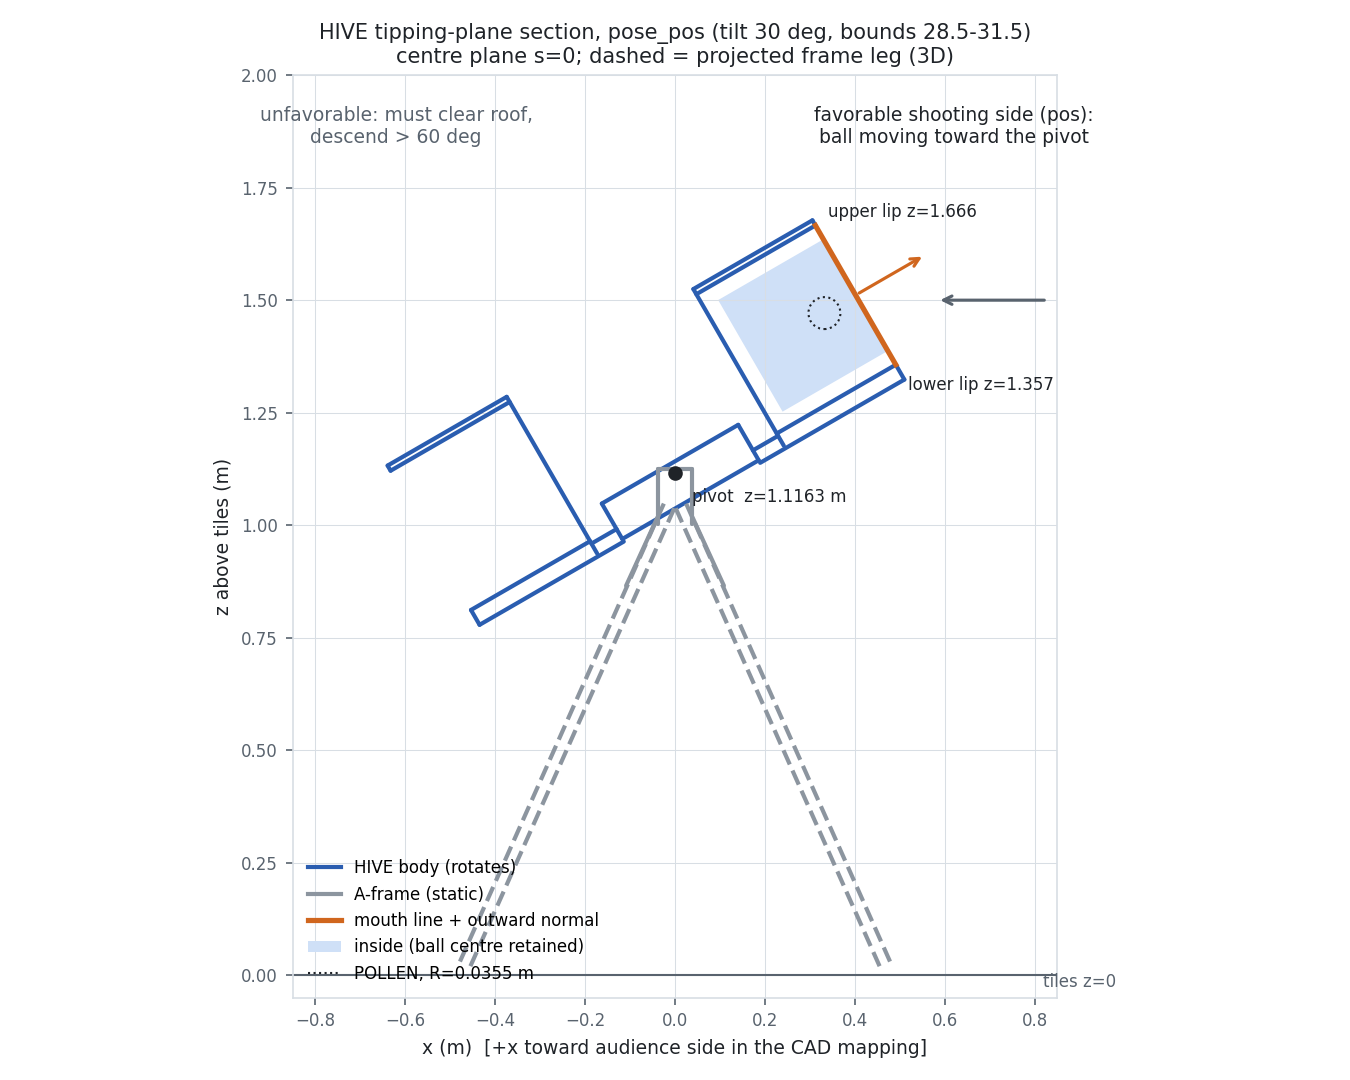
\includegraphics[width=0.78\linewidth]{hive_section_pose_pos.png}
  \caption{HIVE tipping-plane section in \code{pose\_pos} at the $30^\circ$\confirmed{} tilt
    (bounds $28.80$--$31.77^\circ$\derived), centre plane $s=0$. Blue: HIVE body (rotates about the
    pivot at $z_p=1.1163$\,\unit{m}\confirmed); grey: static A-frame (dashed legs are projected from
    3D); orange: mouth line and its outward normal $\vect{n}$; shaded: inside region $\mathcal{I}$
    for the ball centre; dotted circle: POLLEN with $R=0.0355$\,\unit{m}\confirmed. The geometry is
    derived from the official CAD (Section~\ref{sec:geometry}); it is not a model prediction. In
    this pose the favourable side is on the right; an unfavourable-side shot comes from the left and
    must clear the roof.}
  \label{fig:hive-section}
\end{figure}

\section{Problem setup, HIVE geometry and the clean-entry criterion}
\label{sec:geometry}

% Sources: src/hive.py, data/hive_geometry.json, docs/01_hive_geometry.md,
% src/feasibility.py (Geometry.make, evaluate_gate, grid_from_candidates).
% Every worked number in this section was recomputed by running python against the
% repository code on 2026-10-30 (hive.Hive.from_json, Hive.classify_path,
% hive.classify_detail, feasibility.integrate_batch, feasibility.evaluate_gate).

Before any physics of spin can be judged, we need a precise answer to a purely geometric
question: \emph{what does a ball path have to look like to count as ``in''?} This section sets up
the coordinate frames, describes the HIVE cross-section that the model uses, defines the
\emph{clean-entry} test exactly as the code applies it, and derives from the geometry alone how
steeply the ball must be falling when it arrives from the unfavourable side. Everything later in
the paper (drag, Magnus lift, the launcher) only changes \emph{which paths} the robot can make;
this section decides \emph{which paths score}.

\subsection{The question in two dimensions}
\label{sec:geometry-question}

The target is the upward-facing CELL of the pivoting HIVE at the centre of the field. The HIVE is
one rigid beam with a box-shaped CELL at each end. It rests on a damper stop, so one CELL points up
and outward and the other points down and outward. A shot from the side the up CELL faces is
the \emph{favourable} side. A shot from the other side is the \emph{unfavourable} side: the up CELL's
roof is between the robot and the mouth. Our question is whether backspin from a single powered
wheel can bend a POLLEN path enough to score from the unfavourable side.

The model works in the vertical \emph{tipping plane}, the plane in which the CELLS rotate. It
uses the cross-section of the HIVE at its centre plane. A pure backspin shot fired in that plane
stays in it, so a two-dimensional (2D) model is enough for centred shots. Off-centre shots and the
CELL side walls are three-dimensional effects that this section treats only as a stated
limitation (Section~\ref{sec:geometry-assumptions}).

\subsection{Frames}
\label{sec:geometry-frames}

\paragraph{HIVE frame.} The origin is on the tile surface directly below the HIVE pivot axis, at
the HIVE centre plane. The axis $x$ (in \unit{m}) is horizontal and lies in the tipping plane, with
$+x$ pointing toward the audience side of the field. The axis $z$ (in \unit{m}) points up, and $y$
(in \unit{m}) runs along the pivot axis. The pivot axis is at height
\begin{equation}
  z_p = 1.11633\ \text{\unit{m}}\text{\confirmed},
  \label{eq:geometry-pivot}
\end{equation}
which is $43.95$\,\unit{in}\confirmed{} above the tiles (Competition Manual 9.6.1 and the official
field CAD). A point in the tipping plane is written $\vect{p} = (x, z)$.

\paragraph{Cell-local frame.} The HIVE body is stored once, in a frame that rotates with it. The
coordinate $u$ (in \unit{m}) runs along the cell axis, from the pivot outward toward the mouth of
the CELL that is up; $u > 0$ is the up CELL and $u < 0$ the down CELL. The coordinate $w$ (in
\unit{m}) is perpendicular to $u$ and points toward the CELL roof. Both CELLS have their roofs on
the $+w$ side, so the body is mirror-symmetric about $u = 0$. The lateral coordinate $s$ (in
\unit{m}) runs across the CELL opening; $s = 0$ is the centre plane, the plane used in this paper.

\paragraph{From cell-local to HIVE frame.} Let $\tau$ (in rad, quoted in degrees) be the
\emph{tilt}, the angle of the cell axis above the horizontal. Let $\sigma \in \{+1, -1\}$ be the
pose sign: $\sigma = +1$ when the up CELL is on the $+x$ side and $\sigma = -1$ when it is on the
$-x$ side. The code (\code{Hive.from\_json}, inner function \code{world}) places a cell-local point
$(u, w)$ in the HIVE frame in two steps. First it rotates by $\tau$:
\begin{equation}
  \begin{pmatrix} x' \\ z' - z_p \end{pmatrix}
  =
  \begin{pmatrix} \cos\tau & -\sin\tau \\ \sin\tau & \cos\tau \end{pmatrix}
  \begin{pmatrix} u \\ w \end{pmatrix}.
  \label{eq:geometry-rotation}
\end{equation}
Then it mirrors the horizontal coordinate when the up CELL is on the $-x$ side, $x = \sigma x'$.
Combining the two steps gives
\begin{align}
  x &= \sigma\,(u\cos\tau - w\sin\tau), \label{eq:geometry-world-x}\\
  z &= z_p + u\sin\tau + w\cos\tau. \label{eq:geometry-world-z}
\end{align}
Equations~\eqref{eq:geometry-world-x}--\eqref{eq:geometry-world-z} are used whenever the tilt or the pivot
height differ from their nominal values. At the nominal pose the code reads pre-computed
HIVE-frame segments from \code{data/hive\_geometry.json}; these agree with
\eqref{eq:geometry-world-x}--\eqref{eq:geometry-world-z} to the five decimals stored.

\paragraph{Shot frame.} The flight solver always fires toward $+x$. A shooter standing on the
$x < 0$ side therefore uses the HIVE frame unchanged. A shooter on the $x > 0$ side fires toward
$-x$, so the code mirrors the \emph{geometry} ($x \to -x$, \code{Hive.mirrored}) instead of the
trajectory. In the shot frame the robot releases the ball at
\begin{equation}
  \vect{p}_r = (x_r, z_r) = (-d,\; h),
  \label{eq:geometry-release}
\end{equation}
where $d$ (in \unit{m}) is the horizontal distance from the release point to the pivot plane
$x = 0$, and $h$ (in \unit{m}) is the height of the ball \emph{centre} above the tiles at release.

\subsection{The cross-section and its key points}
\label{sec:geometry-section}

Table~\ref{tab:geometry-local} lists the cell-local coordinates that set the mouth. All of them come from
the official field CAD (STEP file, parsed by the project), at the centre plane $s = 0$.

\begin{table}[h]
  \centering
  \caption{Cell-local coordinates of the up CELL at $s = 0$ (from \code{body\_local} in
  \code{data/hive\_geometry.json}).}
  \label{tab:geometry-local}
  \begin{tabular}{@{}lll@{}}
    \toprule
    Symbol & Meaning & Value \\
    \midrule
    $u_M$ & mouth plane (outer rib face) & $0.54508$\,\unit{m}\confirmed \\
    $u_B$ & back wall (back skin) & $0.23952$\,\unit{m}\confirmed \\
    $w_F$ & floor (top of the bottom skin) & $-0.03734$\,\unit{m}\confirmed \\
    $w_C$ & ceiling (roof underside at the pentagon peak) & $0.32004$\,\unit{m}\confirmed \\
    $w_T$ & roof top (envelope of the rib tops) & $0.33325$\,\unit{m}\confirmed \\
    \bottomrule
  \end{tabular}
\end{table}

\paragraph{Mouth length.} The mouth runs along the line $u = u_M$ from the lower lip
$(u_M, w_F)$ to the upper lip $(u_M, w_C)$. Its length is
\begin{equation}
  L = w_C - w_F = 0.32004 - (-0.03734) = 0.35738\ \text{\unit{m}}\text{\derived}.
  \label{eq:geometry-mouth-length}
\end{equation}
The CELL depth is $u_M - u_B = 0.30556$\,\unit{m}\derived{} (manual: about $12$\,\unit{in}\confirmed).

\paragraph{Worked example: the lips in the HIVE frame.} Take $\sigma = +1$ and
$\tau = 30^\circ$\confirmed, so $\cos\tau = 0.86603$\derived{} and $\sin\tau = 0.5$\derived.
For the lower lip, $(u, w) = (0.54508, -0.03734)$, equations
\eqref{eq:geometry-world-x}--\eqref{eq:geometry-world-z} give
\begin{align*}
  x &= 0.54508 \times 0.86603 - (-0.03734)\times 0.5\\
    &= 0.47205 + 0.01867 = 0.49072\ \text{\unit{m}}\text{\derived},\\
  z &= 1.11633 + 0.54508 \times 0.5 + (-0.03734)\times 0.86603\\
    &= 1.11633 + 0.27254 - 0.03234 = 1.35653\ \text{\unit{m}}\text{\derived}.
\end{align*}
That is $53.41$\,\unit{in}\derived, inside the Field Acceptance Checklist value of
$53.5 \pm 0.5$\,\unit{in}\confirmed. Running the same formula in python for the other key points
gives Table~\ref{tab:geometry-keypoints}.

\begin{table}[h]
  \centering
  \caption{Key points of the up CELL, pose \code{pose\_pos}, $\tau = 30^\circ$ (python, \code{hive.py}).}
  \label{tab:geometry-keypoints}
  \begin{tabular}{@{}lrrl@{}}
    \toprule
    Point & $x$ (\unit{m}) & $z$ (\unit{m}) & Official check \\
    \midrule
    Lower lip $(u_M, w_F)$ & $0.49072$\derived & $1.35653$\derived & $53.5$\,\unit{in}\confirmed{} (checklist) \\
    Upper lip $(u_M, w_C)$ & $0.31203$\derived & $1.66603$\derived & $65.6$\,\unit{in}\confirmed{} (Fig.\ 9-10) \\
    Roof top at mouth $(u_M, w_T)$ & $0.30543$\derived & $1.67747$\derived & highest point of the HIVE \\
    Roof top at back $(u_B, w_T)$ & $0.04081$\derived & $1.52469$\derived & -- \\
    \bottomrule
  \end{tabular}
\end{table}

\paragraph{Obstacles.} The code treats the HIVE as a set of solid line segments in the $(x, z)$
plane. Segment $j$ runs from $\vect{a}_j$ to $\vect{b}_j$ (both in \unit{m}). Each pose has
$16$\derived{} CELL segments (8 per CELL: back wall, roof outer, upper lip, roof inner, floor,
lower lip, underside, tube top), $4$\derived{} pivot-plate segments, and $9$\derived{} static
A-frame segments. Four of the A-frame segments are the legs. They slant across the field, so at
$s = 0$ only their top exists; the file flags them \code{projected}, and the code drops them by
default (\code{include\_projected=False}). The default obstacle set therefore has
$25$\derived{} segments ($29$\derived{} with the legs). The A-frame does not rotate with the HIVE.

\subsection{Poses, the mouth normal and the two sides}
\label{sec:geometry-poses}

\paragraph{Poses.} The HIVE has two resting poses. In \code{pose\_pos} the up CELL is on the
$+x$ (audience) side, $\sigma = +1$. In \code{pose\_neg} it is on the $-x$ side, $\sigma = -1$.
\code{pose\_neg} is the exact mirror image ($x \to -x$) of \code{pose\_pos}. Every TIP flips the pose.

\paragraph{Outward normal of the mouth.} The mouth lies on $u = u_M$, so the direction pointing
out of the CELL through the mouth is the cell-local unit vector $(1, 0)$. Rotating it with
\eqref{eq:geometry-rotation} gives $(\cos\tau, \sin\tau)$, and the mirror multiplies the $x$ part by
$\sigma$:
\begin{equation}
  \vect{n} = (\sigma\cos\tau,\; \sin\tau).
  \label{eq:geometry-normal}
\end{equation}
This is exactly the code's \code{normal = np.array([sp * ct, st])}. At $\tau = 30^\circ$\confirmed{}
and $\sigma = +1$, $\vect{n} = (0.86603, 0.5)$\derived: the mouth faces outward and $30^\circ$\derived{}
above the horizontal. The mouth \emph{line} is perpendicular to $\vect{n}$, and in \code{pose\_pos}
its direction from lower to upper lip is $\vect{m} = (-\sin\tau, \cos\tau) = (-0.5, 0.86603)$\derived.

\paragraph{Which way is ``in''?} A ball with velocity $\vect{v} = (v_x, v_z)$ (in \unit{m/s})
is moving into the CELL through the mouth only if its velocity points against the outward normal:
\begin{equation}
  \vect{v}\cdot\vect{n} < 0.
  \label{eq:geometry-inward}
\end{equation}

\paragraph{Favourable and unfavourable sides.} The \emph{favourable} side is the side the up CELL
is on (\code{favorable\_side}: \code{"pos"} for \code{pose\_pos}, \code{"neg"} for
\code{pose\_neg}). A ball fired from there travels toward the pivot, which is roughly
$-\vect{n}$, so \eqref{eq:geometry-inward} is easy to satisfy. The \emph{unfavourable} side is the
other one: the ball travels away from the shooter in the same direction as $\vect{n}_x$, so it can
only satisfy \eqref{eq:geometry-inward} by falling steeply (Section~\ref{sec:geometry-steep}). In the code
(\code{feasibility.Geometry.make}) the unfavourable case is \code{pose\_pos} used as it is, with the
shooter at $x = -d$ firing toward $+x$; the favourable case is the same HIVE mirrored. Results for
\code{pose\_neg} are the exact mirror image and are not computed separately.

\subsection{Tilt and its bounds}
\label{sec:geometry-tilt}

The nominal tilt is $\tau_0 = 30^\circ$\confirmed: Fig.\ 9-10 of the manual labels it, and the CAD
base tube measures $30.0^\circ$\confirmed. Real fields differ, so we bound it using the one
tilt-sensitive number the field checklist controls, the lower-lip height.

\paragraph{Step 1: lip height as a function of tilt.} From \eqref{eq:geometry-world-z} with
$(u, w) = (u_M, w_F)$:
\begin{equation}
  z_{\mathrm{lip}}(\tau) = z_p + u_M\sin\tau + w_F\cos\tau.
  \label{eq:geometry-zlip}
\end{equation}

\paragraph{Step 2: sensitivity.} Differentiating \eqref{eq:geometry-zlip} with $z_p$ held fixed,
\begin{equation}
  \frac{\mathrm{d}z_{\mathrm{lip}}}{\mathrm{d}\tau} = u_M\cos\tau - w_F\sin\tau .
  \label{eq:geometry-dzdtau}
\end{equation}
Comparing with \eqref{eq:geometry-world-x} shows that this is exactly $x_{\mathrm{lip}}$ for
$\sigma = +1$: the lip moves up at a rate equal to its horizontal distance from the pivot, as
expected for a rotation about the pivot. At $\tau_0$ it is $0.49072$\,\unit{m/rad}\derived{} $=
19.32$\,\unit{in/rad}\derived{} $= 0.3372$\,\unit{in/deg}\derived.

\paragraph{Step 3: invert for the tolerance.} The checklist allows
$\Delta z_{\mathrm{lip}} = \pm 0.5$\,\unit{in}\confirmed. With the pivot at its nominal height,
\begin{equation}
  \Delta\tau \approx \frac{\Delta z_{\mathrm{lip}}}{\mathrm{d}z_{\mathrm{lip}}/\mathrm{d}\tau}
  = \frac{0.5}{0.3372} = 1.48^\circ\text{\derived} \;\to\; \tau \in [28.5^\circ, 31.5^\circ]\text{\derived}.
  \label{eq:geometry-tilt-bound}
\end{equation}
If the pivot height is also off by the manual's general $\pm 1$\,\unit{in}\confirmed{} tolerance,
the lip can move $1.5$\,\unit{in}\derived{} for the same checklist reading, giving
$1.5/0.3372 = 4.45^\circ$\derived, rounded to the wide bounds $[25.5^\circ, 34.5^\circ]$\derived{}
(\code{low\_wide}, \code{high\_wide}). The code re-poses the body at any tilt with
\eqref{eq:geometry-world-x}--\eqref{eq:geometry-world-z}; Table~\ref{tab:geometry-tilt} in
Section~\ref{sec:geometry-steep} shows how the entry requirement moves with $\tau$.

\subsection{Configuration space: inflating the obstacles by the ball radius}
\label{sec:geometry-cspace}

A real ball touches a wall when its \emph{surface} reaches the wall. It is easier to track one
point, the ball centre, and grow every obstacle by the ball radius instead. This is the
\emph{configuration-space} idea, and it is how \code{hive.py} works. The POLLEN radius is
\begin{equation}
  R = 0.0355\ \text{\unit{m}}\text{\confirmed}
  \label{eq:geometry-radius}
\end{equation}
(manual 9.8: diameter ``approximately'' $7.1$\,\unit{cm}\confirmed, so about $\pm 1$\,\unit{mm}\assumed{}
is uncertain).

\paragraph{Distance to one segment.} For a ball centre $\vect{p}$ and segment $j$, the code
(\code{seg\_point\_dist}) first finds the nearest point's position along the segment and clips it to
the segment:
\begin{equation}
  \lambda_j^\ast = \operatorname{clip}\!\left(
  \frac{(\vect{p}-\vect{a}_j)\cdot(\vect{b}_j-\vect{a}_j)}{\lVert\vect{b}_j-\vect{a}_j\rVert^2},\;0,\;1\right),
  \qquad
  \vect{q}_j = \vect{a}_j + \lambda_j^\ast(\vect{b}_j-\vect{a}_j).
  \label{eq:geometry-nearest}
\end{equation}
The clip is what gives the inflated segment its rounded end caps: beyond an end, the nearest
point is the end itself. The distance is $\delta_j(\vect{p}) = \lVert\vect{p} - \vect{q}_j\rVert$ (in \unit{m}).

\paragraph{Clearance.} The clearance (in \unit{m}) is the smallest gap between the ball surface and
any obstacle:
\begin{equation}
  c(\vect{p}) = \min_j \delta_j(\vect{p}) - R .
  \label{eq:geometry-clearance}
\end{equation}
The ball is in \emph{contact} when $c(\vect{p}) < 0$ (strictly; $c = 0$ is a graze and not a contact).

\paragraph{Along a path.} A path is a list of centre positions $\vect{p}_0, \vect{p}_1, \dots$ at
the solver's time steps. The exact classifier (\code{Hive.classify\_path}) tests every \emph{chord}
$\vect{p}_k\vect{p}_{k+1}$ against every obstacle with the exact segment-to-segment distance
(\code{seg\_seg\_dist}), so contact between samples is not missed. The sweep
(\code{evaluate\_gate}) uses a precomputed clearance grid instead (\code{CSpaceRaster}), with cells
of side $\Delta = 1$\,\unit{mm}\assumed. It looks up the cell containing each sample. Because the
distance function changes by at most $1$\,\unit{m} per metre moved, the lookup error is at most
$\Delta/\sqrt{2} = 0.71$\,\unit{mm}\derived.

\subsection{The mouth gate and the inside region}
\label{sec:geometry-gate}

\paragraph{Inside region.} The code calls a ball centre \emph{inside} the CELL when it lies in the
quadrilateral $\mathcal{I}$ whose cell-local corners are
\begin{equation}
  \mathcal{I}:\quad u \in [\,u_B + R,\; u_M\,], \qquad w \in [\,w_F + R,\; w_C - R\,].
  \label{eq:geometry-inside}
\end{equation}
In words: behind the mouth plane, and at least one radius away from the back wall, the floor and the
ceiling. It is mapped to the HIVE frame with \eqref{eq:geometry-world-x}--\eqref{eq:geometry-world-z}. Note
that the edge on the mouth plane is \emph{not} moved in by $R$: the ball counts as inside as soon as
its centre is behind the mouth plane.

\paragraph{Gate.} The \emph{gate} is the edge of $\mathcal{I}$ that lies on the mouth plane
(\code{Hive.gate}), ordered low end first:
\begin{equation}
  \vect{A} = \mathrm{world}(u_M,\; w_F + R), \qquad \vect{B} = \mathrm{world}(u_M,\; w_C - R),
  \label{eq:geometry-gate}
\end{equation}
where $\mathrm{world}(\cdot)$ is \eqref{eq:geometry-world-x}--\eqref{eq:geometry-world-z}. Its length is
\begin{equation}
  L_g = (w_C - R) - (w_F + R) = L - 2R = 0.35738 - 0.071 = 0.28638\ \text{\unit{m}}\text{\derived}.
  \label{eq:geometry-gate-length}
\end{equation}
For \code{pose\_pos} at $\tau = 30^\circ$\confirmed{} the code gives
$\vect{A} = (0.47298, 1.38728)$\,\unit{m}\derived{} and $\vect{B} = (0.32979, 1.63529)$\,\unit{m}\derived.
The gate is the window the ball \emph{centre} must pass through; the ball surface then just clears
the lips.

\subsection{The clean-entry criterion}
\label{sec:geometry-clean}

\paragraph{Definition.} A path is \emph{clean} when the ball centre crosses the gate
$\overline{\vect{A}\vect{B}}$ moving inward, \eqref{eq:geometry-inward}, and the clearance
\eqref{eq:geometry-clearance} stayed non-negative at every earlier point of the path. Contact
\emph{after} the crossing (for example with the floor) does not change the label; whether such a
ball stays in is the job of the contact model. The exact classifier returns one of three labels:
\code{clean}; \code{hit:<name>}, the first obstacle touched before entry; or \code{miss}, when the
path reaches neither (for example it falls short onto the field).

\paragraph{How the sweep finds gate crossings.} Without wind, drag and Magnus forces do not depend
on position. So a launch with speed $v$ (in \unit{m/s}), elevation $\theta$ (in degrees) and spin
gives one path \emph{shape} $\vect{\Pi}(t) = (\Pi_x(t), \Pi_z(t))$ (in \unit{m}, starting at
$(0,0)$ at time $t = 0$\,\unit{s}), and the release point only shifts it:
\begin{equation}
  \vect{p}(t) = \vect{p}_r + \vect{\Pi}(t) = \bigl(-d + \Pi_x(t),\; h + \Pi_z(t)\bigr).
  \label{eq:geometry-translate}
\end{equation}
\code{evaluate\_gate} uses this to avoid re-integrating for every release point. For a fixed $h$,
it keeps every sample $k$ of every path that satisfies two conditions:
\begin{align}
  A_z \le h + \Pi_z(t_k) &\le B_z, \label{eq:geometry-band}\\
  \dot{\vect{\Pi}}(t_k)\cdot\vect{n} &< 0. \label{eq:geometry-band-inward}
\end{align}
The first condition says the sample is at a height where the gate is; the second is
\eqref{eq:geometry-inward}. Because the gate is a straight, non-horizontal segment, a height fixes a
unique point on it. Let $s_g$ be the fraction along the gate (0 at $\vect{A}$, 1 at $\vect{B}$):
\begin{equation}
  s_g = \frac{h + \Pi_z(t_k) - A_z}{B_z - A_z}, \qquad
  x_g = A_x + s_g\,(B_x - A_x).
  \label{eq:geometry-gate-fraction}
\end{equation}
Requiring the shifted sample to sit exactly on that gate point, $-d + \Pi_x(t_k) = x_g$, gives the
one release distance at which this sample enters:
\begin{equation}
  d = \Pi_x(t_k) - x_g .
  \label{eq:geometry-d-from-gate}
\end{equation}
Candidates outside the swept range widened by $0.06$\,\unit{m}\assumed{} at each end,
$d \in [0.49, 1.81]$\,\unit{m}\derived{} (grid $0.55$ to $1.75$\,\unit{m}\assumed), are dropped. Each
remaining candidate is clean if the raster clearance is $\ge 0$ at every sample from the first one
whose shifted $x$ has reached the left edge of the raster box up to and including sample $k$
(samples outside the box count as free). (For a path whose $v_x$ reverses, the check
starts at the first sample.) Two consecutive clean samples $k, k+1$ of the same path bound a
continuous interval of clean release distances, and \code{grid\_from\_candidates} marks every grid
value of $d$ inside it as clean. The exact classifier reaches the same label in a different way:
the first sample inside $\mathcal{I}$ before any chord with negative clearance. The two agree
because the only way into $\mathcal{I}$ from outside without contact is through the gate.

% CODE/CODE: evaluate_gate reports the descent angle as atan2(-vz, vx) (signed vx, so it can
% exceed 90 deg when backspin reverses vx); Hive.classify_path reports atan2(-vz, |vx|).
% They agree whenever vx > 0 at entry.

\paragraph{Worked example: one shot through the gate.} To check the formulas by hand we use a
vacuum path (no air at all), so that $\vect{\Pi}(t)$ is a parabola. Air is added in later
sections. Take $v = 7.0$\,\unit{m/s}\assumed, $\theta = 81.0^\circ$\assumed, $h = 0.737$\,\unit{m}\assumed{}
and $d = 1.00$\,\unit{m}\assumed, with $g = 9.80665$\,\unit{m/s\textsuperscript{2}}\confirmed{}
(standard gravity, \code{flight.G\_STANDARD}). Then
$v_x = v\cos\theta = 1.0950$\,\unit{m/s}\derived{} and $v_{z0} = v\sin\theta = 6.9138$\,\unit{m/s}\derived.

\emph{Step 1: crossings of the mouth line.} The centre is on the mouth line when
$(\vect{p}(t) - \vect{A})\cdot\vect{n} = 0$. With $\vect{p}(t) = (-d + v_x t,\; h + v_{z0}t - \tfrac12 g t^2)$
this is a quadratic in $t$:
\begin{equation}
  \underbrace{\bigl(-\tfrac12 g\,n_z\bigr)}_{c_2} t^2
  + \underbrace{\bigl(n_x v_x + n_z v_{z0}\bigr)}_{c_1} t
  + \underbrace{\bigl(n_x(-d - A_x) + n_z(h - A_z)\bigr)}_{c_0} = 0 .
  \label{eq:geometry-quadratic}
\end{equation}
Its roots are $t_1 = 0.5057$\,\unit{s}\predicted{} and $t_2 = 1.2911$\,\unit{s}\predicted.

\emph{Step 2: test each crossing.} At $t_1$ the ball is still rising
($v_z = +1.954$\,\unit{m/s}\predicted), $\vect{v}\cdot\vect{n} = +1.926$\,\unit{m/s}\predicted{} (outward),
and $s_g = 6.42$\predicted{}, far outside $[0, 1]$: the ball passes the extended mouth line high above
the HIVE. It fails both \eqref{eq:geometry-band} and \eqref{eq:geometry-band-inward}. At $t_2$ the centre is at
$(0.4138, 1.4897)$\,\unit{m}\predicted, $s_g = 0.413$\predicted{} (inside the gate),
$v_z = -5.748$\,\unit{m/s}\predicted{} and $\vect{v}\cdot\vect{n} = -1.926$\,\unit{m/s}\predicted{}
(inward). This is the entry.

\emph{Step 3: no earlier contact.} \code{hive.classify\_detail} on the exact parabola returns
\code{clean} with a minimum clearance of $30.5$\,\unit{mm}\predicted{} before entry, reached as the
ball passes the upper lip. The raster sweep (\code{evaluate\_gate} with \code{grid\_from\_candidates}) gives
$28.3$\,\unit{mm}\predicted{} for the same cell. The difference is not raster error: the grid
cell at $d = 1.00$\,\unit{m}\assumed{} takes the smaller margin of the two bracketing gate samples, which
sit at $d = 1.0025$\,\unit{m}\predicted{} and $0.9981$\,\unit{m}\predicted{} (one solver step of $\Delta t = 2$\,\unit{ms}\assumed{}, so
$v_x\,\Delta t \approx 2.2$\,\unit{mm}\derived{} apart); the exact classifier at
$d = 1.0025$\,\unit{m}\predicted{} gives $28.0$\,\unit{mm}\predicted.
% CHECK: re-run 2026-10-30. Raster margins 28.34 / 32.31 mm at d = 1.0025 / 0.9981 m;
% exact classify_path 27.99 / 32.35 mm. The raster lookup error is <= 0.71 mm either way.

\emph{Step 4: the apex.} The highest point is at $t = v_{z0}/g = 0.705$\,\unit{s}\predicted{},
$z = h + v_{z0}^2/(2g) = 3.174$\,\unit{m}\predicted. There $v_z = 0$ but the ball is still moving
sideways at $v_x = 1.095$\,\unit{m/s}\predicted; it is not stationary.

\emph{Step 5: the neighbours.} Keeping $v = 7.0$\,\unit{m/s}\assumed{} and changing only $\theta$:
$78.0^\circ$\assumed{} is a \code{miss}, $80.5^\circ$\assumed{} is \code{hit:up\_floor}
(clearance on the first touching chord $-1.6$\,\unit{mm}\predicted), $81.5^\circ$\assumed{} is
\code{hit:up\_roof\_outer} ($-3.9$\,\unit{mm}\predicted) and $84.0^\circ$\assumed{} is
\code{hit:pivot\_plate\_top}. The overlap reported at first contact depends on the time step of
the path samples, so only its sign is meaningful.
% CHECK: -1.6 / -3.9 mm from flight.simulate (vacuum, dt_max = 1 ms) + classify_detail; the
% exact parabola sampled at 0.1 ms gives -0.3 / -0.1 mm, at 2 ms -5.5 / -3.9 mm. The earlier
% draft values (-0.4 / -2.3 mm) were not reproducible.
In the sweep (\code{evaluate\_gate} with \code{grid\_from\_candidates}), on a sub-grid
($v$ from $5.0$\,\unit{m/s}\assumed{} to $9.0$\,\unit{m/s}\assumed{} in $0.1$\,\unit{m/s}\assumed{} steps,
$\theta$ from $60^\circ$\assumed{} to $89.75^\circ$\assumed{} in $0.25^\circ$\assumed{} steps) at this
$(h, d)$, $82$\predicted{} launches reach the gate and $47$\predicted{} of them are clean; the other
$35$\predicted{} first touch \code{up\_roof\_outer} ($22$\predicted) or \code{up\_upper\_lip}
($13$\predicted). The clean launches form a thin diagonal band in the $(v, \theta)$ plane. This is a
statement about the model in vacuum, not about how often a real launcher would score.

\subsection{Steepness on the unfavourable side: the minimum descent angle}
\label{sec:geometry-steep}

We now derive, from the geometry alone, how steeply the ball must fall to enter from the
unfavourable side. Work in the unfavourable shot frame: \code{pose\_pos}, $\sigma = +1$, shooter
at $x = -d$, ball moving toward $+x$.

\paragraph{Descent angle.} Define the descent angle $\varphi$ (in degrees) of the velocity, measured
below the horizontal and positive when falling, as the code does:
\begin{equation}
  \varphi = \operatorname{atan2}(-v_z,\; v_x), \qquad \vect{v} = \lVert\vect{v}\rVert\,(\cos\varphi,\; -\sin\varphi).
  \label{eq:geometry-descent}
\end{equation}

\paragraph{Step 1: the kinematic condition.} Insert \eqref{eq:geometry-descent} and
\eqref{eq:geometry-normal} into \eqref{eq:geometry-inward}:
\begin{equation}
  \vect{v}\cdot\vect{n} = \lVert\vect{v}\rVert\,(\cos\varphi\cos\tau - \sin\varphi\sin\tau)
  = \lVert\vect{v}\rVert\cos(\varphi + \tau) < 0 .
  \label{eq:geometry-vdotn}
\end{equation}
For a ball still moving toward $+x$ ($-90^\circ < \varphi < 90^\circ$) this needs
$\varphi + \tau > 90^\circ$, so
\begin{equation}
  \varphi > \varphi_{\mathrm{kin}} = 90^\circ - \tau = 60^\circ\text{\derived}.
  \label{eq:geometry-phi-kin}
\end{equation}
This is the ``steeper than $60^\circ$'' rule. It only says the ball is moving into the plane of the
mouth; it says nothing yet about fitting past the lips. It is convenient to measure the excess
over this angle,
\begin{equation}
  \alpha = \varphi + \tau - 90^\circ ,
  \label{eq:geometry-alpha}
\end{equation}
so that \eqref{eq:geometry-phi-kin} reads $\alpha > 0$.

\paragraph{Step 2: the roof.} The highest point of the HIVE is the roof top at the mouth,
$\vect{T} = (0.30543, 1.67747)$\,\unit{m}\derived{} (Table~\ref{tab:geometry-keypoints}). Every gate point
has $x > 0.3298$\,\unit{m}\derived{} and the release has $x = -d < 0$, so the centre must cross the
vertical line $x = x_T$. At that moment the centre is directly above $\vect{T}$ (below it is inside
the HIVE), so the clearance \eqref{eq:geometry-clearance} is non-negative only if
\begin{equation}
  z(x_T) \ge z_T + R = 1.67747 + 0.0355 = 1.7130\ \text{\unit{m}}\text{\derived}.
  \label{eq:geometry-roof}
\end{equation}
So the path must rise at least $1.7130 - h$ above the release point. In vacuum this needs a vertical
launch speed of at least $\sqrt{2g(1.7130 - h)}$, which is $4.375$\,\unit{m/s}\derived{} at
$h = 0.737$\,\unit{m}\assumed. Drag raises this bound; backspin lift can lower it. Both are treated in
later sections.

\paragraph{Step 3: a straight line near the mouth.} Close to the mouth the path is almost straight.
In the worked example the ball reaches the gate at $5.85$\,\unit{m/s}\predicted{} and
$\varphi = 79.2^\circ$\predicted. Under gravity alone its curvature is
$\kappa = g\cos\varphi/\lVert\vect{v}\rVert^2 = 0.054$\,\unit{m\textsuperscript{-1}}\derived, a radius
of $18.7$\,\unit{m}\derived. Over a $0.2$\,\unit{m}\assumed{} chord near the mouth the path departs
from a straight line by about $0.3$\,\unit{mm}\derived. We therefore treat the last part of the path as
a straight line with descent angle $\varphi$.

\paragraph{Step 4: go to the cell-local frame.} Rotate the direction of motion into the cell-local
frame with the inverse of \eqref{eq:geometry-rotation}. Using $\varphi + \tau = 90^\circ + \alpha$,
\begin{equation}
  \hat{\vect{e}}_{uw}
  = \bigl(\cos(\varphi+\tau),\; -\sin(\varphi+\tau)\bigr)
  = (-\sin\alpha,\; -\cos\alpha).
  \label{eq:geometry-local-dir}
\end{equation}
In the CELL's own frame the ball is falling almost parallel to the mouth plane, from the roof side
toward the floor side, while moving inward at the small rate $\sin\alpha$. Let the centre cross the
mouth plane at $(u_M, w_c)$, with $w_F + R \le w_c \le w_C - R$ (on the gate). Before the crossing
the centre was at
\begin{equation}
  \bigl(u_M + \lambda\sin\alpha,\; w_c + \lambda\cos\alpha\bigr), \qquad \lambda \ge 0 ,
  \label{eq:geometry-backray}
\end{equation}
with $\lambda$ (in \unit{m}) the distance travelled back along the path. It is outside the mouth
($u > u_M$) the whole time.

\paragraph{Step 5: clear the upper lip.} The obstacle nearest this ray is the inner corner of the
upper lip, $\vect{C} = (u_M, w_C)$; the rest of the lip and the roof are further away from it. The
distance from $\vect{C}$ to the line through $(u_M, w_c)$ in direction \eqref{eq:geometry-local-dir} is
the length of the cross product of $\vect{C} - (u_M, w_c) = (0,\; w_C - w_c)$ with the unit
direction:
\begin{equation}
  \delta_C = \bigl|\,0\cdot(-\cos\alpha) - (w_C - w_c)(-\sin\alpha)\,\bigr| = (w_C - w_c)\sin\alpha .
  \label{eq:geometry-dist-upper}
\end{equation}
The nearest point lies at $\lambda = (w_C - w_c)\cos\alpha \ge 0$, so it is \emph{before} the
crossing and counts. The clean test needs $\delta_C \ge R$:
\begin{equation}
  w_c \le w_C - \frac{R}{\sin\alpha}.
  \label{eq:geometry-upper-cond}
\end{equation}

\paragraph{Step 6: the lower lip does not bind before entry.} For the lower-lip corner
$\vect{D} = (u_M, w_F)$ the same calculation gives the nearest point at
$\lambda = (w_F - w_c)\cos\alpha < 0$, which is \emph{after} the crossing. Before the crossing the
closest the ball gets to $\vect{D}$ is at the crossing itself, $w_c - w_F \ge R$, which the gate
already guarantees. A ball crossing near the low end may touch the lower lip or floor just after it
enters, but by the definition in Section~\ref{sec:geometry-clean} it is already in.

\paragraph{Step 7: the minimum descent angle.} A clean straight path exists when
\eqref{eq:geometry-upper-cond} leaves room above the gate's low end, $w_C - R/\sin\alpha \ge w_F + R$, that is
$\sin\alpha \ge R/(w_C - w_F - R) = R/(L - R)$. Hence
\begin{equation}
  \boxed{\;\varphi > \varphi_{\mathrm{gate}} = 90^\circ - \tau + \arcsin\!\frac{R}{L - R}\;}
  \label{eq:geometry-phi-gate}
\end{equation}
With $R/(L-R) = 0.0355/0.32188 = 0.1103$\derived, $\arcsin(0.1103) = 6.33^\circ$\derived{} and
$\varphi_{\mathrm{gate}} = 66.33^\circ$\derived{} at $\tau = 30^\circ$\confirmed.

\paragraph{A stricter version: passing both lips.} If we also ask that the ball touch nothing until it
is completely past the mouth plane, the line must also stay $R$ from $\vect{D}$:
$\delta_D = (w_c - w_F)\sin\alpha \ge R$. Combined with \eqref{eq:geometry-upper-cond} this needs
$L\sin\alpha \ge 2R$:
\begin{equation}
  \varphi > \varphi_{\mathrm{fit}} = 90^\circ - \tau + \arcsin\!\frac{2R}{L}
  = 60^\circ + 11.46^\circ = 71.46^\circ\text{\derived}.
  \label{eq:geometry-phi-fit}
\end{equation}
The quantity $L\sin\alpha$ is the width of the mouth as seen along the path. This is the
``about $71.5^\circ$'' figure in the project documents. The code's clean test is
\eqref{eq:geometry-phi-gate}, not \eqref{eq:geometry-phi-fit}.
% CODE/DOC: docs/01_hive_geometry.md section 4 and the "reason" fields of
% data/hive_geometry.json give > ~71.5 deg (60 + asin(2R/0.3574)) as the minimum descent and
% a vertical-drop window of 0.108 m (|x| 0.347-0.455 m). That is the both-lips criterion
% (eq:geometry-phi-fit). The code's clean test (centre crosses the gate before any contact)
% admits straight paths from 66.33 deg and a vertical-drop window of 0.125 m (x 0.348-0.473 m).
% docs/03_clean_entry.md section 2.1 attributes clean gate descents below 71.5 deg (down to
% 68.3 deg) to path curvature; the curvature offset over the mouth is < 1 mm, so the gate
% definition, not curvature, explains the difference. This paper follows the code.

\paragraph{Window width.} The set of clean straight paths at a given $\alpha$ is
$w_c \in [\,w_F + R,\; w_C - R/\sin\alpha\,]$. Measured perpendicular to the path, its width (in \unit{m}) is
\begin{equation}
  W_\perp(\alpha) = \Bigl(w_C - \frac{R}{\sin\alpha} - w_F - R\Bigr)\sin\alpha = (L - R)\sin\alpha - R .
  \label{eq:geometry-window}
\end{equation}
For a vertical drop, $\varphi = 90^\circ$, so $\alpha = \tau$ and the window is horizontal:
$W_\perp = 0.32188 \times 0.5 - 0.0355 = 0.1254$\,\unit{m}\derived. Under the stricter both-lips
rule the same drop leaves $L\sin\tau - 2R = 0.1077$\,\unit{m}\derived. At $\varphi = 70^\circ$\assumed{}
($\alpha = 10^\circ$) the clean window is only $W_\perp = 0.0204$\,\unit{m}\derived, about $0.29$\derived{}
ball diameters ($0.57$\derived{} radii).

\paragraph{Worked check against the code.} We fired families of straight lines at the gate with
\code{Hive.classify\_path} (\code{pose\_pos}, HIVE frame, $400$\assumed{} entry points along the gate per angle)
and bisected on $\varphi$ for the smallest angle with any clean line. Table~\ref{tab:geometry-tilt} compares
the result with \eqref{eq:geometry-phi-gate}. The perpendicular widths found at $\varphi = 70^\circ$,
$72^\circ$ and $90^\circ$ were $0.0202$\predicted, $0.0312$\predicted{} and $0.1249$\,\unit{m}\predicted,
against $0.0204$\derived, $0.0314$\derived{} and $0.1254$\,\unit{m}\derived{} from
\eqref{eq:geometry-window}; the small shortfall comes from the discrete entry points, spaced
$0.72$\,\unit{mm}\derived{} along the gate, so up to one spacing is lost at each end of the window.
% CHECK: re-run 2026-10-30, (n_clean - 1) x spacing x |sin(gate, path)|; draft had
% 0.0201 / 0.0310 / 0.1245 m and a "0.5 mm sampling" that does not match 400 points on 0.286 m.
The vertical drop is clean for $x \in [0.348, 0.4726]$\,\unit{m}\predicted, from one radius right of
the upper lip ($0.31203 + 0.0355 = 0.3475$\,\unit{m}\derived) to the gate's low end
($A_x = 0.47298$\,\unit{m}\derived).

\begin{table}[h]
  \centering
  \caption{Descent-angle limits on the unfavourable side versus tilt. $\varphi_{\mathrm{kin}}$:
  \eqref{eq:geometry-phi-kin}; $\varphi_{\mathrm{gate}}$: \eqref{eq:geometry-phi-gate} (the code's criterion);
  $\varphi_{\mathrm{fit}}$: \eqref{eq:geometry-phi-fit}; ``code'' is the bisection with
  \code{Hive.classify\_path}; $z_{\mathrm{lip}}$ from the re-posed \code{Hive}.}
  \label{tab:geometry-tilt}
  \begin{tabular}{@{}rrrrrr@{}}
    \toprule
    $\tau$ & $z_{\mathrm{lip}}$ (\unit{m}) & $\varphi_{\mathrm{kin}}$ & $\varphi_{\mathrm{gate}}$ & code & $\varphi_{\mathrm{fit}}$ \\
    \midrule
    $25.5^\circ$\derived & $1.3173$\derived & $64.5^\circ$\derived & $70.83^\circ$\derived & -- & $75.96^\circ$\derived \\
    $28.5^\circ$\derived & $1.3436$\derived & $61.5^\circ$\derived & $67.83^\circ$\derived & $67.85^\circ$\predicted & $72.96^\circ$\derived \\
    $30.0^\circ$\confirmed & $1.3565$\derived & $60.0^\circ$\derived & $66.33^\circ$\derived & $66.35^\circ$\predicted & $71.46^\circ$\derived \\
    $31.5^\circ$\derived & $1.3693$\derived & $58.5^\circ$\derived & $64.83^\circ$\derived & $64.85^\circ$\predicted & $69.96^\circ$\derived \\
    $34.5^\circ$\derived & $1.3943$\derived & $55.5^\circ$\derived & $61.83^\circ$\derived & -- & $66.96^\circ$\derived \\
    \bottomrule
  \end{tabular}
\end{table}

A steeper HIVE (larger $\tau$) turns the mouth more toward the sky and lowers every limit one degree
per degree of tilt. The $\arcsin$ term does not depend on tilt because the CELL itself does not change
shape. The worked shot of Section~\ref{sec:geometry-clean} entered at $\varphi = 79.21^\circ$\predicted,
above all three limits at $\tau = 30^\circ$\confirmed.

\subsection{Release point and the robot height limit}
\label{sec:geometry-release}

The release point \eqref{eq:geometry-release} has two free numbers. The distance $d$ is measured from the
release point to the pivot plane $x = 0$ (not to the mouth). The field's inner perimeter wall is at
$|x| = 1.8009$\,\unit{m}\confirmed, so $d$ cannot exceed that. The sweep grid uses
$d$ from $0.55$\,\unit{m}\assumed{} to $1.75$\,\unit{m}\assumed{} in $0.05$\,\unit{m}\assumed{} steps.

The height $h$ is limited by the robot size rule. Manual rule R105 caps the expanded robot at
$H_{\max} = 29$\,\unit{in}\confirmed{} $= 0.7366$\,\unit{m}\confirmed{} measured from the field
surface. The project assumes that the ball centre at release is no higher than this:
\begin{equation}
  h \le H_{\max} = 0.7366\ \text{\unit{m}}\text{\assumed},
  \label{eq:geometry-hmax}
\end{equation}
and the sweep uses $h \in \{0.20, 0.35, 0.50, 0.65, 0.737\}$\,\unit{m}\assumed.
% CODE/DOC: data/hive_geometry.json robot_limits.release_height_note says "ball centre at release
% <= 0.737 m (ball inside the sizing volume)". If the whole ball had to be inside the volume the
% centre limit would be 0.7366 - R = 0.701 m. The code (SweepGrid.h) uses h = 0.737 m as the
% centre height, so this paper follows the code and flags the G416 risk.
% CHECK: the grid value 0.737 m (feasibility.SweepGrid.h) is H_max = 0.7366 m rounded up by
% 0.4 mm, so the top grid row sits 0.4 mm above eq:geometry-hmax; negligible but noted.
If instead the whole ball had to stay inside the sizing volume, the centre limit would be
$H_{\max} - R = 0.701$\,\unit{m}\derived; the code uses the former. The lowest point of the HIVE (the
down CELL's lower lip) is at $0.778$\,\unit{m}\derived{}, above the release, so every shot must rise to
pass over the roof, condition \eqref{eq:geometry-roof}.

\subsection{Assumptions}
\label{sec:geometry-assumptions}

\begin{itemize}
  \item The model is 2D, in the HIVE centre plane $s = 0$, where the mouth is tallest. Off-centre the
        pentagonal roof is lower. For a lateral offset $|s|$, \code{hive.py} lowers the roof segments
        and the top of the mouth by
        \begin{equation}
          \Delta w(s) = (h_0 - h_w)\,\frac{\min(|s|,\, s_{\mathrm{half}})}{s_{\mathrm{half}}},
          \label{eq:geometry-roof-drop}
        \end{equation}
        with peak height $h_0 = 0.3556$\,\unit{m}\confirmed, side-wall height
        $h_w = 0.19329$\,\unit{m}\confirmed{} and half-width $s_{\mathrm{half}} = 0.254$\,\unit{m}\confirmed.
        This is a 2D proxy; the side walls themselves are not modelled.
  \item The obstacles are solid line segments with no thickness of their own. The roof top and the
        underside are envelopes of the ribs, accurate to about $11$\,\unit{mm}\derived. The ballast screw near
        each CELL opening and the three preloaded NECTAR are not modelled.
  \item The four A-frame legs are left out by default, because at $s = 0$ only their tops exist.
  \item The ball is a rigid sphere of radius $R$; its centre is the tracked point.
  \item ``Clean'' means the centre crosses the gate inward with no earlier contact (an assumed
        criterion). Contact after the crossing, and whether the ball then stays in, belongs to the contact
        model. A planned bank shot off the roof is outside this channel (and is a G417 risk).
  \item The tilt is a fixed $30^\circ$\confirmed{} rest angle, with $\pm 1.5^\circ$\derived{} and
        $\pm 4.5^\circ$\derived{} bounds; the HIVE does not move during the shot.
  \item The descent-angle limits \eqref{eq:geometry-phi-gate} and \eqref{eq:geometry-phi-fit} treat the last few
        centimetres of the path as straight.
  \item The release height limit \eqref{eq:geometry-hmax} applies to the ball centre.
  \item The worked shot is in vacuum and illustrates the method only; its numbers are not a prediction
        for POLLEN in air.
\end{itemize}

\section{Flight dynamics: drag, Magnus lift and spin decay}
\label{sec:flight}

% Source of truth: src/flight.py (simulate, _aero, backspin_omega, cl_linear_capped, load_params),
% plus the fixed-step RK4 copies of the same force model in src/feasibility.py (integrate_batch),
% src/robustness.py (integrate3d) and src/contact.py (_acc, _rk4, free_flight).
% Parameter values: research/params_lit.json (the default for new runs; see research/LITERATURE_SYNTHESIS.md).
% Every worked number below was computed on 2026-10-30 by running the repo code with the system python
% after fl.set_aero_path(fl.LIT_PARAMS_PATH).

Once POLLEN leaves the shooter, nothing on the robot can change its path any more.
Three things act on the ball in the air: gravity, air drag and the Magnus force from spin.
This section derives, step by step, exactly what the flight solver \code{src/flight.py} computes.
The goal is to answer two practical questions.
How large is the spin force compared with gravity and drag?
And does adding more backspin keep helping?
In this model the answer to the second question is no: above a certain spin the lift coefficient
stops growing, and extra spin changes nothing.

Every aerodynamic coefficient in this section is taken from an assumed, literature-based range, not
from a POLLEN measurement.
The ranges come from \code{research/params\_lit.json}.
They are based on pickleball and smooth-sphere data, but they are not proven bounds: no one has yet
measured drag, lift or spin decay on a real POLLEN ball.

% ---------------------------------------------------------------------------------------------
\subsection{Frame, state and parameters}
\label{sec:flight-frame}

\paragraph{Motivation.}
Before writing any force we need a coordinate frame and a list of what the solver tracks.
Sign errors in the Magnus force are the most common bug in spin models, so the frame must be fixed first.

\paragraph{Frame.}
The world frame is right-handed.
The axis $x$ is horizontal and points toward the target, $y$ is horizontal and sideways, and $z$ points up.
The unit vectors are $\hat{\vect{x}}$, $\hat{\vect{y}}$ and $\hat{\vect{z}}$.
All quantities are in SI units (m, s, kg, rad).

\paragraph{State.}
The solver integrates a nine-component state: the position of the ball centre $\vect{r}$ (\unit{m}),
its velocity $\vect{v}$ (\unit{m/s}) and its spin (angular velocity) vector $\vect{\omega}$ (\unit{rad/s}).
The ball is treated as a rigid sphere of mass $m$ (\unit{kg}) and outer radius $R$ (\unit{m}).

\paragraph{Parameters.}
Table~\ref{tab:flight-params} lists the physical constants read by \code{load\_params}.
The acceleration of gravity is $g$ (\unit{m/s\textsuperscript{2}}), the air density is $\rho$ (\unit{kg/m\textsuperscript{3}}) and the
kinematic viscosity of air is $\nu$ (\unit{m\textsuperscript{2}/s}).
The frontal (cross-sectional) area of the ball is
\begin{equation}
  A = \pi R^2 ,
  \label{eq:flight-area}
\end{equation}
in \unit{m\textsuperscript{2}}.
With the nominal radius, $A = 3.959\times10^{-3}$\,\unit{m\textsuperscript{2}}\derived.

\begin{table}[htbp]
  \centering
  \caption{Physical constants used by the flight solver (\code{research/params\_lit.json}).
    Only the nominal values of $\rho$, $\nu$, $m$ and $R$ are read by \code{load\_params}; the bounds
    are used by the robustness sweeps.}
  \label{tab:flight-params}
  \small
  \begin{tabular}{@{}lllll@{}}
    \toprule
    Symbol & Meaning & Unit & Nominal & Bounds \\
    \midrule
    $g$    & standard gravity & \unit{m/s\textsuperscript{2}} & 9.80665\confirmed & -- \\
    $\rho$ & air density & \unit{kg/m\textsuperscript{3}} & 1.2\assumed & 1.0\assumed\ to 1.25\assumed \\
    $\nu$  & kinematic viscosity & \unit{m\textsuperscript{2}/s} & $1.5\times10^{-5}$\assumed & $1.45\times10^{-5}$\assumed\ to $1.6\times10^{-5}$\assumed \\
    $m$    & ball mass & \unit{kg} & 0.02495\assumed & 0.0235\assumed\ to 0.0275\assumed \\
    $R$    & outer radius & \unit{m} & 0.0355\confirmed & 0.035\assumed\ to 0.036\assumed \\
    \bottomrule
  \end{tabular}
\end{table}

% Provenance note: m = 24.95 g is the AndyMark listing (0.055 lb), grade C vendor data in params_lit.json,
% not the official CAD or game manual, so it is tagged \assumed (as in the contact section). The radius
% 0.0355 m is the manual's "approximately 2.8 in (7.1 cm)", hence \confirmed.
% Code note: src/flight.py sets AERO_PARAMS_PATH to data/aero_params.json unless the environment variable
% PM001_AERO_PATH is set. Only the command-line entry points of feasibility.py, robustness.py and contact.py
% call set_aero_path(LIT_PARAMS_PATH). A bare fl.load_params() or fl.default_params() (and the unit tests
% test_hive / test_contact) therefore still read the older first-pass file, although DECISIONS.md makes
% params_lit.json the default for new runs. All numbers in this section use params_lit.json explicitly.

\paragraph{Assumptions.}
\begin{itemize}
  \item The world frame is inertial (no Coriolis or centrifugal terms) and the floor is flat.
  \item The ball is a rigid sphere of fixed $m$ and $R$; it does not deform in flight.
  \item $\rho$, $\nu$ and $g$ are constant during a shot.
\end{itemize}

% ---------------------------------------------------------------------------------------------
\subsection{Equations of motion}
\label{sec:flight-eom}

\paragraph{Motivation.}
Newton's second law gives the translation; a simple decay law gives the spin.
The only subtlety is wind: aerodynamic forces depend on how the ball moves \emph{through the air},
not over the floor.

\paragraph{Air-relative velocity.}
Let $\vect{u}$ (\unit{m/s}) be the wind velocity.
The air-relative velocity is
\begin{equation}
  \vect{v}_{\mathrm{rel}} = \vect{v} - \vect{u} .
  \label{eq:flight-vrel}
\end{equation}
Both aerodynamic forces below use $\vect{v}_{\mathrm{rel}}$; gravity does not.
The code accepts a constant $\vect{u}$ or a function $\vect{u}(t,\vect{r})$.
The default is still air, $\vect{u}=\vect{0}$, so then $\vect{v}_{\mathrm{rel}}=\vect{v}$.

\paragraph{Newton's law and the spin law.}
Gravity is $m\vect{g}$ with $\vect{g} = -g\,\hat{\vect{z}}$.
Adding the drag force $\vect{F}_D$ and the Magnus force $\vect{F}_M$ (both in \unit{N}) gives
\begin{align}
  \frac{d\vect{r}}{dt} &= \vect{v}, \label{eq:flight-eom-r}\\
  m\,\frac{d\vect{v}}{dt} &= -m g\,\hat{\vect{z}} + \vect{F}_D(\vect{v}_{\mathrm{rel}}) + \vect{F}_M(\vect{v}_{\mathrm{rel}},\vect{\omega}), \label{eq:flight-eom-v}\\
  \frac{d\vect{\omega}}{dt} &= -k\,\vect{\omega}. \label{eq:flight-eom-w}
\end{align}
Here $k$ (\unit{1/s}) is the spin-decay rate (Section~\ref{sec:flight-decay}).
In \code{\_make\_rhs} the right-hand side is exactly this:
the acceleration is $(\vect{F}_D+\vect{F}_M)/m$ with $g$ subtracted from the $z$ component,
and each spin component is multiplied by $-k$.
No other torque acts on the ball, so the spin axis never turns.

\paragraph{Assumptions.}
\begin{itemize}
  \item The ball is a point mass for translation; only its spin vector is tracked for rotation.
  \item Buoyancy and the added mass of the surrounding air are neglected.
    The air displaced by the outer envelope has a mass of $2.25\times10^{-4}$\,\unit{kg}\derived,
    which is $0.9$\,\%\derived\ of $m$.
  \item The wind is prescribed; the ball's own wake and the robot's airflow are ignored.
\end{itemize}

% ---------------------------------------------------------------------------------------------
\subsection{Drag}
\label{sec:flight-drag}

\paragraph{Motivation.}
Drag is the largest aerodynamic force on POLLEN for almost every parameter set in this model
(the one exception, high lift with low drag, is in Section~\ref{sec:flight-scale}).
It slows the ball and shortens the shot.

\paragraph{Derivation.}
The dynamic pressure $q$ (\unit{Pa}) is the kinetic energy of the oncoming air per unit volume.
The drag magnitude is the dynamic pressure times the frontal area times a dimensionless drag coefficient
$C_d$.
Drag points straight against the air-relative velocity, so we multiply by the unit vector
$-\vect{v}_{\mathrm{rel}}/|\vect{v}_{\mathrm{rel}}|$:
\begin{align}
  q &= \tfrac12\,\rho\,|\vect{v}_{\mathrm{rel}}|^2, \label{eq:flight-q}\\
  |\vect{F}_D| &= q\,C_d\,A, \label{eq:flight-FDmag}\\
  \vect{F}_D &= -|\vect{F}_D|\,\frac{\vect{v}_{\mathrm{rel}}}{|\vect{v}_{\mathrm{rel}}|}
             = -\tfrac12\,\rho\,C_d\,A\,|\vect{v}_{\mathrm{rel}}|\,\vect{v}_{\mathrm{rel}}. \label{eq:flight-drag}
\end{align}
In the last step one factor of $|\vect{v}_{\mathrm{rel}}|$ cancels.
The form $|\vect{v}_{\mathrm{rel}}|\,\vect{v}_{\mathrm{rel}}$ is what \code{\_aero} computes
(\code{kd = -q*cd*vmag}, then \code{kd*vx}, \dots; note that the code's variable \code{q} is
$\tfrac12\rho A$, not the dynamic pressure $q$ of Eq.~\eqref{eq:flight-q}).
It has no division, so drag goes smoothly to zero as $|\vect{v}_{\mathrm{rel}}|\to 0$.

\paragraph{Values.}
$C_d$ is constant during a run.
The bounds are $C_d = 0.33$\assumed\ (low), $0.5$\assumed\ (nominal) and $0.9$\assumed\ (high).
The low end comes from outdoor pickleball free flight; the high end covers a spinning perforated ball,
because smooth-sphere data show that spin raises drag.
The solver also accepts a function $C_d(\mathrm{Re})$ or $C_d(\mathrm{Re},S)$, but no sweep uses one.
% Code vs params_lit: params_lit.json lists an optional spin term Cd = Cd0 + dCd*min(S/0.6, 1). load_params
% returns only the constant low/nominal/high value, so that term is not active in any run.

\paragraph{Worked example.}
Take a launch at $|\vect{v}| = 7$\,\unit{m/s}\assumed\ and elevation $60^\circ$\assumed\ in still air,
so $\vect{v} = (3.5\assumed, 0, 6.062\derived)$\,\unit{m/s}.
With the nominal values, $\tfrac12\rho A = 2.3755\times10^{-3}$\,\unit{kg/m}\derived, so
$|\vect{F}_D| = 2.3755\times10^{-3}\derived \times 0.5\assumed \times 49\derived = 0.0582$\,\unit{N}\derived.
\code{aero\_forces} returns $\vect{F}_D = (-0.02910, 0, -0.05040)$\,\unit{N}\predicted, which is the
same magnitude pointing exactly against $\vect{v}$.
The weight is $mg = 0.2447$\,\unit{N}\derived, so drag is $0.238$\derived\ of the weight at this speed.

\paragraph{Assumptions.}
\begin{itemize}
  \item $C_d$ is constant along the path; no Reynolds-number or spin dependence is active.
  \item No ``knuckle'' side force from the holes is modelled. \code{params\_lit.json} lists a
    non-Magnus hole force as a scatter source, but the solver does not include it.
\end{itemize}

% ---------------------------------------------------------------------------------------------
\subsection{Reynolds number and spin parameter}
\label{sec:flight-Re-S}

\paragraph{Motivation.}
Two dimensionless numbers describe the flow around a spinning ball.
The Reynolds number says which flow regime we are in; the spin parameter says how fast the surface
moves compared with the air.

\paragraph{Reynolds number.}
With the ball diameter $D = 2R$ (\unit{m}),
\begin{equation}
  \mathrm{Re} = \frac{|\vect{v}_{\mathrm{rel}}|\,2R}{\nu}.
  \label{eq:flight-Re}
\end{equation}
For speeds of $2$\assumed, $5$\assumed, $7$\assumed\ and $10$\,\unit{m/s}\assumed\ this gives
$\mathrm{Re} = 9.47\times10^{3}$\derived, $2.37\times10^{4}$\derived, $3.31\times10^{4}$\derived\
and $4.73\times10^{4}$\derived.
This is below the smooth-sphere drag crisis, but it overlaps the band where smooth-sphere lift
data show a dip (the ``lift crisis'' recorded in \code{params\_lit.json}).
In the default model $\mathrm{Re}$ is only a diagnostic: $C_d$ is constant and $C_L$ depends on $S$ alone.
It is reported so that a run can be checked against the range of the literature data.

\paragraph{Spin parameter.}
A point on the equator of the ball moves at speed $|\vect{\omega}|R$ relative to the centre.
The spin parameter is the ratio of that surface speed to the airspeed:
\begin{equation}
  S = \frac{|\vect{\omega}|\,R}{|\vect{v}_{\mathrm{rel}}|}.
  \label{eq:flight-S}
\end{equation}
$S$ has no units.
$S = 1$ means the surface speed equals the airspeed, which is what an ideal no-slip hood gives at the exit.
Note that the code uses the full spin magnitude $|\vect{\omega}|$, not only the part of $\vect{\omega}$
perpendicular to $\vect{v}_{\mathrm{rel}}$.

\paragraph{Regularisation.}
Equation~\eqref{eq:flight-S} divides by zero when the ball is at rest relative to the air.
The code therefore uses
\begin{equation}
  S = \frac{|\vect{\omega}|\,R}{\sqrt{|\vect{v}_{\mathrm{rel}}|^2 + \varepsilon_v^2}},
  \label{eq:flight-S-reg}
\end{equation}
with the regularisation speed $\varepsilon_v = 10^{-6}$\,\unit{m/s}\assumed.
For any airspeed above about $10^{-3}$\,\unit{m/s}\assumed\ the difference is far below measurement accuracy.
% HANDOFF 4A writes S = |omega| R / max(|v_rel|, eps). The code uses sqrt(|v_rel|^2 + eps^2), as here.

\paragraph{Worked example.}
For the launch above, an exit spin parameter $S_0 = 1.06$\assumed\ (the nominal hood value in
\code{params\_lit.json}) needs
$|\vect{\omega}_0| = S_0|\vect{v}|/R = 1.06\assumed\times 7\assumed/0.0355\confirmed = 209.0$\,\unit{rad/s}\derived,
which is $1996$\,\unit{rpm}\derived.
The Reynolds number is $3.31\times10^{4}$\derived.

% ---------------------------------------------------------------------------------------------
\subsection{The Magnus force}
\label{sec:flight-magnus}

\paragraph{Motivation.}
A spinning ball drags the air near its surface around with it.
The flow is deflected to one side, and the ball is pushed to the other side.
This sideways push is the Magnus force.
It is the only way spin changes the flight path in this model.

\paragraph{Magnitude and direction.}
The Magnus force has the same dynamic-pressure form as drag, with a lift coefficient $C_L$ (no units)
in place of $C_d$.
Its direction is perpendicular to both the spin axis and the airflow, given by the cross product
$\vect{\omega}\times\vect{v}_{\mathrm{rel}}$:
\begin{align}
  |\vect{F}_M| &= \tfrac12\,\rho\,C_L\,A\,|\vect{v}_{\mathrm{rel}}|^2, \label{eq:flight-FMmag}\\
  \hat{\vect{n}}_M &= \frac{\vect{\omega}\times\vect{v}_{\mathrm{rel}}}{|\vect{\omega}\times\vect{v}_{\mathrm{rel}}|}, \label{eq:flight-nM}\\
  \vect{F}_M &= |\vect{F}_M|\,\hat{\vect{n}}_M
             = \tfrac12\,\rho\,C_L(S)\,A\,|\vect{v}_{\mathrm{rel}}|^2\,
               \frac{\vect{\omega}\times\vect{v}_{\mathrm{rel}}}{|\vect{\omega}\times\vect{v}_{\mathrm{rel}}|}. \label{eq:flight-FM}
\end{align}
The unit vector $\hat{\vect{n}}_M$ carries only the direction, so the spin rate enters the force
only through $C_L(S)$.
This fact matters a great deal in Section~\ref{sec:flight-lift}.

\paragraph{Regularised form used in the code.}
To keep the direction finite when $\vect{\omega}\times\vect{v}_{\mathrm{rel}}\to\vect{0}$, \code{\_aero}
computes
\begin{equation}
  \vect{F}_M = \tfrac12\,\rho\,C_L(S)\,A\,|\vect{v}_{\mathrm{rel}}|^2\,
  \frac{\vect{\omega}\times\vect{v}_{\mathrm{rel}}}
       {\sqrt{|\vect{\omega}\times\vect{v}_{\mathrm{rel}}|^2 + \varepsilon_v^2|\vect{\omega}|^2}} ,
  \label{eq:flight-FM-reg}
\end{equation}
and sets $\vect{F}_M = \vect{0}$ when $\vect{\omega}=\vect{0}$, when $\vect{v}_{\mathrm{rel}}=\vect{0}$
or when no lift law is given.
Because of the factor $|\vect{v}_{\mathrm{rel}}|^2$ and the bounded $C_L$, the force vanishes smoothly
at zero airspeed; there is no fictitious force from the $1/|\vect{v}_{\mathrm{rel}}|$ in $S$.

\paragraph{Magnus does no work in still air.}
A useful property follows from the cross product.
For any vectors, $(\vect{\omega}\times\vect{v}_{\mathrm{rel}})\cdot\vect{v}_{\mathrm{rel}} = 0$, so
\begin{equation}
  \vect{F}_M\cdot\vect{v}_{\mathrm{rel}} = 0 .
  \label{eq:flight-FM-perp}
\end{equation}
In still air $\vect{v}_{\mathrm{rel}}=\vect{v}$, so the power $\vect{F}_M\cdot\vect{v}$ is zero.
The Magnus force bends the path but cannot speed the ball up or slow it down.
Only gravity and drag change the speed.

\paragraph{Worked example.}
For the launch above ($S_0 = 1.06$\assumed, nominal set, so $C_L = 0.25$\derived; see below),
\code{aero\_forces} returns $\vect{F}_M = (-0.02520, 0, 0.01455)$\,\unit{N}\predicted\ with
$|\vect{F}_M| = 0.0291$\,\unit{N}\predicted.
Check: $2.3755\times10^{-3}\derived\times0.25\derived\times49\derived = 0.0291$\,\unit{N}\derived.
The dot product with $\vect{v} = (3.5, 0, 6.062)$ is
$-0.02520\times3.5 + 0.01455\times6.062 = 0.0000$\derived\ (to four decimals), as
Eq.~\eqref{eq:flight-FM-perp} requires.

\paragraph{Assumptions.}
\begin{itemize}
  \item $C_L$ depends on $S$ only, and $S$ uses $|\vect{\omega}|$, not its component perpendicular to
    $\vect{v}_{\mathrm{rel}}$. For pure backspin in a vertical plane the two are equal.
  \item The direction rule $\hat{\vect{n}}_M = \operatorname{unit}(\vect{\omega}\times\vect{v}_{\mathrm{rel}})$
    holds for every $S$: the model has no reverse (negative) Magnus effect.
    The literature judges reverse Magnus unlikely at POLLEN's Reynolds numbers (the documented
    negative-lift windows are at $\mathrm{Re} \ge 4.6\times10^{4}$\assumed\ and $S < 0.6$\assumed),
    but does not exclude it, because perforated-ball lift data stop at $S \approx 0.56$\assumed\ in
    backspin (Van Wyk et al.\ 2026) and $S \approx 0.65$\assumed\ in topspin (Lindsey 2025, an unreviewed
    web article).
    % Fixed: the draft said "unlikely at S >= 0.5"; params_lit.json Cl.negative_magnus states the Re and S
    % windows above instead.
\end{itemize}

% ---------------------------------------------------------------------------------------------
\subsection{The lift law and its saturation}
\label{sec:flight-lift}

\paragraph{Motivation.}
How $C_L$ grows with spin decides whether more spin helps.
For POLLEN the shape of $C_L(S)$ is the largest unknown in the whole project.

\paragraph{Linear-capped law.}
\code{cl\_linear\_capped} implements
\begin{equation}
  C_L(S) = \min\bigl(c_1 S,\; C_{L,\max}\bigr), \qquad S \ge 0,
  \label{eq:flight-cl}
\end{equation}
where $c_1$ (no units) is the initial slope and $C_{L,\max}$ (no units) is the ceiling.
The law rises linearly from zero and then stays flat.
It has no offset, so $C_L = 0$ when $S = 0$.

\paragraph{Saturation spin.}
The two branches meet where $c_1 S = C_{L,\max}$.
Solving for $S$ gives the saturation spin parameter
\begin{equation}
  S_{\mathrm{sat}} = \frac{C_{L,\max}}{c_1}.
  \label{eq:flight-ssat}
\end{equation}
For $S \ge S_{\mathrm{sat}}$ the code returns $C_{L,\max}$ exactly
(\code{return v if v < cl\_max else cl\_max}).
Table~\ref{tab:flight-clsets} gives the four sets in \code{params\_lit.json}.

\begin{table}[htbp]
  \centering
  \caption{Assumed lift sets in \code{research/params\_lit.json}, based on pickleball data at
    $S \le 0.56$\assumed\ and on smooth-sphere data. No perforated-ball lift has been measured at the
    $S \approx 1$\assumed\ to $2.5$\predicted\ of a POLLEN shot, so the sets are not proven bounds and
    not POLLEN measurements. $S_{\mathrm{sat}}$ is from Eq.~\eqref{eq:flight-ssat}.}
  \label{tab:flight-clsets}
  \begin{tabular}{@{}lllll@{}}
    \toprule
    Set & $c_1$ & $C_{L,\max}$ & $S_{\mathrm{sat}}$ & Basis (summary) \\
    \midrule
    floor   & 0.02\assumed & 0.04\assumed & 2.00\derived & pickleball fit, Magnus-only reading \\
    low     & 0.2\assumed  & 0.15\assumed & 0.75\derived & pickleball slope; smooth-sphere lift dip \\
    nominal & 0.35\assumed & 0.25\assumed & 0.714\derived & between pickleball and smooth sphere \\
    high    & 0.8\assumed  & 0.4\assumed  & 0.50\derived & smooth-sphere slope and plateau \\
    \bottomrule
  \end{tabular}
\end{table}
% Code vs docs: docs/02_aero.md tabulates the older data/aero_params.json low set (c1 0.15, cap 0.10,
% S_sat 0.67) and has no floor set. params_lit.json (followed here) has low = 0.2/0.15 and floor = 0.02/0.04.
% docs/02_aero.md section 5 also says "above S ~ 0.5-0.7, extra spin buys nothing under any set"; with
% params_lit.json that is false for the floor set (S_sat = 2.0) and the low set saturates at 0.75.

\paragraph{How $S$ changes along the path.}
With constant spin decay (Eq.~\eqref{eq:flight-decay-sol} below) the spin parameter along the path is
\begin{equation}
  S(t) = \frac{|\vect{\omega}_0|\,e^{-kt}\,R}{|\vect{v}_{\mathrm{rel}}(t)|}
       = S_0\,e^{-kt}\,\frac{|\vect{v}_{\mathrm{rel}}(0)|}{|\vect{v}_{\mathrm{rel}}(t)|}.
  \label{eq:flight-S-t}
\end{equation}
The ball slows on the way up, so $S$ \emph{rises} toward the apex even though the spin itself decays.
In the worked shot below, $S$ grows from $1.06$\assumed\ at launch to $2.53$\predicted\ at the apex and
falls back to $1.08$\predicted\ at the floor.

\paragraph{Why spin above $S_{\mathrm{sat}}$ changes nothing in this model.}
Look at where $\vect{\omega}$ enters the equations of motion.
The translational equation~\eqref{eq:flight-eom-v} depends on $\vect{\omega}$ only through
(i) $C_L(S)$ and (ii) the unit vector $\hat{\vect{n}}_M$.
The spin law~\eqref{eq:flight-eom-w} scales $\vect{\omega}$ but never turns it, so $\hat{\vect{n}}_M$
depends on the spin \emph{direction}, which is fixed at launch, and not on the spin rate.
Now suppose $S(t) \ge S_{\mathrm{sat}}$ for the whole flight.
Then $C_L = C_{L,\max}$ at every instant, and the Magnus force becomes
\begin{equation}
  \vect{F}_M = \tfrac12\,\rho\,C_{L,\max}\,A\,|\vect{v}_{\mathrm{rel}}|^2\,\hat{\vect{n}}_M
  \qquad (S \ge S_{\mathrm{sat}}),
  \label{eq:flight-FM-sat}
\end{equation}
which contains no spin rate at all.
Two launches with the same $\vect{v}_0$ and spin axis but different spin rates, both above
saturation for the whole flight, therefore obey identical equations from identical initial
positions and velocities.
They follow the same path.
For the same reason the decay rate $k$ has no effect on the path while $S$ stays above $S_{\mathrm{sat}}$.

\textbf{This is a model assumption, not a measured property of POLLEN.}
The cap was chosen because smooth-sphere and baseball data flatten out and because no data exist for a
perforated ball at $S \approx 1$ to $2$.
A real ball might keep gaining lift, might show a dip (the \code{dip\_variant} table in
\code{params\_lit.json}, which \code{src/flight.py} does not read), and might gain drag with spin,
which the constant-$C_d$ model leaves out.
So the model cannot support the claim that more spin always helps, and it does not make that claim.

\paragraph{Worked example.}
Release from $(0, 0, 0.4)$\,\unit{m}\assumed\ at $7$\,\unit{m/s}\assumed\ and $60^\circ$\assumed,
nominal set, $k = 0.03$\,\unit{1/s}\assumed.
Running \code{simulate} with $S_0 = 1.0$\assumed, $1.06$\assumed, $1.5$\assumed\ and $2.0$\assumed\
gives the same apex at $x = 1.846$\,\unit{m}\predicted, $z = 2.155$\,\unit{m}\predicted\ and the same
landing point $x = 3.764$\,\unit{m}\predicted.
The largest position difference between the $S_0 = 1.0$ and $S_0 = 2.0$ paths is
$0.0$\,\unit{m}\predicted\ in double precision, because the smallest $S$ on the $S_0 = 1.0$ path is
$1.0$\predicted, already above $S_{\mathrm{sat}} = 0.714$\derived.
Changing $k$ to $0.005$\assumed\ or $0.15$\,\unit{1/s}\assumed\ also leaves the path unchanged.
Table~\ref{tab:flight-setfx} compares the sets against the same launch without spin.
Only the floor set responds to the extra spin: its $S_{\mathrm{sat}} = 2.0$\derived\ lies above
$S_0 = 1.06$, so with $S_0 = 1.06$ it is below its cap for most of the path (it saturates only around the
apex, from $t = 0.39$\predicted\ to $0.79$\,\unit{s}\predicted\ of a $1.25$\,\unit{s}\predicted\ flight,
where $S$ peaks at $2.38$\predicted), while with $S_0 = 2.0$ it is capped for the whole flight.

\begin{table}[htbp]
  \centering
  \caption{Change caused by backspin relative to the same launch with no spin
    ($7$\,\unit{m/s}\assumed, $60^\circ$\assumed, release height $0.4$\,\unit{m}\assumed, $C_d = 0.5$\assumed,
    $k = 0.03$\,\unit{1/s}\assumed). $\Delta z_{\mathrm{apex}}$ is the apex height gain and
    $\Delta x_{\mathrm{land}}$ the landing-point shift, in cm. One model run per cell; these are model
    sensitivities, not repeatable test results.}
  \label{tab:flight-setfx}
  \begin{tabular}{@{}lllll@{}}
    \toprule
    & \multicolumn{2}{c}{$\Delta z_{\mathrm{apex}}$ (cm)} & \multicolumn{2}{c}{$\Delta x_{\mathrm{land}}$ (cm)} \\
    \cmidrule(lr){2-3}\cmidrule(l){4-5}
    Set & $S_0{=}1.06$ & $S_0{=}2.0$ & $S_0{=}1.06$ & $S_0{=}2.0$ \\
    \midrule
    floor   & $+0.74$\predicted & $+1.06$\predicted & $-0.18$\predicted & $-0.67$\predicted \\
    low     & $+3.98$\predicted & $+3.98$\predicted & $-2.86$\predicted & $-2.86$\predicted \\
    nominal & $+6.60$\predicted & $+6.60$\predicted & $-5.29$\predicted & $-5.29$\predicted \\
    high    & $+10.47$\predicted & $+10.47$\predicted & $-9.72$\predicted & $-9.72$\predicted \\
    \bottomrule
  \end{tabular}
\end{table}

The landing shift is negative: on this steep shot backspin makes the ball land slightly \emph{shorter}.
Section~\ref{sec:flight-axis} shows why: while the ball rises, the Magnus force points up \emph{and back}.

\paragraph{Assumptions.}
\begin{itemize}
  \item $C_L$ follows Eq.~\eqref{eq:flight-cl} with one of the four sets; no Reynolds-number dependence,
    no lift dip, no offset.
  \item The cap $C_{L,\max}$ holds for all $S$ up to the largest value reached in flight
    (\code{params\_lit.json} gives a valid range of $0$ to $2$\assumed; apex values above that, as in the
    example, are an extrapolation of the flat cap).
\end{itemize}

% ---------------------------------------------------------------------------------------------
\subsection{Spin decay}
\label{sec:flight-decay}

\paragraph{Motivation.}
Air friction on the surface slows the spin during flight.
The model uses the simplest law that captures this.

\paragraph{Derivation.}
Equation~\eqref{eq:flight-eom-w} acts on each component separately: $d\omega_i/dt = -k\,\omega_i$.
Separating variables, $d\omega_i/\omega_i = -k\,dt$, and integrating from $0$ to $t$ gives
$\ln(\omega_i(t)/\omega_{i,0}) = -kt$, so
\begin{equation}
  \vect{\omega}(t) = \vect{\omega}_0\,e^{-kt}.
  \label{eq:flight-decay-sol}
\end{equation}
All components shrink by the same factor, so the spin axis stays fixed in space.
The time for the spin to halve is
\begin{equation}
  t_{1/2} = \frac{\ln 2}{k}.
  \label{eq:flight-halflife}
\end{equation}
\code{flight.simulate} and \code{contact.free\_flight} integrate Eq.~\eqref{eq:flight-eom-w} as part of the
state; \code{feasibility.integrate\_batch} and \code{robustness.integrate3d} use the closed form
\eqref{eq:flight-decay-sol} directly.

\paragraph{Values.}
\begin{table}[htbp]
  \centering
  \caption{Spin-decay bounds from \code{params\_lit.json} and their effect over a
    $1.2$\,\unit{s}\assumed\ flight.}
  \label{tab:flight-decay}
  \begin{tabular}{@{}llll@{}}
    \toprule
    Bound & $k$ (\unit{1/s}) & Spin lost in $1.2$\,\unit{s}\assumed & $t_{1/2}$ (\unit{s}) \\
    \midrule
    low     & 0.005\assumed & 0.6\,\%\derived  & 139\derived \\
    nominal & 0.03\assumed  & 3.5\,\%\derived  & 23.1\derived \\
    high    & 0.15\assumed  & 16.5\,\%\derived & 4.62\derived \\
    \bottomrule
  \end{tabular}
\end{table}
% Code vs docs: docs/02_aero.md section 6 quotes the older aero_params.json range k = 0.01/0.05/0.30 1/s
% and losses of 1/6/30 % over 1.2 s. params_lit.json (followed here) uses 0.005/0.03/0.15 1/s.

\paragraph{Where $k$ comes from (literature model, not in the code).}
\code{params\_lit.json} records a torque model in which the spin-down torque grows with speed.
With a moment coefficient $C_M = \beta S$ ($\beta$ has no units), the torque is
$\tau = -R\,\rho\,A\,C_M\,|\vect{v}|^2$ (\unit{N\,m}).
The ball's moment of inertia is $I_b = \alpha m R^2$ (\unit{kg\,m\textsuperscript{2}}).
The shape factor $\alpha$ has no units.
Substituting $S = |\vect{\omega}|R/|\vect{v}|$ and $A = \pi R^2$ into $I_b\,d|\vect{\omega}|/dt = \tau$:
\begin{align}
  \alpha m R^2\,\frac{d|\vect{\omega}|}{dt}
    &= -R\,\rho\,\pi R^2\,\beta\,\frac{|\vect{\omega}|R}{|\vect{v}|}\,|\vect{v}|^2
     = -\pi\rho\beta R^4\,|\vect{v}|\,|\vect{\omega}|, \nonumber\\
  k_{\mathrm{torque}} &= \frac{\pi\,\rho\,\beta\,R^2\,|\vect{v}|}{\alpha\,m}. \label{eq:flight-ktorque}
\end{align}
With $\rho = 1.2$\assumed, $R = 0.0355$\confirmed, $\alpha = 0.63$\derived\ and $m = 0.02495$\assumed\
this is $k_{\mathrm{torque}} = 0.302\,\beta\,|\vect{v}|$\derived.
The nominal $\beta = 0.02$\assumed\ at $5$\,\unit{m/s}\assumed\ gives $0.030$\,\unit{1/s}\derived, which is
where the nominal constant $k$ comes from.
The solver uses a \emph{constant} $k$; the speed-dependent form is not implemented.
% Code vs params_lit: params_lit.json calls the speed-dependent k "preferred"; src/flight.py only
% supports a constant spin_decay_k.

\paragraph{Assumptions.}
\begin{itemize}
  \item $k$ is constant during a flight, equal to its value near $5$\,\unit{m/s}\assumed.
  \item No torque turns the spin axis (no gyroscopic or wobble effects).
\end{itemize}

% ---------------------------------------------------------------------------------------------
\subsection{The backspin axis convention}
\label{sec:flight-axis}

\paragraph{Motivation.}
``Backspin'' must be turned into a definite vector before the solver can use it.
\code{backspin\_omega} does this, and a unit test checks that backspin on a ball moving forward
gives an upward Magnus force.

\paragraph{Definition.}
For a launch velocity $\vect{v}_0$ and a spin rate $\omega_0$ (\unit{rad/s}; positive for backspin,
negative for topspin),
\begin{equation}
  \vect{\omega}_0 = \omega_0\,\frac{\vect{v}_0\times\hat{\vect{z}}}{|\vect{v}_0\times\hat{\vect{z}}|}.
  \label{eq:flight-axis}
\end{equation}
The axis is horizontal and perpendicular to the vertical plane of motion.
It is undefined for a vertical launch; the code raises an error then.

\paragraph{Derivation for a shot along $+x$.}
Write $\vect{v}_0 = (v_0\cos\theta,\,0,\,v_0\sin\theta)$ with elevation $\theta$ (\unit{rad}).
Using $\vect{a}\times\hat{\vect{z}} = (a_y,\,-a_x,\,0)$,
\begin{equation}
  \vect{v}_0\times\hat{\vect{z}} = (0,\,-v_0\cos\theta,\,0)
  \;\Longrightarrow\;
  \vect{\omega}_0 = -\,\omega_0\,\hat{\vect{y}} \quad (\cos\theta > 0).
  \label{eq:flight-axis-x}
\end{equation}
So backspin on a ball moving toward $+x$ points along $-y$.
Now take the cross product with the velocity (still air, so $\vect{v}_{\mathrm{rel}}=\vect{v}$).
Using $\hat{\vect{y}}\times\hat{\vect{x}} = -\hat{\vect{z}}$ and $\hat{\vect{y}}\times\hat{\vect{z}} = \hat{\vect{x}}$,
\begin{align}
  \vect{\omega}_0\times\vect{v}_0
    &= -\omega_0\,\bigl(v_0\cos\theta\;\hat{\vect{y}}\times\hat{\vect{x}} + v_0\sin\theta\;\hat{\vect{y}}\times\hat{\vect{z}}\bigr)
     = \omega_0 v_0\,(-\sin\theta,\,0,\,\cos\theta), \nonumber\\
  \hat{\vect{n}}_M &= (-\sin\theta,\,0,\,\cos\theta) \qquad (\omega_0 > 0). \label{eq:flight-nM-back}
\end{align}
This is the flight direction $(\cos\theta, 0, \sin\theta)$ turned by $+90^\circ$ in the $x$--$z$ plane.
For a level shot ($\theta = 0$) it points straight up, which is the unit-tested convention.
For a rising ball ($\theta > 0$) it points up \emph{and backward}; for a falling ball it points up and
forward.
That is why backspin shortened the steep shot in Table~\ref{tab:flight-setfx}.

\paragraph{Worked example.}
For $\theta = 60^\circ$\assumed\ and $\omega_0 = 209.0$\,\unit{rad/s}\derived, the code gives
$\vect{\omega}_0 = (0, -209.0, 0)$\,\unit{rad/s}\derived\ and
$\hat{\vect{n}}_M = (-0.866, 0, 0.500)$\derived.
This matches $(-\sin 60^\circ, 0, \cos 60^\circ)$.

\paragraph{Assumptions.}
\begin{itemize}
  \item The axis is set once, from $\vect{v}_0$, and stays fixed.
    If the horizontal velocity ever reversed, the same $\vect{\omega}$ would act as topspin; the code
    flags such paths with \code{horizontal\_reversal}.
  \item No sidespin or axis tilt is used in the 2D baseline.
\end{itemize}

% ---------------------------------------------------------------------------------------------
\subsection{The 2D reduction}
\label{sec:flight-2d}

\paragraph{Motivation.}
Most sweeps run in the vertical $x$--$z$ plane, because 2D runs are far cheaper than 3D runs.
We now show that pure backspin with no sideways wind keeps the ball in that plane, and derive the
scalar equations the fast sweeps use.

\paragraph{Derivation.}
Take $y_0 = 0$, $v_{y,0} = 0$, $u_y = 0$ and $\vect{\omega} = \omega_y\,\hat{\vect{y}}$
(for backspin toward $+x$, $\omega_y < 0$).
Write $\vect{v}_{\mathrm{rel}} = (v_x, 0, v_z)$ for its components.
Then
\begin{equation}
  \vect{\omega}\times\vect{v}_{\mathrm{rel}}
  = (\omega_y v_z - 0,\; 0 - 0,\; 0 - \omega_y v_x)
  = \omega_y\,(v_z,\,0,\,-v_x),
  \label{eq:flight-2d-cross}
\end{equation}
so $|\vect{\omega}\times\vect{v}_{\mathrm{rel}}| = |\omega_y|\,|\vect{v}_{\mathrm{rel}}|$ and
\begin{equation}
  \vect{F}_M = \tfrac12\,\rho\,C_L\,A\,|\vect{v}_{\mathrm{rel}}|\,\operatorname{sgn}(\omega_y)\,(v_z,\,0,\,-v_x).
  \label{eq:flight-2d-FM}
\end{equation}
Neither force has a $y$ component, so $v_y$ stays zero and the ball stays in the plane.
Define the drag constant $\kappa = \rho A/(2m)$ (\unit{1/m}) and the backspin sign
$s_b = -\operatorname{sgn}(\omega_y)$ ($s_b = +1$ for backspin toward $+x$).
Dividing Eq.~\eqref{eq:flight-eom-v} by $m$ and inserting Eqs.~\eqref{eq:flight-drag} and \eqref{eq:flight-2d-FM}:
\begin{align}
  \frac{dv_x}{dt} &= -\kappa\,C_d\,|\vect{v}_{\mathrm{rel}}|\,v_x - s_b\,\kappa\,C_L(S)\,|\vect{v}_{\mathrm{rel}}|\,v_z, \label{eq:flight-2d-ax}\\
  \frac{dv_z}{dt} &= -g - \kappa\,C_d\,|\vect{v}_{\mathrm{rel}}|\,v_z + s_b\,\kappa\,C_L(S)\,|\vect{v}_{\mathrm{rel}}|\,v_x, \label{eq:flight-2d-az}\\
  \omega_y(t) &= \omega_{y,0}\,e^{-kt}, \qquad S = \frac{|\omega_y|\,R}{|\vect{v}_{\mathrm{rel}}|}. \label{eq:flight-2d-w}
\end{align}
These are the equations in \code{feasibility.integrate\_batch} (with $s_b$ given by the sign of the
signed exit spin parameter $S_0$, positive for backspin) and in \code{contact.\_acc}
(written with $\omega_y$ directly, backspin negative).
The nominal value is $\kappa = 0.0952$\,\unit{1/m}\derived.
% Code note: feasibility.integrate_batch has no wind (v_rel = v) and leaves eps_v out of the Magnus
% direction denominator (it keeps eps_v only inside S). contact._acc includes eps_v in both. The
% difference is below 1e-7 m on the worked shot. Sign conventions differ between modules: feasibility
% uses a signed spin magnitude (> 0 = backspin), contact and flight use omega_y (< 0 = backspin toward +x).

\paragraph{Worked example.}
At launch ($v_x = 3.5$\assumed, $v_z = 6.062$\,\unit{m/s}\derived, $|\vect{v}| = 7$\,\unit{m/s}\assumed,
$C_L = 0.25$\derived), the Magnus terms of Eqs.~\eqref{eq:flight-2d-ax}--\eqref{eq:flight-2d-az} are
$-0.0952\times0.25\times7\times6.062 = -1.010$\,\unit{m/s\textsuperscript{2}}\derived\ in $x$ and
$+0.0952\times0.25\times7\times3.5 = +0.583$\,\unit{m/s\textsuperscript{2}}\derived\ in $z$.
Multiplying by $m$ gives $(-0.0252, 0.0146)$\,\unit{N}\derived, the same as the 3D \code{aero\_forces}
result in Section~\ref{sec:flight-magnus}.

\paragraph{Assumptions.}
\begin{itemize}
  \item Pure backspin about a horizontal axis perpendicular to the launch plane.
  \item No sideways wind and no sideways launch component.
\end{itemize}

% ---------------------------------------------------------------------------------------------
\subsection{How large are drag and Magnus compared with gravity?}
\label{sec:flight-scale}

\paragraph{Motivation.}
Before trusting any trajectory map it helps to know the size of each force.
Ratios to $g$ make that easy to read.

\paragraph{Terminal speed.}
For a ball falling straight down without spin, the speed stops growing when drag balances weight.
Setting $\tfrac12\rho C_d A v_t^2 = mg$ and solving for the terminal speed $v_t$ (\unit{m/s}):
\begin{equation}
  v_t = \sqrt{\frac{2\,m\,g}{\rho\,C_d\,A}}.
  \label{eq:flight-vt}
\end{equation}
For $C_d = 0.33$\assumed, $0.5$\assumed\ and $0.9$\assumed\ this gives
$v_t = 17.67$\derived, $14.35$\derived\ and $10.70$\,\unit{m/s}\derived.
% Code vs docs: docs/02_aero.md section 3 quotes 14.6 m/s, computed from the older aero_params.json
% nominal Cd = 0.48. With params_lit.json Cd = 0.5 it is 14.35 m/s.

\paragraph{Drag and Magnus over $g$.}
Divide each force magnitude by $mg$ and use Eq.~\eqref{eq:flight-vt} to replace $\rho A/(2m)$ by
$g/(C_d v_t^2)$:
\begin{align}
  \frac{a_D}{g} &= \frac{\rho\,C_d\,A\,|\vect{v}_{\mathrm{rel}}|^2}{2\,m\,g}
               = \left(\frac{|\vect{v}_{\mathrm{rel}}|}{v_t}\right)^{2}, \label{eq:flight-aD}\\
  \frac{a_M}{g} &= \frac{\rho\,C_L\,A\,|\vect{v}_{\mathrm{rel}}|^2}{2\,m\,g}
               = \frac{C_L}{C_d}\left(\frac{|\vect{v}_{\mathrm{rel}}|}{v_t}\right)^{2}, \label{eq:flight-aM}\\
  \frac{a_M}{a_D} &= \frac{C_L}{C_d}. \label{eq:flight-ratio}
\end{align}
Here $a_D$ and $a_M$ (\unit{m/s\textsuperscript{2}}) are the drag and Magnus accelerations.
Both grow with the square of the airspeed, so both are small near the apex and largest at launch and
at the end of a long fall.
Because $C_L \le C_{L,\max} \le 0.4$\assumed\ and $C_d \ge 0.33$\assumed, Magnus is smaller than drag
for every set except the high-lift, low-drag corner ($0.4/0.33 = 1.2$\derived).
At the nominal values the ratio is at most $0.25/0.5 = 0.5$\derived.

\begin{table}[htbp]
  \centering
  \caption{Accelerations as a fraction of $g$ (nominal $\rho$, $m$, $R$). Drag for the three $C_d$
    bounds; Magnus at $S = 1$\assumed\ for the four lift sets (only the floor set is below its cap there).}
  \label{tab:flight-scale}
  \begin{tabular}{@{}l lll llll@{}}
    \toprule
    & \multicolumn{3}{c}{$a_D/g$} & \multicolumn{4}{c}{$a_M/g$ at $S=1$} \\
    \cmidrule(lr){2-4}\cmidrule(l){5-8}
    $|\vect{v}_{\mathrm{rel}}|$ (\unit{m/s}) & $C_d$ 0.33 & 0.5 & 0.9 & floor & low & nominal & high \\
    \midrule
    3\assumed & 0.029\derived & 0.044\derived & 0.079\derived & 0.002\derived & 0.013\derived & 0.022\derived & 0.035\derived \\
    5\assumed & 0.080\derived & 0.121\derived & 0.218\derived & 0.005\derived & 0.036\derived & 0.061\derived & 0.097\derived \\
    7\assumed & 0.157\derived & 0.238\derived & 0.428\derived & 0.010\derived & 0.071\derived & 0.119\derived & 0.190\derived \\
    9\assumed & 0.260\derived & 0.393\derived & 0.708\derived & 0.016\derived & 0.118\derived & 0.197\derived & 0.315\derived \\
    \bottomrule
  \end{tabular}
\end{table}

\paragraph{Path bending.}
What changes the shape of the path is the force component perpendicular to the velocity.
For a path with local radius of curvature $r_c$ (\unit{m}), the normal acceleration is
\begin{equation}
  a_\perp = \frac{|\vect{v}|^2}{r_c}
  \quad\Longrightarrow\quad
  r_c = \frac{|\vect{v}|^2}{a_\perp}.
  \label{eq:flight-curv}
\end{equation}
Drag has no normal component.
Gravity contributes $-g\cos\theta$, and in still air the Magnus force is entirely normal
(Eq.~\eqref{eq:flight-FM-perp}).

\paragraph{Worked example.}
At launch ($7$\,\unit{m/s}\assumed, $60^\circ$\assumed, nominal, $S_0 = 1.06$\assumed):
$a_D/g = 0.238$\derived\ and $a_M/g = 0.119$\derived.
The normal accelerations are $-4.903$\,\unit{m/s\textsuperscript{2}}\derived\ from gravity and
$+1.166$\,\unit{m/s\textsuperscript{2}}\derived\ from Magnus, so backspin cancels $24$\,\%\derived\ of the downward
bending at that moment.
The radius of curvature grows from $9.99$\derived\ to $13.11$\,\unit{m}\derived.
At the apex of the same shot ($t = 0.594$\,\unit{s}\predicted), $v_z = 0$ but the ball is still moving
horizontally at $v_x = 2.885$\,\unit{m/s}\predicted; it is not stationary.
There $S = 2.53$\predicted\ but $C_L$ is still capped at $0.25$\derived, and the Magnus acceleration is only
$0.020\,g$\predicted, pointing straight up.
Spin has its largest effect on the fast parts of the path, not at the apex.

\paragraph{Wind example.}
A $1$\,\unit{m/s}\assumed\ headwind, $\vect{u} = (-1, 0, 0)$\,\unit{m/s}\assumed, makes
$\vect{v}_{\mathrm{rel}} = (4.5, 0, 6.062)$\,\unit{m/s}\derived\ with $|\vect{v}_{\mathrm{rel}}| = 7.55$\,\unit{m/s}\derived.
The spin parameter falls to $S = 0.983$\derived\ (still above $S_{\mathrm{sat}}$), and
\code{aero\_forces} gives $|\vect{F}_D| = 0.0677$\,\unit{N}\predicted\ and
$|\vect{F}_M| = 0.0339$\,\unit{N}\predicted, both $16$\,\%\derived\ larger than in still air because
$|\vect{v}_{\mathrm{rel}}|^2$ grew from $49$\derived\ to $57$\,\unit{m\textsuperscript{2}/s\textsuperscript{2}}\derived.

\paragraph{Assumptions.}
\begin{itemize}
  \item The table uses the nominal $\rho$, $m$ and $R$; the bounds of Table~\ref{tab:flight-params}
    scale every entry by $\rho R^2/m$, which moves it by $-27$\,\%\derived\ to $+14$\,\%\derived.
  \item The terminal speed is for a non-spinning ball falling vertically; the shots in this project
    stay well below it.
\end{itemize}

% ---------------------------------------------------------------------------------------------
\subsection{Numerical integration}
\label{sec:flight-numerics}

\paragraph{Motivation.}
Equations~\eqref{eq:flight-eom-r}--\eqref{eq:flight-eom-w} have no closed-form solution once drag and lift
are both present, so they are integrated numerically.
The project uses two kinds of integrator, and we need to know that they agree.

\paragraph{Adaptive Runge--Kutta in \code{flight.simulate}.}
\code{simulate} calls SciPy's \code{solve\_ivp} with the Dormand--Prince 5(4) method (\code{RK45};
\code{DOP853} is an option).
At every step the method estimates its own local error $e_i$ for each state component $y_i$ and
accepts the step only if
\begin{equation}
  \sqrt{\frac{1}{9}\sum_{i=1}^{9}\left(\frac{e_i}{a_{\mathrm{tol}} + r_{\mathrm{tol}}\,\max(|y_{n,i}|,|y_{n+1,i}|)}\right)^{2}} \le 1 ,
  \label{eq:flight-tol}
\end{equation}
otherwise it retries with a smaller step.
The defaults are $r_{\mathrm{tol}} = 10^{-9}$\assumed, $a_{\mathrm{tol}} = 10^{-11}$\assumed\ and a maximum
step of $10^{-3}$\,\unit{s}\assumed.
Dense output gives the state at any time.
Event functions find the apex (first crossing of $v_z$ from positive to negative, non-terminal),
the floor ($z$ falling through \code{z\_ground}, terminal) and optional planes.
The apex event records $v_z = 0$ together with the nonzero $v_x$.

\paragraph{Fixed-step RK4 in the sweeps.}
The sweeps integrate many shots at once with the classical fourth-order Runge--Kutta method.
For $\dot{\vect{y}} = \vect{f}(t,\vect{y})$ and step $h$ (\unit{s}):
\begin{align}
  \vect{k}_1 &= \vect{f}(t_n,\vect{y}_n), \qquad
  \vect{k}_2 = \vect{f}\bigl(t_n+\tfrac h2,\vect{y}_n+\tfrac h2\vect{k}_1\bigr), \nonumber\\
  \vect{k}_3 &= \vect{f}\bigl(t_n+\tfrac h2,\vect{y}_n+\tfrac h2\vect{k}_2\bigr), \qquad
  \vect{k}_4 = \vect{f}(t_n+h,\vect{y}_n+h\vect{k}_3), \nonumber\\
  \vect{y}_{n+1} &= \vect{y}_n + \tfrac{h}{6}\bigl(\vect{k}_1 + 2\vect{k}_2 + 2\vect{k}_3 + \vect{k}_4\bigr). \label{eq:flight-rk4}
\end{align}
\code{feasibility.integrate\_batch} and \code{robustness.integrate3d} write the position update in a
shorter form.
Since $d\vect{r}/dt = \vect{v}$, the four position slopes are $\vect{v}_n$,
$\vect{v}_n+\tfrac h2\vect{a}_1$, $\vect{v}_n+\tfrac h2\vect{a}_2$ and $\vect{v}_n+h\vect{a}_3$, where
$\vect{a}_j$ are the acceleration stages.
Inserting them into Eq.~\eqref{eq:flight-rk4}:
\begin{equation}
  \vect{r}_{n+1}
  = \vect{r}_n + \tfrac h6\bigl(6\vect{v}_n + h\vect{a}_1 + h\vect{a}_2 + h\vect{a}_3\bigr)
  = \vect{r}_n + h\Bigl(\vect{v}_n + \tfrac h6(\vect{a}_1+\vect{a}_2+\vect{a}_3)\Bigr),
  \label{eq:flight-rk4-pos}
\end{equation}
which is exactly the code's \code{x + dt*(vx + dt/6*(a1x + a2x + a3x))}.
The global error of RK4 scales as
\begin{equation}
  \bigl|\vect{r}_h(t) - \vect{r}(t)\bigr| \approx C\,h^{4},
  \label{eq:flight-rk4-order}
\end{equation}
so halving $h$ should cut the error by $2^4 = 16$.
The sweeps use $h = 2$\,\unit{ms}\assumed\ (\code{integrate\_batch}, \code{integrate3d}) and
$h = 1$\,\unit{ms}\assumed\ (\code{contact.free\_flight}).
The two batch integrators store positions in single precision (\code{float32}).

\paragraph{Worked check: do they agree?}
Take the worked shot ($7$\,\unit{m/s}\assumed, $60^\circ$\assumed, $S_0 = 1.06$\assumed, nominal set,
$1.2$\,\unit{s}\assumed\ of flight) and use \code{DOP853} with $r_{\mathrm{tol}} = 10^{-12}$\assumed\ as the
reference.
\begin{itemize}
  \item \code{simulate} (RK45, default tolerances): largest position difference
    $1.1\times10^{-15}$\,\unit{m}\predicted.
  \item \code{contact.free\_flight} (RK4, double precision), error at $t = 1.2$\,\unit{s}:
    $9.3\times10^{-11}$\predicted, $5.8\times10^{-12}$\predicted, $3.5\times10^{-13}$\predicted\ and
    $2.2\times10^{-14}$\,\unit{m}\predicted\ for $h = 8$\assumed, $4$\assumed, $2$\assumed\ and
    $1$\,\unit{ms}\assumed.
    Successive ratios are $16.1$\derived, $16.6$\derived\ and $16.0$\derived, as
    Eq.~\eqref{eq:flight-rk4-order} predicts.
  \item \code{integrate\_batch} (2D) and \code{integrate3d} (3D), largest position difference:
    $1.2\times10^{-7}$\,\unit{m}\predicted\ for every step from $8$\assumed\ to $1$\,\unit{ms}\assumed.
    This floor is the \code{float32} rounding of positions between $2$\derived\ and $4$\,\unit{m}\derived\
    (spacing $2.4\times10^{-7}$\,\unit{m}\derived, so a rounding error of at most
    $1.2\times10^{-7}$\,\unit{m}\derived), not truncation error.
    % Fixed: the draft gave 1.3e-7 m and a spacing of 4.8e-7 m "near 4 m"; this shot (launched from the
    % origin, as integrate_batch requires) reaches at most 3.54 m in 1.2 s, where the float32 spacing is
    % 2.4e-7 m. Recomputed 2026-10-30: 1.17e-7 to 1.19e-7 m for h = 8 to 1 ms.
\end{itemize}
The unit tests demand agreement better than $10^{-5}$\,\unit{m}\assumed\ (\code{tests/test\_hive.py})
and $2\times10^{-6}$\,\unit{m}\assumed\ (\code{tests/test\_contact.py}).
Integration error is therefore at least four orders of magnitude smaller than the millimetre- to
centimetre-scale differences between lift sets in Table~\ref{tab:flight-setfx}.
The parameters, not the numerics, limit what the model can say.

\paragraph{Assumptions.}
\begin{itemize}
  \item The check is for one smooth free-flight path; contact events are handled separately
    (Section on contact) and have their own step control.
  \item Agreement between integrators shows the equations are solved correctly; it says nothing about
    whether the equations describe a real POLLEN ball.
\end{itemize}

% ---------------------------------------------------------------------------------------------
\subsection{Summary of modelling assumptions}
\label{sec:flight-assumptions}

\begin{enumerate}
  \item Rigid sphere, point-mass translation, inertial frame, flat floor; buoyancy and added mass
    neglected.
  \item Forces use the air-relative velocity $\vect{v}-\vect{u}$; the wind is prescribed.
  \item Drag: $\vect{F}_D = -\tfrac12\rho C_d A|\vect{v}_{\mathrm{rel}}|\vect{v}_{\mathrm{rel}}$
    with $C_d$ constant per run (bounds $0.33$\assumed\ to $0.9$\assumed); no spin-dependent drag.
  \item Magnus: direction $\operatorname{unit}(\vect{\omega}\times\vect{v}_{\mathrm{rel}})$, magnitude
    $\tfrac12\rho C_L A|\vect{v}_{\mathrm{rel}}|^2$; no reverse Magnus, no non-Magnus hole forces.
  \item Lift law $C_L = \min(c_1 S, C_{L,\max})$, independent of $\mathrm{Re}$. Above
    $S_{\mathrm{sat}} = C_{L,\max}/c_1$ extra spin changes nothing; this is a model assumption.
  \item Spin decay $\vect{\omega} = \vect{\omega}_0 e^{-kt}$ with constant $k$; the spin axis is fixed.
  \item Backspin axis $\operatorname{unit}(\vect{v}_0\times\hat{\vect{z}})$, so pure backspin keeps the
    ball in the vertical launch plane.
  \item All aerodynamic coefficients come from assumed, literature-based ranges (pickleball and
    smooth-sphere data). They are not proven bounds and not POLLEN measurements. The worked numbers
    above are single model runs and say nothing about shot-to-shot repeatability.
\end{enumerate}

\section{Single-flywheel launcher: exit speed and spin}
\label{sec:launcher}

% Source of truth: src/launcher.py (simulate_shot, hood_ideal, brettle_ratio, brettle_omega_f,
% frictionless_top_limit, roller_rolling_state, roller_coast, recovery_time) and
% src/shooter_spec.py (wheel_rpm, spin_rpm, V_OVER_U). Numbers below were recomputed by running
% that code with the system python on 2026-10-30; data/launch_envelope.json holds the stored envelope.

The flight sections take the exit state of the ball as an input: an exit speed $v$ and a spin
parameter $S$. This section asks the opposite question. Given \emph{one} powered 98\,\unit{mm}\userval{}
flywheel with either a fixed curved hood or one passive (unpowered) upper roller, which pairs
$(v,S)$ can the launcher actually produce, how fast must the wheel turn, and what does one shot cost
the wheel? Everything here follows \code{src/launcher.py}. The model is uncalibrated: no POLLEN has been
measured on a launcher yet, so every simulated output is a prediction.

\subsection{Frames, sign conventions and the wheel surface speed}
\label{sec:launcher:frames}

The model is planar and one-dimensional along the contact path. Let $x$ be the arc length travelled by
the ball centre along the path (\unit{m}), positive in the direction of travel, and let $z$ point away from
the wheel. The state is
\begin{itemize}
  \item $v$: speed of the ball centre along the path (\unit{m/s}), positive forward;
  \item $s$: absolute angular velocity of the ball (\unit{rad/s}), positive for \emph{backspin}, i.e.\ the
        wheel-side point of the ball moves forward relative to the centre and the hood-side point moves
        backward;
  \item $\Omega$: flywheel angular velocity (\unit{rad/s}), positive when the wheel surface at the contact
        moves forward;
  \item $\Omega_t$: passive-roller angular velocity (\unit{rad/s}), positive when the roller surface at the
        contact moves forward (a ``counter-rotating'' roller).
\end{itemize}
Wheel speeds enter and leave the code in revolutions per minute, $n$ (\unit{rev/min}), and are
converted with
\begin{equation}
  \Omega = \frac{2\pi}{60}\,n .
  \label{eq:launcher-rpm}
\end{equation}
The wheel has radius $R_w$ (\unit{m}) and diameter $D = 2R_w$. A point on its rim moves at
\begin{equation}
  u = R_w\,\Omega = \frac{D}{2}\cdot\frac{2\pi n}{60} = \frac{\pi D\, n}{60},
  \label{eq:launcher-u}
\end{equation}
which is the \emph{wheel surface speed} (\unit{m/s}). The spin parameter used by every other section is
defined with the \emph{nominal} ball radius $R_b$ (\unit{m}),
\begin{equation}
  S = \frac{s\,R_b}{v},
  \label{eq:launcher-S}
\end{equation}
so $S=1$ means the ball's nominal surface turns as fast as its centre moves.

\paragraph{Worked example.} With $D = 0.098$\,\unit{m}\userval{} and $n = 3000$\,\unit{rev/min}\assumed,
\eqref{eq:launcher-rpm} gives $\Omega = 314.16$\,\unit{rad/s}\derived{} and \eqref{eq:launcher-u} gives
$u = \pi(0.098)(3000)/60 = 15.39$\,\unit{m/s}\derived.

\paragraph{Parameters.} Table~\ref{tab:launcher-params} lists the defaults of \code{PARAMS} and of the
dataclasses \code{Ball}, \code{Wheel}, \code{Contact}, \code{Hood} and \code{Roller}.

\begin{table}[ht]
\centering
\small
\begin{tabular}{@{}llll@{}}
\toprule
Symbol & Meaning & Default & Range used \\
\midrule
$m$ & ball mass & 0.025\,\unit{kg}\confirmed & 0.0245--0.0255\,\unit{kg}\assumed \\
$R_b$ & nominal ball radius & 0.0355\,\unit{m}\confirmed & -- \\
$k_I$ & ball inertia factor, $I_b = k_I m R_b^2$ & 0.63\assumed & 0.55--0.667\assumed \\
$R_w$ & flywheel radius & 0.049\,\unit{m}\userval & -- \\
$I_w$ & flywheel + steel flywheel inertia & $2.65\times10^{-4}$\,\unit{kg\,m$^2$}\assumed & $0.5$--$5\times10^{-4}$\,\unit{kg\,m$^2$}\assumed \\
$\mu_w$ & friction, wheel tread on ball & 0.8\assumed & 0.5--1.2\assumed \\
$\mu_t$ & friction, hood or roller on ball & 0.3\assumed{} (hood), 0.8\assumed{} (roller) & 0.05--1.0\assumed \\
$\delta$ & diametral compression at the gap & 0.004\,\unit{m}\userval & 0.002--0.008\,\unit{m}\assumed \\
$k_n$ & linear diametral stiffness, $N = k_n\delta$ & 4000\,\unit{N/m}\assumed & 1500--10000\,\unit{N/m}\assumed \\
$\lambda$ & share of $\delta$ that shrinks the rolling radius & 1\assumed & 0--1\assumed \\
$c_{rr}$ & rolling-hysteresis lever arm / $r_c$ & 0.02\assumed & 0--0.06\assumed \\
$\theta$ & hood wrap angle & $90^\circ$\assumed & $45$--$150^\circ$\assumed \\
$v_{in}$ & feed speed into the contact (no spin) & 0.5\,\unit{m/s}\assumed & 0.2--1.5\,\unit{m/s}\assumed \\
$R_t$ & roller radius & 0.024\,\unit{m}\assumed & 0.0125--0.050\,\unit{m}\assumed \\
$I_t$ & roller inertia & $1\times10^{-5}$\,\unit{kg\,m$^2$}\assumed & $10^{-6}$--$2\times10^{-4}$\,\unit{kg\,m$^2$}\assumed \\
$\tau_c$ & roller bearing Coulomb torque & $5\times10^{-4}$\,\unit{N\,m}\assumed & 0--$3\times10^{-3}$\,\unit{N\,m}\assumed \\
$c_v$ & roller viscous drag coefficient & $1\times10^{-6}$\,\unit{N\,m\,s}\assumed & 0--$10^{-5}$\,\unit{N\,m\,s}\assumed \\
$\Delta t_{shot}$ & time between shots & 0.5\,\unit{s}\assumed & 0.25--1.5\,\unit{s}\assumed \\
$n_{free}$, $\tau_s$ & goBILDA 5203 1:1 free speed, stall torque & 6000\,\unit{rev/min}\confirmed, 0.144\,\unit{N\,m}\confirmed & -- \\
\bottomrule
\end{tabular}
\caption{Launcher inputs and their provenance (\code{src/launcher.py}, \code{PARAMS}).}
\label{tab:launcher-params}
\end{table}

\subsection{Contact kinematics: where the ball touches and how fast that point moves}
\label{sec:launcher:kinematics}

\paragraph{Motivation.} Friction acts on the \emph{surface} of the ball, so everything depends on how fast
the two touching points move compared with the wheel and the hood.

\paragraph{Ball inertia.} The ball is a hollow perforated shell. The code writes its moment of inertia
about a diameter as
\begin{equation}
  I_b = k_I\, m\, R_b^2 ,
  \label{eq:launcher-Ib}
\end{equation}
with $k_I$ dimensionless ($k_I = 2/3$ for a thin shell, $2/5$ for a solid sphere) and $I_b$ in
\unit{kg\,m$^2$}.

\paragraph{Effective rolling radius.} The ball is squeezed by $\delta$ (diametral, \unit{m}) between the
wheel and the hood. The code assumes a fraction $\lambda$ of that squeeze shortens the lever arm from the
ball centre to each contact, shared equally between the two contacts:
\begin{equation}
  r_c = R_b - \lambda\,\frac{\delta}{2}.
  \label{eq:launcher-rc}
\end{equation}
$\lambda = 1$ puts all of the squeeze in the ball; $\lambda = 0$ is rigid-radius rolling on a flattened
patch.

\paragraph{Velocity of the two contact points.} Use a right-handed frame $(\hat{x},\hat{y},\hat{z})$ with
$\hat{x}$ forward and $\hat{z}$ away from the wheel. With the sign convention above, backspin $s>0$ is the
angular-velocity vector $\vect{\omega} = -s\,\hat{y}$. The wheel contact sits at
$\vect{r}_w = -r_c\hat{z}$ from the ball centre and the hood (or roller) contact at
$\vect{r}_t = +r_c\hat{z}$. Rigid-body kinematics, $\vect{v}_P = \vect{v}_c + \vect{\omega}\times\vect{r}_P$,
gives
\begin{align}
  \vect{v}_{P,w} &= v\hat{x} + (-s\hat{y})\times(-r_c\hat{z}) = (v + s\,r_c)\,\hat{x}, \label{eq:launcher-vpw}\\
  \vect{v}_{P,t} &= v\hat{x} + (-s\hat{y})\times(+r_c\hat{z}) = (v - s\,r_c)\,\hat{x}, \label{eq:launcher-vpt}
\end{align}
using $\hat{y}\times\hat{z} = \hat{x}$. For a hood concentric with the wheel both contact normals pass
through the ball centre and the wheel axis, so the same two expressions hold along the curved path, with
$x$ measured along the arc.

\paragraph{Slip velocities.} The code defines slip as \emph{surface speed minus ball-point speed}:
\begin{align}
  \sigma_w &= R_w\Omega - (v + s\,r_c), \label{eq:launcher-slipw}\\
  \sigma_t &= R_t\Omega_t - (v - s\,r_c), \qquad (\text{hood: } R_t\Omega_t \equiv 0). \label{eq:launcher-slipt}
\end{align}
$\sigma > 0$ means the surface runs ahead of the ball, so its friction pushes the ball \emph{forward}.

\paragraph{Worked example.} With $R_b = 0.0355$\,\unit{m}\confirmed, $\delta = 0.004$\,\unit{m}\userval{} and
$\lambda = 1$\assumed, \eqref{eq:launcher-rc} gives $r_c = 0.0355 - 0.002 = 0.0335$\,\unit{m}\derived. With
$m = 0.025$\,\unit{kg}\confirmed{} and $k_I = 0.63$\assumed, \eqref{eq:launcher-Ib} gives
$I_b = 0.63\times0.025\times0.0355^2 = 1.985\times10^{-5}$\,\unit{kg\,m$^2$}\derived.

\subsection{The ideal hood and where ``$v = u/2$'' comes from}
\label{sec:launcher:ideal}

\paragraph{Motivation.} The most quoted rule of thumb for a hooded flywheel is that the ball leaves at
half the wheel surface speed. This subsection derives it, so that the conditions it needs are visible.

Assume rolling without slip at \emph{both} contacts at the moment of exit, a fixed hood, and a wheel speed
$\Omega_f$ at exit. Setting $\sigma_t = 0$ and $\sigma_w = 0$ in
\eqref{eq:launcher-slipw}--\eqref{eq:launcher-slipt}:
\begin{align}
  0 &= v - s\,r_c, \label{eq:launcher-rollhood}\\
  R_w\Omega_f &= v + s\,r_c. \label{eq:launcher-rollwheel}
\end{align}
Adding the two equations eliminates $s$: $R_w\Omega_f = 2v$. Subtracting them eliminates $v$:
$R_w\Omega_f = 2 s r_c$. Hence
\begin{equation}
  v = \frac{R_w\,\Omega_f}{2}, \qquad s = \frac{v}{r_c}, \qquad
  S = \frac{s R_b}{v} = \frac{R_b}{r_c}.
  \label{eq:launcher-ideal}
\end{equation}
Three things are hidden in \eqref{eq:launcher-ideal}. (i) $\Omega_f$ is the wheel speed \emph{at exit}, which
is lower than the speed before the shot (Section~\ref{sec:launcher:drop}). (ii) Both contacts must have
stopped slipping, which needs enough friction and enough contact length
(Section~\ref{sec:launcher:grip}). (iii) The compression does not change $v$ but does raise $S$ above 1.
The code function \code{hood\_ideal} uses the rigid case $r_c = R_b$ (so $S = 1$).
% CODE vs DOC: docs/04_launcher.md section 2 writes omega_ball = v/r_c and S = R_b/r_c for the ideal hood;
% src/launcher.py hood_ideal() uses omega = v/R_b (S = 1, rigid). The compressed rolling state S = R_b/r_c
% is what simulate_shot() reaches; both are shown here.

\paragraph{Worked example.} At $n = 3000$\,\unit{rev/min}\assumed{} with no wheel slow-down
($\Omega_f = 314.16$\,\unit{rad/s}\derived), $v = 0.049\times314.16/2 = 7.70$\,\unit{m/s}\derived{} and
$s = v/R_b = 216.8$\,\unit{rad/s}\derived{} (2070\,\unit{rev/min}\derived). With $\delta = 4$\,\unit{mm}\userval,
$S = 0.0355/0.0335 = 1.060$\derived.

\subsection{Equations of motion during contact}
\label{sec:launcher:eom}

\paragraph{Motivation.} Real contacts slip, the wheel slows, and the hood pushes back. The code integrates
these effects through the whole contact rather than assuming the ideal state.

\paragraph{Momentum and angular momentum.} Let $F_w$ and $F_t$ (\unit{N}) be the friction forces \emph{on
the ball} at the wheel and the top contact, positive forward. $M_{w}$ and $M_{t}$ (\unit{N\,m}) are the
rolling-hysteresis moments on the ball (backspin-positive), $\tau_m$ the motor torque at the wheel shaft and
$\tau_b$ the roller bearing drag (both \unit{N\,m}). The code integrates
\begin{align}
  m\,\dot v &= F_w + F_t, \label{eq:launcher-eom_v}\\
  I_b\,\dot s &= r_c\,(F_w - F_t) + M_w + M_t, \label{eq:launcher-eom_s}\\
  I_w\,\dot\Omega &= -R_w F_w + \tau_m(\Omega) + M_w, \label{eq:launcher-eom_W}\\
  I_t\,\dot\Omega_t &= -R_t F_t - \tau_b(\Omega_t) - M_t \quad\text{(roller only)}. \label{eq:launcher-eom_Wt}
\end{align}
Each line is Newton's law for one body. In \eqref{eq:launcher-eom_s} a forward force at the wheel contact
(below the centre) adds backspin and a forward force at the top contact removes it, each with lever arm
$r_c$. In \eqref{eq:launcher-eom_W} the reaction $-F_w$ acts on the wheel rim at radius $R_w$. In the code the
hysteresis reaction on the wheel is \code{-Mw\_wheel} with \code{Mw\_wheel = -Mw\_ball}, which is the
$+M_w$ written here; in \eqref{eq:launcher-eom_Wt}, \code{+Mt\_roll} $= -M_t$.

\paragraph{Normal loads on a concentric hood.} The ball is pressed by the same squeeze at both contacts,
$N_0 = k_n\delta$. Its centre moves on a circle of radius
\begin{equation}
  \rho = R_w + r_c
  \label{eq:launcher-rho}
\end{equation}
about the wheel axis. The wheel pushes the ball outward with $N_w$ and the hood pushes it inward with $N_t$,
so the net inward force must supply the centripetal acceleration and the sum stays at $2k_n\delta$:
\begin{equation}
  N_t - N_w = \frac{m v^2}{\rho}, \qquad N_t + N_w = 2k_n\delta
  \;\;\Longrightarrow\;\;
  N_w = k_n\delta - \frac{m v^2}{2\rho}, \quad N_t = k_n\delta + \frac{m v^2}{2\rho}.
  \label{eq:launcher-Nhood}
\end{equation}
If $N_w$ would become negative the code sets $N_w = 0$, puts the whole centripetal load on the hood,
$N_t = m v^2/\rho$, and raises the flag \code{lost\_wheel\_contact}. The wheel loses contact when
$v^2 > 2\rho k_n\delta/m$. The normal loads use $v$ at the start of each step.

\paragraph{Normal load in a roller nip.} The ball centre travels straight through the gap between the
wheel and the roller. At offset $x$ from the narrowest point, the distance from the wheel axis to the ball
centre is $\sqrt{(R_w+R_b)^2 + x^2} \approx (R_w+R_b) + x^2/[2(R_w+R_b)]$, so the overlap with the wheel
shrinks by $x^2/[2(R_w+R_b)]$; the same holds for the roller with $R_t$. The remaining squeeze and load are
\begin{equation}
  \delta(x) = \delta - \frac{\kappa}{2}x^2, \qquad
  \kappa = \frac{1}{R_w + R_b} + \frac{1}{R_t + R_b}, \qquad
  N_w = N_t = k_n \max\!\big(\delta(x),0\big),
  \label{eq:launcher-Nnip}
\end{equation}
with $\kappa$ in \unit{1/m}. The load vanishes at $\delta(x) = 0$, so the contact runs over
\begin{equation}
  -x_h \le x \le x_h, \qquad x_h = \sqrt{2\delta/\kappa}.
  \label{eq:launcher-xh}
\end{equation}
The roller path has no centripetal term. The hood path runs from $x=0$ to $x_{end} = \theta\rho$
(with $\theta$ in \unit{rad}).

\paragraph{Hysteresis, motor and bearing.} The ball is not a perfect spring. The code applies a rolling
resistance moment $e = c_{rr}\, r_c\, N$ at each contact that opposes the relative rotation of the ball and
the surface, smoothed with $\varepsilon = 1$\,\unit{rad/s}\assumed:
\begin{equation}
  M_w = -c_{rr} r_c N_w \tanh\!\frac{s + \Omega}{\varepsilon}, \qquad
  M_t = -c_{rr} r_c N_t \tanh\!\frac{s - \Omega_t}{\varepsilon}\quad(\Omega_t \equiv 0 \text{ for the hood}).
  \label{eq:launcher-hyst}
\end{equation}
The ball and the wheel turn in opposite senses when the ball has backspin, so their relative rotation is
$s+\Omega$. The motor is a linear DC torque--speed line referred to the wheel shaft (gear ratio $G$ =
motor revolutions per wheel revolution, $V/V_0$ = applied voltage over 12\,\unit{V}\confirmed,
$\omega_{free} = 2\pi n_{free}/60$):
\begin{equation}
  \tau_m(\Omega) = G\,\tau_s\left(\frac{V}{V_0} - \frac{G\,\Omega}{\omega_{free}}\right),
  \label{eq:launcher-motor}
\end{equation}
and the default is $\tau_m = 0$ (the wheel \emph{coasts} through the contact, as in Brettle's analysis).
The roller bearing drag is
\begin{equation}
  \tau_b(\Omega_t) = \tau_c \tanh\!\frac{\Omega_t}{0.5\,\text{rad/s}} + c_v\,\Omega_t .
  \label{eq:launcher-bearing}
\end{equation}

\paragraph{Stick or slip: one step of the solver.} Coulomb's law says $|F_w| \le \mu_w N_w$ and
$|F_t| \le \mu_t N_t$, with equality while the contact slides. The code advances by $\Delta t = 10^{-5}$\,\unit{s}\assumed{}
with forces held constant over the step and chooses $F_w, F_t$ so that the slips \emph{at the end} of the
step obey Coulomb's law. Differentiate \eqref{eq:launcher-slipw} and substitute
\eqref{eq:launcher-eom_v}--\eqref{eq:launcher-eom_W}:
\begin{equation}
  \dot\sigma_w = R_w\dot\Omega - \dot v - r_c\dot s
  = b_w - \Big(\tfrac{R_w^2}{I_w} + \tfrac{1}{m} + \tfrac{r_c^2}{I_b}\Big)F_w
         - \Big(\tfrac{1}{m} - \tfrac{r_c^2}{I_b}\Big)F_t ,
  \label{eq:launcher-sigdot_w}
\end{equation}
where $b_w = R_w\dot\Omega_0 - r_c\dot s_0$ collects the force-free parts
($\dot\Omega_0 = (\tau_m + M_w)/I_w$, $\dot s_0 = (M_w + M_t)/I_b$). The same steps for
\eqref{eq:launcher-slipt} give $\dot\sigma_t = b_t - (\tfrac1m - \tfrac{r_c^2}{I_b})F_w -
(\tfrac{R_t^2}{I_t} + \tfrac1m + \tfrac{r_c^2}{I_b})F_t$ with $b_t = R_t\dot\Omega_{t,0} + r_c\dot s_0$
(the $R_t^2/I_t$ and $R_t\dot\Omega_{t,0}$ terms are zero for a hood). After one step,
\begin{gather}
  \bm{\sigma}^{+} = \Delta t\,\big(\mathbf{q} - \mathbf{A}\mathbf{F}\big),\qquad
  \mathbf{q} = \frac{\bm{\sigma}}{\Delta t} + \mathbf{b}, \nonumber\\
  \mathbf{A} = \begin{pmatrix}
     \frac{R_w^2}{I_w} + \frac1m + \frac{r_c^2}{I_b} & \frac1m - \frac{r_c^2}{I_b}\\[2pt]
     \frac1m - \frac{r_c^2}{I_b} & \frac{R_t^2}{I_t} + \frac1m + \frac{r_c^2}{I_b}
  \end{pmatrix}.
  \label{eq:launcher-lcp}
\end{gather}
Each contact $i$ must be in one of three modes:
\begin{equation}
  \begin{aligned}
  &\text{stick:} && \sigma_i^{+} = 0, && |F_i| \le \mu_i N_i;\\
  &\text{slide forward:} && F_i = +\mu_i N_i, && \sigma_i^{+} \ge 0;\\
  &\text{slide backward:} && F_i = -\mu_i N_i, && \sigma_i^{+} \le 0 .
  \end{aligned}
  \label{eq:launcher-modes}
\end{equation}
$\mathbf{A}$ is symmetric positive definite, so the friction forces that satisfy these conditions are unique;
\code{\_solve\_friction} enumerates the $3\times3 = 9$ mode pairs and keeps the first consistent one. The state is then updated with the constant forces,
$v^{+} = v + \Delta t(F_w + F_t)/m$ and likewise for $s,\Omega,\Omega_t$, and the path position with the
mid-step speed, $x^{+} = x + \Delta t\,(v + v^{+})/2$. The shot ends when $x \ge x_{end}$
(\code{exited}), or is declared stalled if $v \le 0$ after 0.01\,\unit{s}\assumed, or stops at
$t_{max} = 0.25$\,\unit{s}\assumed. Gravity along the path is not modelled.

\paragraph{Energy ledger.} With constant forces in a step, the work done is exactly force times mid-step
velocity, so the code's ledger closes to round-off:
\begin{equation}
  \underbrace{\tfrac12 I_w(\Omega_0^2 - \Omega^2)}_{\text{wheel KE lost}} + W_m
  = \Delta KE_{ball} + \Delta KE_{roller} + E_{f,w} + E_{f,t} + E_{hyst} + E_{bear},
  \label{eq:launcher-ledger}
\end{equation}
where $W_m = \sum \tau_m\bar\Omega\Delta t$, $E_{f,i} = \sum F_i\,\bar\sigma_i\,\Delta t \ge 0$ is the sliding
loss, $E_{hyst} = -\sum[M_w(\bar s + \bar\Omega) + M_t(\bar s - \bar\Omega_t)]\Delta t$ and
$E_{bear} = \sum\tau_b\bar\Omega_t\Delta t$ (bars = mid-step values; all in \unit{J}).

\paragraph{Worked example (nominal hood, 3000\,\unit{rev/min}).} \code{hood\_model(3000)} with the
defaults of Table~\ref{tab:launcher-params}:
$\rho = 0.049 + 0.0335 = 0.0825$\,\unit{m}\derived, path length $\theta\rho = (\pi/2)(0.0825) = 0.1296$\,\unit{m}\derived,
$N_0 = 4000\times0.004 = 16$\,\unit{N}\derived. The ball leaves after 24.6\,\unit{ms}\predicted{} with
$v = 6.996$\,\unit{m/s}\predicted, $s = 208.8$\,\unit{rad/s}\predicted{} (1994\,\unit{rev/min}\predicted),
$S = 1.0597$\predicted{} and both slips zero at exit. The wheel ends at
2726.9\,\unit{rev/min}\predicted{}, and $R_w\Omega_f/2 = 0.049\times285.56/2 = 6.996$\,\unit{m/s}\derived{}
matches $v$, as \eqref{eq:launcher-ideal} requires for a rolling exit.
% CODE vs DOC: docs/04_launcher.md section 3.1 gives the 90 deg hood contact length as ~131 mm; the code
% path is theta*(R_w + r_c) = 129.6 mm (r_c = 33.5 mm). Nip: 2*x_h = 33.4 mm, doc ~34 mm (agrees).

\subsection{Why a fixed hood gives backspin, and the band of $S$}
\label{sec:launcher:Sband}

\paragraph{Motivation.} The hood does not \emph{create} backspin. The wheel does. The hood mainly decides
how much of it survives. Two limiting cases bracket every hood shot.

\paragraph{Limit 1: frictionless top.} Let only the wheel push ($F_t = 0$, $c_{rr} = 0$), with the ball fed
at $v_{in}$ without spin. Dividing \eqref{eq:launcher-eom_s} by \eqref{eq:launcher-eom_v},
\begin{equation}
  \frac{I_b\,\mathrm{d}s}{m\,\mathrm{d}v} = r_c
  \;\;\Longrightarrow\;\;
  s = \frac{m r_c}{I_b}\,(v - v_{in})
  \;\;\Longrightarrow\;\;
  S = \underbrace{\frac{m\,r_c R_b}{I_b}}_{S_\infty}\left(1 - \frac{v_{in}}{v}\right),
  \label{eq:launcher-Sinf}
\end{equation}
and using \eqref{eq:launcher-Ib}, $S_\infty = (r_c/R_b)/k_I$. This is \code{frictionless\_top\_limit}; the code
function returns $S_\infty$, the value for a ball that starts at rest.

\paragraph{Which way does the hood rub?} In the same frictionless case the hood-side point moves at
\begin{equation}
  v - s\,r_c = v - \frac{m r_c^2}{I_b}(v - v_{in}) \approx v\,(1 - \beta), \qquad
  \beta \equiv \frac{m r_c^2}{I_b} = \frac{(r_c/R_b)^2}{k_I},
  \label{eq:launcher-beta}
\end{equation}
for $v \gg v_{in}$. For a hollow ball $\beta > 1$, so the hood-side point moves \emph{backward}, $\sigma_t =
-(v - s r_c) > 0$, and a real hood's friction acts \emph{forward} on the ball ($F_t > 0$). By
\eqref{eq:launcher-eom_s} a forward $F_t$ \emph{removes} backspin and by \eqref{eq:launcher-eom_v} it adds
speed. The hood therefore pulls $S$ down from $S_\infty$ toward the rolling value.
% CODE vs DOC: docs/04 section 3.3 says the hood-side point moves backward "because k_I < 1". In the code
% the condition is beta = m r_c^2 / I_b > 1, i.e. k_I < (r_c/R_b)^2 (= 0.890 at delta = 4 mm, lambda = 1).

\paragraph{Limit 2: rolling on the hood.} If hood friction is high enough or the wrap long enough, the hood
contact sticks and \eqref{eq:launcher-rollhood} holds, so $S = R_b/r_c$ exactly as in
\eqref{eq:launcher-ideal}. For a slow feed, therefore,
\begin{equation}
  \frac{R_b}{r_c} \;\le\; S \;\le\; S_\infty\left(1 - \frac{v_{in}}{v}\right) \;<\; S_\infty .
  \label{eq:launcher-Sband}
\end{equation}
The unit test \code{test\_hood\_S\_bounds} checks $1 \le S\,r_c/R_b \le S_\infty r_c/R_b$ over hood friction
and wrap, for a ball fed from rest ($v_{in} = 0$) with $c_{rr} = 0$.
% CODE vs DOC: docs/04 section 2 item 1 gives the hood-slip band as "between 1 and m r_c R_b / I_b"; the code's
% lower bound is the compressed rolling value R_b/r_c (>1), and the upper bound is reduced by (1 - v_in/v).

\paragraph{Worked example.} With the nominal values, $\beta = 0.8905/0.63 = 1.4135$\derived{} and
$S_\infty = 0.9437/0.63 = 1.498$\derived. Running the code with $\mu_t = 0$, $c_{rr} = 0$ at
3000\,\unit{rev/min}\assumed:
from rest ($v_{in} = 0$) it returns $S = 1.4979$\predicted, equal to $S_\infty$; with
$v_{in} = 0.5$\,\unit{m/s}\assumed{} it returns $v = 6.142$\,\unit{m/s}\predicted{} and
$S = 1.3759$\predicted, and \eqref{eq:launcher-Sinf} gives $1.498\,(1 - 0.5/6.142) = 1.3759$\derived.
The rolling value depends only on the squeeze:

\begin{center}
\small
\begin{tabular}{@{}lccc@{}}
\toprule
$\delta$ & 2\,\unit{mm}\assumed & 4\,\unit{mm}\userval & 8\,\unit{mm}\assumed \\
\midrule
$S = R_b/r_c$ ($\lambda = 1$\assumed) & 1.029\derived & 1.060\derived & 1.127\derived \\
\bottomrule
\end{tabular}
\end{center}

\paragraph{The band in the parameter box.} \code{reachable\_S\_summary} sweeps the fixed hood over
$k_I \in [0.55, 0.667]$\assumed, $\mu_t \in [0.05, 1.0]$\assumed, $\theta \in [45^\circ, 150^\circ]$\assumed,
$\delta \in [2, 8]$\,\unit{mm}\assumed{} and $k_n \in [1.5, 10]$\,\unit{N/mm}\assumed{} at
3000\,\unit{rev/min}\assumed{} (405\derived{} cases). It finds $S$ from 1.029\predicted{} to
1.274\predicted{} and $v$ from 3.18\predicted{} to 7.05\,\unit{m/s}\predicted. A grippy or long hood sits at
the bottom of this band; only a slick, short hood moves toward the top.

\paragraph{$S < 1$ from a fixed hood.} Equation \eqref{eq:launcher-Sband} assumed a slow feed. If the ball
\emph{enters} already moving with little spin and leaves before hood friction rolls it up, the factor
$(1 - v_{in}/v)$ and the unfinished approach to rolling can push $S$ below 1. The stored envelope at
3000\,\unit{rev/min}\assumed{} gives $S = 0.643$\predicted{} for $\theta = 45^\circ$\assumed,
$\mu_t = 0.05$\assumed, $v_{in} = 5$\,\unit{m/s}\assumed. Running the code for $\theta = 20^\circ$\assumed,
$\mu_t = 0.05$\assumed, $v_{in} = 4$\,\unit{m/s}\assumed{} gives $S = 0.575$\predicted.
This needs a fast pre-accelerating feeder and is sensitive to every friction value, so it is not a
design recommendation.
% CODE vs DOC: docs/04 section 3.3 says "20 deg wrap, mu_h 0.05, v_in 4 m/s gives S 0.49". Running
% hood_model(3000, wrap_deg=20, Contact(mu_top=0.05), v_in=4.0) gives S = 0.575 (v = 5.99 m/s);
% S = 0.489 in data/launch_envelope.json belongs to wrap 20 deg, mu_hood 0.10, v_in 5.0 m/s.

\subsection{Rolling and grip-limited regimes}
\label{sec:launcher:grip}

\paragraph{Motivation.} Above some wheel speed, turning the wheel faster stops making the ball faster.
This is the most important practical limit of a single-wheel hood, and it follows directly from Coulomb
friction in \eqref{eq:launcher-modes}.

\paragraph{Wheel sliding, hood sticking.} Suppose the wheel contact slides forward,
$F_w = \mu_w N_w$, while the hood sticks ($v = s r_c$, so $\dot v = r_c \dot s$), with $c_{rr} = 0$. Write
\eqref{eq:launcher-eom_s} as $(I_b/r_c^2)\,\dot v = F_w - F_t$ and add it to \eqref{eq:launcher-eom_v}:
\begin{equation}
  \Big(m + \frac{I_b}{r_c^2}\Big)\dot v = 2F_w
  \;\;\Longrightarrow\;\;
  m_{eff}\,\dot v = F_w, \qquad m_{eff} = \frac{1}{2}\Big(m + \frac{I_b}{r_c^2}\Big).
  \label{eq:launcher-meff}
\end{equation}
Putting $\dot v = F_w/m_{eff}$ back into \eqref{eq:launcher-eom_v} gives the hood force
\begin{equation}
  F_t = \frac{m}{m_{eff}}F_w - F_w = \frac{\beta - 1}{\beta + 1}\,F_w ,
  \label{eq:launcher-Ft}
\end{equation}
which is forward for $\beta > 1$, as found above. The hood keeps sticking only while
$|F_t| \le \mu_t N_t$.

\paragraph{The speed cap.} Along the path $\dot v = v\,\mathrm{d}v/\mathrm{d}x$, so with $w = v^2$ and the
hood load \eqref{eq:launcher-Nhood},
\begin{equation}
  \frac{\mathrm{d}w}{\mathrm{d}x} = \frac{2\mu_w}{m_{eff}}\Big(k_n\delta - \frac{m\,w}{2\rho}\Big)
  = \mathcal{A} - \mathcal{B}w, \qquad
  \mathcal{A} = \frac{2\mu_w k_n\delta}{m_{eff}},\quad \mathcal{B} = \frac{\mu_w m}{m_{eff}\,\rho}.
  \label{eq:launcher-wode}
\end{equation}
This linear equation has the solution, from $w(0) = v_{in}^2$ to $x = \theta\rho$,
\begin{equation}
  v_{cap}^2 = w_\infty - \big(w_\infty - v_{in}^2\big)\,e^{-\mathcal{B}\theta\rho}, \qquad
  w_\infty = \frac{\mathcal{A}}{\mathcal{B}} = \frac{2\rho k_n\delta}{m}, \qquad
  \mathcal{B}\theta\rho = \mu_w\theta\,\frac{2\beta}{1+\beta}.
  \label{eq:launcher-vcap}
\end{equation}
Nothing in \eqref{eq:launcher-vcap} depends on the wheel speed: once the wheel still slips at exit, the exit
speed is fixed by $\mu_w$, $k_n\delta$, the wrap and the ball inertia. $w_\infty$ is exactly the speed at
which the wheel would lose contact. The rpm independence is what \code{test\_grip\_limited\_speed\_independent\_of\_rpm}
checks.

\paragraph{Where the regimes meet.} The wheel catches up with the ball (rolling exit) if
$R_w\Omega_f/2 \le v_{cap}$. Using \eqref{eq:launcher-brettle} from Section~\ref{sec:launcher:drop} for
$\Omega_f$, the crossover wheel speed is
\begin{equation}
  \Omega_i^{*} = a\,\frac{2v_{cap}}{R_w} - \frac{R_w m v_{in}}{2I_w}.
  \label{eq:launcher-crossover}
\end{equation}

\paragraph{Worked example.} Nominal hood: $I_b/r_c^2 = 0.017687$\,\unit{kg}\derived, so
$m_{eff} = 0.021343$\,\unit{kg}\derived; $w_\infty = 2(0.0825)(16)/0.025 = 105.6$\,\unit{m$^2$/s$^2$}\derived{}
($\sqrt{w_\infty} = 10.28$\,\unit{m/s}\derived); $\mathcal{B}\theta\rho = 0.8(\pi/2)(1.1713) = 1.472$\derived;
$e^{-1.472} = 0.2295$\derived. Then $v_{cap}^2 = 105.6 - (105.6 - 0.25)(0.2295) = 81.42$\,\unit{m$^2$/s$^2$}\derived, so
$v_{cap} = 9.02$\,\unit{m/s}\derived. The code with $c_{rr} = 0$ at 5000 and 6000\,\unit{rev/min}\assumed{}
returns 9.021\,\unit{m/s}\predicted{} for both; the small difference is the short initial hood slip that
\eqref{eq:launcher-vcap} ignores. With the default $c_{rr} = 0.02$\assumed{} the stored envelope gives
8.909\,\unit{m/s}\predicted{} from 4000\assumed{} to 6000\,\unit{rev/min}\assumed. The stick check holds:
$(\beta-1)/(\beta+1)\,\mu_w N_w = 0.171\times0.8\,N_w = 0.137\,N_w \le 0.3\,N_t$\derived{} since $N_t \ge N_w$.
Equation \eqref{eq:launcher-crossover} gives $\Omega_i^{*} = 402.7$\,\unit{rad/s}\derived{}
(3845\,\unit{rev/min}\derived{}); the envelope (default $c_{rr}$) is still rolling at 3500\assumed{} and slipping at 4000\,\unit{rev/min}\assumed{}
(predicted regimes).
For a softer ball, $k_n = 1500$\,\unit{N/m}\assumed, the code caps at 5.45\,\unit{m/s}\predicted.

\paragraph{Roller nip cap.} In a nip the load is the parabola \eqref{eq:launcher-Nnip} with no centripetal
term. For a top surface that does not move (a very heavy roller, the same $m_{eff}$), integrating
$\mathrm{d}w/\mathrm{d}x = 2\mu_w N_w/m_{eff}$ over $[-x_h, x_h]$ with
$\int_{-x_h}^{x_h}(\delta - \tfrac{\kappa}{2}x^2)\,\mathrm{d}x = \tfrac43\delta x_h$ gives
\begin{equation}
  v_{cap,nip}^2 = v_{in}^2 + \frac{8\,\mu_w k_n\,\delta\,x_h}{3\,m_{eff}} .
  \label{eq:launcher-vnip}
\end{equation}
With $R_t = 0.024$\,\unit{m}\assumed, $\kappa = 28.64$\,\unit{1/m}\derived{} and
$x_h = 0.01671$\,\unit{m}\derived{} (a 33.4\,\unit{mm}\derived{} contact against 129.6\,\unit{mm}\derived{} for the
hood), \eqref{eq:launcher-vnip} gives $v_{cap,nip} = 5.19$\,\unit{m/s}\derived. The code with a fixed-like
roller and $c_{rr} = 0$ gives 5.18\,\unit{m/s}\predicted; the nominal roller ($I_t = 10^{-5}$\,\unit{kg\,m$^2$}\assumed)
caps at 5.03\,\unit{m/s}\predicted{} from 2500\,\unit{rev/min}\predicted{} upward. The short nip is why a roller is
grip-limited much earlier than a $90^\circ$\assumed{} hood.

\subsection{The ratio $v/u$, and why $v = u/2$ is not universal}
\label{sec:launcher:vu}

\paragraph{Motivation.} Teams set the wheel speed, not the exit speed. The link between them is the
speed ratio
\begin{equation}
  \eta_v \equiv \frac{v}{u_0} = \frac{v}{R_w\Omega_i},
  \label{eq:launcher-etav}
\end{equation}
where $u_0$ and $\Omega_i$ are the surface speed and wheel speed \emph{before} the shot.

\paragraph{Rolling regime.} From \eqref{eq:launcher-ideal} and \eqref{eq:launcher-brettle} (with $c_{rr} = 0$),
\begin{equation}
  \eta_v = \frac{\Omega_f}{2\Omega_i}
         = \frac{1}{2a}\left(1 + \frac{R_w m v_{in}}{2 I_w \Omega_i}\right) < \frac12 ,
  \label{eq:launcher-etav_roll}
\end{equation}
because $a > 1$ and the feed term is small ($R_w m v_{in}/(2I_w) < (a-1)\,\Omega_i$, i.e.\ above about
12\,\unit{rad/s}\derived{} here): the wheel has slowed by the time the ball rolls off it.

\paragraph{Grip-limited regime.} $v = v_{cap}$ is fixed, so $\eta_v = 60\,v_{cap}/(\pi D n)$ falls as
$1/n$.

\paragraph{Other losses.} Hysteresis \eqref{eq:launcher-hyst} lowers $\eta_v$ further. Effects that the code
does \emph{not} include would also lower it: tread compression (an effective wheel radius below $R_w$),
non-diametral contacts, a hood that converges, and frame kick.
% CODE vs DOC: docs/04 section 2 item 2 says the tread also compresses so the effective R_w is R_w - delta_w;
% src/launcher.py keeps R_w fixed and puts all squeeze into the ball radius through lambda.

\paragraph{Worked example.} With $c_{rr} = 0$ at 3000\,\unit{rev/min}\assumed,
\eqref{eq:launcher-etav_roll} gives $(1 + 1.156/314.16)/(2\times1.0967) = 0.4576$\derived; the code gives
0.4576\predicted. With the defaults the code gives the ratios below; at 6000\,\unit{rev/min}\assumed{} the ratio is
barely more than half of the ideal 0.5\derived.

\begin{center}
\small
\begin{tabular}{@{}lccccccc@{}}
\toprule
$n$ [\unit{rev/min}] & 1000\assumed & 2000\assumed & 3000\assumed & 3500\assumed & 4000\assumed & 5000\assumed & 6000\assumed \\
\midrule
$v$ [\unit{m/s}] & 2.239\predicted & 4.640\predicted & 6.996\predicted & 8.169\predicted & 8.909\predicted & 8.909\predicted & 8.909\predicted \\
$\eta_v = v/u_0$ & 0.436\predicted & 0.452\predicted & 0.454\predicted & 0.455\predicted & 0.434\predicted & 0.347\predicted & 0.289\predicted \\
regime & \multicolumn{4}{c}{rolling exit} & \multicolumn{3}{c}{wheel slipping at exit} \\
\bottomrule
\end{tabular}
\end{center}

\paragraph{Literature band.} Because nothing has been measured on POLLEN, the design work uses a band from
\code{research/params\_lit.json} (\code{launcher.v\_over\_surface\_speed}, grade C): low
0.30\assumed, nominal 0.42\assumed, high 0.50\assumed. These come from slow-motion and forum estimates on
other balls and from the rigid ideal; they are literature bounds, not POLLEN measurements. The code adds
0.25\assumed{} (\code{V\_OVER\_U} in \code{src/shooter\_spec.py}) from a multi-roller table-tennis machine
whose measured ratio, about 0.48\assumed{} of the \emph{mean} roller speed, maps to about 0.24--0.25\derived{} of $u_0$ for a
hood (\code{research/EXTRA\_SOURCES.md}). The PM-001 model's own nominal hood, 0.436--0.455\predicted{} below the grip
limit, sits on the optimistic side of that band.
% NOTE: src/shooter_spec.py comments the 0.25 value as "Sakai & Kitade 2017 low end"; research/EXTRA_SOURCES.md
% (row launcher.v_over_surface_speed) says it is a CALC mapping of eta ~0.48-0.51 (relative to mean roller
% surface speed) to v/u_w for a hood, not a measured low end.

\subsection{Flywheel slow-down and energy per shot}
\label{sec:launcher:drop}

\paragraph{Motivation.} A coasting wheel gives up speed to the ball. That drop sets $\Omega_f$ in
\eqref{eq:launcher-ideal}, the recovery time between shots, and how much of the motor's work reaches the ball.

\paragraph{Impulse bookkeeping.} Integrate \eqref{eq:launcher-eom_v}--\eqref{eq:launcher-eom_W} over the
contact with $\tau_m = 0$, $c_{rr} = 0$ and define the friction impulses
$J_w = \int F_w\,\mathrm{d}t$, $J_t = \int F_t\,\mathrm{d}t$ (\unit{N\,s}):
\begin{equation}
  m(v - v_{in}) = J_w + J_t, \qquad \frac{I_b s}{r_c} = J_w - J_t, \qquad
  I_w(\Omega_i - \Omega_f) = R_w J_w .
  \label{eq:launcher-impulse}
\end{equation}
Adding the first two eliminates the unknown hood impulse:
\begin{equation}
  m(v - v_{in}) + \frac{I_b s}{r_c} + \frac{2 I_w(\Omega_f - \Omega_i)}{R_w} = 0 ,
  \label{eq:launcher-momhood}
\end{equation}
which \code{test\_generalised\_momentum\_hood} checks to $10^{-9}$.

\paragraph{Generalised Brettle drop.} For a rolling exit, $v = s r_c = R_w\Omega_f/2$. Then
$J_w = \tfrac12[m(v - v_{in}) + I_b v/r_c^2]$, and the wheel equation in \eqref{eq:launcher-impulse} becomes
\begin{equation}
  I_w\Omega_i - I_w\Omega_f = \frac{R_w}{2}\left[\Big(m + \frac{I_b}{r_c^2}\Big)\frac{R_w\Omega_f}{2} - m v_{in}\right].
  \label{eq:launcher-brettlestep}
\end{equation}
Collecting the $\Omega_f$ terms and dividing by $I_w$:
\begin{equation}
  \Omega_f = \frac{\Omega_i + \dfrac{R_w m v_{in}}{2 I_w}}{a}, \qquad
  a = 1 + \frac{R_w^2\,(m + I_b/r_c^2)}{4 I_w},
  \label{eq:launcher-brettle}
\end{equation}
which is \code{brettle\_omega\_f} and \code{brettle\_ratio}. For $r_c = R_b$ and $v_{in} = 0$, using
\eqref{eq:launcher-Ib}, $a = 1 + (1 + k_I)\,m R_w^2/(4 I_w)$, Brettle's published ratio. The drop per shot is
$\Delta n = n_i - n_f$.

\paragraph{Grip-limited drop.} If the wheel still slips at exit, the hood still sticks, so $s = v_{cap}/r_c$
and the same $J_w$ applies with $v = v_{cap}$:
\begin{equation}
  \Delta\Omega = \frac{R_w}{2 I_w}\Big[m(v_{cap} - v_{in}) + \frac{I_b\,v_{cap}}{r_c^2}\Big],
  \label{eq:launcher-dropgrip}
\end{equation}
which is also independent of wheel speed.

\paragraph{Efficiency.} With $v_{in} = 0$, the ball's kinetic energy at a rolling exit is
$\tfrac12(m + I_b/r_c^2)v^2 = \tfrac12 I_w\Omega_f^2\,(a - 1)$ (substitute $v = R_w\Omega_f/2$ and the
definition of $a$). The wheel loses $\tfrac12 I_w(\Omega_i^2 - \Omega_f^2) = \tfrac12 I_w\Omega_f^2(a^2 - 1)$.
Their ratio is
\begin{equation}
  \eta = \frac{KE_{ball}}{\Delta KE_{wheel}} = \frac{a - 1}{a^2 - 1} = \frac{1}{a + 1} < \frac12 .
  \label{eq:launcher-eta}
\end{equation}
The rest, $a$ times the ball's energy, is lost to sliding at the contacts while the ball spins up (in the
nominal run below almost all of it at the wheel).

\paragraph{Recovery.} After the shot the motor \eqref{eq:launcher-motor} at full voltage refills the wheel:
$I_w\dot\Omega = T_0(1 - \Omega/\Omega_{free})$ with $T_0 = G\tau_s V/V_0$ and
$\Omega_{free} = (V/V_0)\,\omega_{free}/G$. Separating variables,
\begin{equation}
  t_{rec} = \tau_{mw}\ln\frac{\Omega_{free} - \Omega_{start}}{\Omega_{free} - \Omega_{target}}, \qquad
  \tau_{mw} = \frac{I_w\Omega_{free}}{T_0},
  \label{eq:launcher-recovery}
\end{equation}
infinite when $\Omega_{target} \ge \Omega_{free}$ (\code{recovery\_time}; no current limit, no controller lag,
no rotor inertia).

\paragraph{Worked example.} Rigid Brettle case: $a = 1 + 0.049^2(0.025 + 0.01575)/(4\times2.65\times10^{-4}) =
1.0923$\derived, a drop of $1 - 1/a = 8.45$\,\%\derived{}, i.e.\ 253.5\,\unit{rev/min}\derived{} at
3000\,\unit{rev/min}\assumed{} (the \code{hood\_ideal\_brettle} row). With $r_c = 0.0335$\,\unit{m}\derived,
$a = 1.0967$\derived; adding $v_{in} = 0.5$\,\unit{m/s}\assumed, \eqref{eq:launcher-brettle} gives
$n_f = 2745.6$\,\unit{rev/min}\derived{}, a drop of 254.4\,\unit{rev/min}\derived, and the code with
$c_{rr} = 0$ gives 254.43\,\unit{rev/min}\predicted. With hysteresis the nominal drop is
273.1\,\unit{rev/min}\predicted. In the grip-limited regime \eqref{eq:launcher-dropgrip} with
$v_{cap} = 9.021$\,\unit{m/s}\predicted{} gives 328.9\,\unit{rev/min}\derived{} (code, $c_{rr}=0$:
328.9\,\unit{rev/min}\predicted; default: 343.6\,\unit{rev/min}\predicted).
Equation \eqref{eq:launcher-eta} gives $\eta = 1/2.0967 = 0.477$\derived. The nominal ledger at
3000\,\unit{rev/min}: wheel loses 2.273\,\unit{J}\predicted, the ball gains 1.042\,\unit{J}\predicted{}
($\eta = 0.458$\predicted), wheel-side sliding 1.093\,\unit{J}\predicted, hood sliding
0.0009\,\unit{J}\predicted, hysteresis 0.137\,\unit{J}\predicted; the residual is zero to the printed digits.
Recovery with the goBILDA 5203 1:1\confirmed{} at 12\,\unit{V}\confirmed:$\Omega_{free} = 628.3$\,\unit{rad/s}\derived,
$\tau_{mw} = 2.65\times10^{-4}\times628.3/0.144 = 1.156$\,\unit{s}\derived,
$\Omega_{start} = 314.16 - 28.60 = 285.56$\,\unit{rad/s}\derived, so
$t_{rec} = 1.156\ln(342.76/314.16) = 0.101$\,\unit{s}\derived. Holding full voltage \emph{during} contact
instead of coasting gives 7.153\,\unit{m/s}\predicted{} instead of 6.996\,\unit{m/s}\predicted{} at
3000\,\unit{rev/min}\assumed, and adds nothing in the grip-limited regime.

\subsection{The passive upper roller}
\label{sec:launcher:roller}

\paragraph{Motivation.} A common idea is that a free top roller ``spins up and reduces the spin
difference''. The model tests that with the roller equation \eqref{eq:launcher-eom_Wt}.

\paragraph{Rolling state with a moving top surface.} Let $u_w = R_w\Omega$ and $u_t = R_t\Omega_t$ be the
two surface speeds (forward positive). Rolling at both contacts means $\sigma_w = \sigma_t = 0$:
$u_w = v + s r_c$ and $u_t = v - s r_c$. Adding and subtracting,
\begin{equation}
  v = \frac{u_w + u_t}{2}, \qquad s = \frac{u_w - u_t}{2 r_c}, \qquad
  S = \frac{R_b}{r_c}\cdot\frac{u_w - u_t}{u_w + u_t},
  \label{eq:launcher-rollerstate}
\end{equation}
which is \code{roller\_rolling\_state}. A fixed hood is $u_t = 0$. $S$ drops below $R_b/r_c$ only if the top
surface moves \emph{forward} ($u_t > 0$).

\paragraph{Which way the passive roller turns.} By \eqref{eq:launcher-beta}, for a slow feed the ball's top
point moves backward, so it drags the roller to $\Omega_t < 0$, i.e.\ $u_t < 0$, and
\eqref{eq:launcher-rollerstate} gives $S > R_b/r_c$. This needs $v \gg v_{in}$: at
1000\,\unit{rev/min}\assumed{} the 0.5\,\unit{m/s}\assumed{} feed is a large part of the exit speed, the nominal
roller is spun \emph{forward} ($+8.25$\,\unit{rad/s}\predicted) and $S = 0.974$\predicted; the backward drag
appears from about 2000\,\unit{rev/min}\predicted{} upward. The two inertia limits are: a very heavy roller at rest
behaves like a fixed hood ($S \to R_b/r_c$), and a massless frictionless roller transmits no force, giving
\eqref{eq:launcher-Sinf} (checked by \code{test\_massless\_roller\_equals\_frictionless\_top}).

\paragraph{Between shots.} The roller keeps its exit speed and coasts for $\Delta t_{shot}$ under
$I_t\dot\Omega_t = -\tau_b(\Omega_t)$ (\code{roller\_coast}, 1\,\unit{ms}\assumed{} explicit steps, set to zero
if the sign would flip).

\paragraph{Worked example.} At 2000\,\unit{rev/min}\assumed{} the nominal roller exits rolling at both
contacts with $u_w = 9.375$\,\unit{m/s}\predicted{} and $u_t = -0.166$\,\unit{m/s}\predicted. Equation
\eqref{eq:launcher-rollerstate} gives $v = 4.605$\,\unit{m/s}\derived{} and
$S = 1.0597\times9.541/9.210 = 1.098$\derived, matching the simulated $S = 1.0978$\predicted. At
3000\,\unit{rev/min} it is grip-limited: $v = 5.029$\,\unit{m/s}\predicted, $S = 1.107$\predicted, roller at
$-89.9$\,\unit{rev/min}\predicted{} ($-9.41$\,\unit{rad/s}\predicted). Coasting: the bearing torque is about
$5\times10^{-4} + 10^{-6}\times9.41 = 5.09\times10^{-4}$\,\unit{N\,m}\derived, a deceleration of
50.9\,\unit{rad/s$^2$}\derived, so the roller stops in about 0.19\,\unit{s}\derived{} $< 0.5$\,\unit{s}\assumed.
Every shot of a burst therefore starts from rest, and the stored \code{roller\_nominal\_steady} rows equal
\code{roller\_nominal\_rest}.

\paragraph{Roller band.} Over $I_t \in [10^{-6}, 2\times10^{-4}]$\,\unit{kg\,m$^2$}\assumed,
$R_t \in [12.5, 50]$\,\unit{mm}\assumed, bearing torque 0--$3\times10^{-3}$\,\unit{N\,m}\assumed{} and
$\delta \in \{4, 8\}$\,\unit{mm}\assumed{} (shots 1--3 of a burst, 216\derived{} cases) the code finds
$S$ from 1.060\predicted{} to 1.242\predicted{} and $v$ from 4.86\predicted{} to 7.09\,\unit{m/s}\predicted{} at
3000\,\unit{rev/min}\assumed. With a fast feed the roller is spun forward: a light roller
($I_t = 2\times10^{-6}$\,\unit{kg\,m$^2$}\assumed) gives $S = 0.921$\predicted{} at $v_{in} = 2$\,\unit{m/s}\assumed{}
and 0.674\predicted{} at 4\,\unit{m/s}\assumed. So the passive roller, fed slowly at a working wheel speed, slightly \emph{raises} $S$ and
costs exit speed; it does not reduce spin.
% NOTE: research/params_lit.json launcher.S_exit_passive_roller.vs_PM001 quotes the PM-001 envelope as
% "0.91-1.24"; data/launch_envelope.json reachable_S_summary.roller gives 1.06-1.242 (slow feed). The 0.91
% value is the fast-feed case (v_in = 2 m/s), listed separately.

\subsection{Inverse problem: wheel speed for a target exit speed}
\label{sec:launcher:inverse}

\paragraph{Motivation.} The trajectory sections give a target exit speed $v$. The team needs a wheel
speed. Inverting \eqref{eq:launcher-etav} with \eqref{eq:launcher-u}:
\begin{equation}
  u_0 = \frac{v}{\eta_v}
  \;\;\Longrightarrow\;\;
  n = \frac{60\,u_0}{\pi D} = \frac{60\,v}{\eta_v\,\pi D},
  \label{eq:launcher-inverse}
\end{equation}
which is \code{wheel\_rpm} in \code{src/shooter\_spec.py}. It is rounded to a whole rpm and
evaluated at
$\eta_v \in \{0.25, 0.30, 0.42, 0.50\}$\assumed. The matching ball spin for a design $S$ follows from
\eqref{eq:launcher-S}: $n_{ball} = |S|\,v\,60/(2\pi R_b)$ (\code{spin\_rpm}).

\paragraph{Worked example.} For the exit-speed band 6.5--9.0\,\unit{m/s}\predicted{} of the shooter
specification:

\begin{center}
\small
\begin{tabular}{@{}lcccc@{}}
\toprule
target $v$ & $\eta_v = 0.25$\assumed & $0.30$\assumed & $0.42$\assumed & $0.50$\assumed \\
\midrule
6.5\,\unit{m/s}\predicted & 5067\,\unit{rev/min}\derived & 4222\derived & 3016\derived & 2533\derived \\
7.0\,\unit{m/s}\predicted & 5457\derived & 4547\derived & 3248\derived & 2728\derived \\
9.0\,\unit{m/s}\predicted & 7016\derived & 5847\derived & 4176\derived & 3508\derived \\
\bottomrule
\end{tabular}
\end{center}

For example $n = 60\times9.0/(0.25\,\pi\times0.098) = 7016$\,\unit{rev/min}\derived. Two checks against the
forward model. First, 7016\,\unit{rev/min}\derived{} is above the 6000\,\unit{rev/min}\confirmed{} free speed of a 1:1
motor, so the 0.25 case needs a step-up drive or a different motor. Second, the inverse
\eqref{eq:launcher-inverse} assumes a constant $\eta_v$, which only holds in the rolling regime. The nominal
hood of Section~\ref{sec:launcher:grip} cannot reach 9.0\,\unit{m/s}\predicted{} at \emph{any} wheel speed (cap
8.91\,\unit{m/s}\predicted); a higher cap needs more grip, more squeeze or a stiffer ball, which is what
measuring $\mu_w$, $k_n$ and $\eta_v$ is for. Spin for $S = 1$ at 7.0\,\unit{m/s}\predicted: 1883\,\unit{rev/min}\derived.
% CODE vs DOC: docs/08_shooter_spec.md quotes 3020-4180 / 4220-5850 / 5070-7020 / 2530-3510 rpm for
% 6.5-9.0 m/s; shooter_spec.wheel_rpm gives 3016-4176 / 4222-5847 / 5067-7016 / 2533-3508 (doc rounded to 10 rpm).

\subsection{Assumptions}
\label{sec:launcher:assumptions}

\begin{itemize}
  \item Planar, one-dimensional contact path: a hood concentric with the wheel (uniform gap) or a straight
        pass through a two-cylinder nip. No converging hood, entry ramp, off-axis contact, sidespin or frame
        kick.
  \item Linear normal law $N = k_n\delta$ with an unmeasured $k_n$; a real hollow shell is non-linear and can
        buckle. The squeeze shortens the rolling radius by $\lambda\delta/2$ with unknown $\lambda$; the tread is
        rigid and $R_w$ is fixed.
  \item Constant Coulomb coefficients $\mu_w$, $\mu_t$ (no dependence on slip speed, heat or wear); none is
        measured on POLLEN.
  \item Rolling hysteresis as a moment $c_{rr} r_c N$ smoothed with $\tanh$; $c_{rr}$ is a guess.
  \item The ball enters with speed $v_{in}$ and no spin; gravity along the path is ignored.
  \item The wheel coasts during contact unless a motor is given; the motor is a linear torque--speed line
        with no current limit, controller lag or rotor inertia.
  \item Ball mass, radius and inertia vary between pieces only through the parameter boxes; $k_I$ is derived
        from a uniform shell, not measured.
  \item The speed ratios $\eta_v$ used in the inverse problem are literature bounds from other balls and
        launchers, not POLLEN measurements.
  \item Every simulated value in this section is a prediction of an uncalibrated model. A single test shot
        would not establish repeatability; the calibration needs repeated shots at several wheel speeds.
\end{itemize}

\section{Contact mechanics: rim and interior bounces}
\label{sec:contact}

% Source of truth: src/contact.py (impact, impact_batch, spin_kick_direction, ball_props,
% simulate_batch). Secondary: docs/05_contact.md. Where the two disagree, the text follows the
% code and a "CODE/DOC" comment records the difference.

\paragraph{Motivation.}
A ball that clears the HIVE cleanly is only half the story. On the unfavourable side the CELL
mouth faces away from the shooter, so many shots touch something: the lower lip (the
\emph{far rim}), the end of the roof (the \emph{near rim}), or the CELL floor just after a clean
entry. Each touch is a short, hard collision that can change both the ball's velocity and its
spin. Backspin enters the story here a second time: in the air it bends the path through the
Magnus force (an earlier section), and at a contact it changes how hard friction grips. This
section derives, one step at a time, the collision law that \code{src/contact.py} uses
(functions \code{impact} and \code{impact\_batch}), proves that it never creates energy, works
out which way backspin pushes the ball at each kind of contact, and explains how
\code{simulate\_batch} turns many such collisions into one of six outcomes. It ends with the
model's explanation of why backspin can \emph{lower} retention on the unfavourable side.

Every retention number in this section is a model output (\predicted). The collision
coefficients for POLLEN on the HIVE skin have never been measured; they are swept over assumed
ranges.

% ---------------------------------------------------------------------------------------------
\subsection{Frame, contact normal and contact-point velocity}
\label{sec:contact-frame}

We work in the 2D \emph{shot frame} shared by \code{flight.py}, \code{hive.py} and
\code{contact.py}: $x$ is horizontal toward the target, $z$ is up, and $y$ completes a
right-handed set, so $\hat{\vect{x}}\times\hat{\vect{z}} = -\hat{\vect{y}}$. The ball centre is
$\vect{c}=(x,z)$ in \unit{m}, its velocity is $\vect{v}=(v_x,v_z)$ in \unit{m/s}, and its spin
is the single scalar $\omega=\omega_y$ in \unit{rad/s} (the spin vector is
$\vect{\omega}=\omega\,\hat{\vect{y}}$). The ball has mass $m$ (\unit{kg}), radius $R$
(\unit{m}) and moment of inertia $I$ (\unit{kg\,m\textsuperscript{2}}) about its centre.

\paragraph{Which sign is backspin?}
For any in-plane velocity, the cross product with a $y$-directed spin is
\begin{equation}
  \vect{\omega}\times\vect{v}
  = \omega\,\hat{\vect{y}}\times\left(v_x\hat{\vect{x}} + v_z\hat{\vect{z}}\right)
  = \omega\left(v_z,\,-v_x\right),
  \label{eq:contact-omega-cross-v}
\end{equation}
using $\hat{\vect{y}}\times\hat{\vect{x}}=-\hat{\vect{z}}$ and
$\hat{\vect{y}}\times\hat{\vect{z}}=\hat{\vect{x}}$. For a ball moving toward $+x$
($v_x>0$, $v_z=0$) the Magnus direction $\vect{\omega}\times\vect{v}=(0,-\omega v_x)$ points up
only when $\omega<0$. So \textbf{backspin on a $+x$ ball is $\omega<0$}, matching
\code{flight.backspin\_omega}. The dimensionless spin ratio is
\begin{equation}
  S = \frac{|\omega|\,R}{|\vect{v}|},
  \label{eq:contact-spin-ratio}
\end{equation}
and the sweeps build a backspin state from it as $\omega = -S\,|\vect{v}|/R$
(\code{launch\_states}, \code{incidence\_states}).
% CODE/DOC: simulate_batch stores first_S = omega R/|v| WITH its sign (negative for backspin),
% while docs/05 and the CSV headers define S = |omega| R/|v| > 0 for backspin.

\paragraph{Contact normal and tangent.}
The HIVE section is a list of straight segments (walls, lips, floor, roof). For a ball centre
$\vect{c}$, let $\vect{q}$ be the closest point on the nearest segment (it may be an end point,
that is, a corner or edge). A contact exists when $|\vect{c}-\vect{q}|<R$. The code defines
\begin{equation}
  \vect{n} = \frac{\vect{c}-\vect{q}}{|\vect{c}-\vect{q}|}
  \qquad\text{(unit normal, pointing from the obstacle to the ball centre)},
  \label{eq:contact-normal}
\end{equation}
so a flat face and a sharp corner are handled by the same formula. The unit tangent is
\begin{equation}
  \vect{t} = \hat{\vect{y}}\times\vect{n}
  = \hat{\vect{y}}\times\left(n_x\hat{\vect{x}}+n_z\hat{\vect{z}}\right)
  = \left(n_z,\,-n_x\right),
  \label{eq:contact-tangent}
\end{equation}
which is $\vect{n}$ rotated by $90^\circ$ clockwise in the $x$--$z$ plane. One useful identity
follows directly: $(\vect{n}\times\vect{t})_y = n_z t_x - n_x t_z = n_z^2+n_x^2 = 1$.

\paragraph{Velocity of the contact point.}
The point of the ball that touches the obstacle sits at $\vect{r}=-R\,\vect{n}$ from the centre.
Its velocity is the centre velocity plus the rotational part. Using
\eqref{eq:contact-omega-cross-v} with $\vect{r}$ in place of $\vect{v}$,
\begin{align}
  \vect{v}_c &= \vect{v} + \vect{\omega}\times\vect{r}
  = \vect{v} + \omega\,(r_z,\,-r_x)
  = \vect{v} + \omega\,(-R n_z,\; R n_x) \nonumber\\
  &= \vect{v} - R\,\omega\,\vect{t}.
  \label{eq:contact-contact-velocity}
\end{align}
Projecting on $\vect{n}$ and $\vect{t}$ gives the two numbers the impact law uses:
\begin{align}
  v_{cn} &= \vect{v}\cdot\vect{n}
  && \text{normal approach speed, \unit{m/s}; } v_{cn}<0 \text{ means approaching,}
  \label{eq:contact-vcn}\\
  v_{ct} &= \vect{v}\cdot\vect{t} - R\,\omega
  && \text{slip velocity of the contact point, \unit{m/s}.}
  \label{eq:contact-vct}
\end{align}
Spin appears \emph{only} in $v_{ct}$. This single fact drives everything in
Section~\ref{sec:contact-kick}.

% ---------------------------------------------------------------------------------------------
\subsection{Ball inertia: the hollow-shell factor \texorpdfstring{$\alpha$}{alpha}}
\label{sec:contact-alpha}

The code writes the moment of inertia as
\begin{equation}
  I = \alpha\, m R^2 ,
  \label{eq:contact-alpha}
\end{equation}
with the dimensionless factor $\alpha$ read from the active parameter file
(\code{ball\_props}: key \code{I\_b.alpha\_I\_over\_mR2}). POLLEN is a thin perforated
polyethylene shell, not a solid ball. For a uniform spherical shell with outer radius $R_o$ and
inner radius $R_i$ (both \unit{m}), subtracting a solid sphere of radius $R_i$ from one of
radius $R_o$ (each with $I=\tfrac{2}{5}MR^2$ and mass proportional to $R^3$) gives
\begin{equation}
  I_{\text{shell}} = \frac{2}{5}\,m\,\frac{R_o^5-R_i^5}{R_o^3-R_i^3}
  \quad\Longrightarrow\quad
  \alpha = \frac{2}{5}\,\frac{R_o^5-R_i^5}{\left(R_o^3-R_i^3\right)R_o^2}.
  \label{eq:contact-shell}
\end{equation}
Two limits check the formula. For $R_i\to 0$ (solid ball) $\alpha\to 2/5$. For
$R_i\to R_o$ (very thin wall) both differences vanish; dividing the derivatives,
$\tfrac{2}{5}\cdot 5R_o^4/(3R_o^2\cdot R_o^2) = 2/3$:
\begin{equation}
  \lim_{R_i\to0}\alpha = \tfrac{2}{5},
  \qquad
  \lim_{R_i\to R_o}\alpha = \tfrac{2}{3}.
  \label{eq:contact-alpha-limits}
\end{equation}

\paragraph{Worked example.}
With $R_o=35.5$\,\unit{mm}\confirmed{} and a wall of $1.78$\,\unit{mm}\assumed{},
\eqref{eq:contact-shell} gives $\alpha=0.634$\derived; with a $2.1$\,\unit{mm}\assumed{} wall,
$\alpha=0.629$\derived. The model uses $\alpha=0.63$\derived{} with bounds
$0.60$\assumed{} (thicker or uneven wall, seam) and $0.667$\derived{} (thin-shell limit).
\code{ball\_props} applies these bounds through $\alpha$ only and keeps $m$ and $R$ nominal:
$m=24.95$\,\unit{g}\assumed{}, $R=35.5$\,\unit{mm}\confirmed{}, so
$I=1.981\times10^{-5}$\,\unit{kg\,m\textsuperscript{2}}\derived.
% CODE/DOC: docs/05 lists m as "confirmed"; research/params_lit.json grades it C (vendor listing,
% not the manual or official CAD), so it is tagged \assumed here.
These numbers are the same in \code{research/params\_lit.json} (the current default) and in the
older \code{data/aero\_params.json}, so the impact law below does not depend on which file is
active.

% ---------------------------------------------------------------------------------------------
\subsection{The impact law, step by step}
\label{sec:contact-law}

\paragraph{Model.}
The collision is treated as instantaneous: a finite impulse
$\vect{P}=P_n\vect{n}+P_t\vect{t}$ (\unit{N\,s}) acts at the contact point during a vanishing
time, so gravity, drag and Magnus do nothing during it. The obstacle is rigid and fixed (the
HIVE rests on its damper stop). This is the Walton/Brach rigid-body impulse model used by Cross
and by Allen for bouncing balls.

\paragraph{Step 1: Newton's laws in impulse form.}
Linear and angular momentum change by the impulse and its moment about the centre:
\begin{align}
  m\,\Delta\vect{v} &= \vect{P} = P_n\vect{n} + P_t\vect{t},
  \label{eq:contact-newton-lin}\\
  I\,\Delta\omega &= \left(\vect{r}\times\vect{P}\right)_y
  = -R\left(\vect{n}\times(P_n\vect{n}+P_t\vect{t})\right)_y
  = -R\,P_t\left(\vect{n}\times\vect{t}\right)_y
  = -R\,P_t .
  \label{eq:contact-newton-ang}
\end{align}
The normal impulse has no lever arm (it passes through the centre), and
$(\vect{n}\times\vect{t})_y=1$ from Section~\ref{sec:contact-frame}. This is the \textbf{torque
sign} used in the code (\code{w2 = w - R*P\_t/I}): a positive tangential impulse (along
$\vect{t}$) makes $\omega$ more negative.

\paragraph{Step 2: normal impulse from restitution.}
Taking the $\vect{n}$ component of \eqref{eq:contact-newton-lin}, and noting that $\omega$ does not
enter $v_{cn}$,
\begin{equation}
  v_{cn}' = v_{cn} + \frac{P_n}{m}.
  \label{eq:contact-normal-update}
\end{equation}
The coefficient of restitution $e$ (dimensionless, $0\le e\le1$) is \emph{defined} by
$v_{cn}'=-e\,v_{cn}$. Substituting into \eqref{eq:contact-normal-update} and solving,
\begin{equation}
  P_n =
  \begin{cases}
    -(1+e)\,m\,v_{cn}, & v_{cn}<0 \ \text{(approaching)},\\
    0, & v_{cn}\ge 0 \ \text{(separating: no impulse)}.
  \end{cases}
  \label{eq:contact-Pn}
\end{equation}
Since $v_{cn}<0$ whenever an impulse acts, $P_n\ge0$: the obstacle can only push.

\paragraph{Step 3: how the tangential impulse changes the slip.}
The $\vect{t}$ component of \eqref{eq:contact-newton-lin} and \eqref{eq:contact-newton-ang} give
$\Delta(\vect{v}\cdot\vect{t}) = P_t/m$ and $\Delta\omega=-RP_t/I$. Insert both into
\eqref{eq:contact-vct}:
\begin{align}
  \Delta v_{ct} &= \frac{P_t}{m} - R\left(-\frac{R P_t}{I}\right)
  = P_t\left(\frac{1}{m}+\frac{R^2}{I}\right)
  = P_t\left(\frac{1}{m}+\frac{1}{\alpha m}\right)
  = \frac{P_t}{m_t},
  \label{eq:contact-slip-change}\\
  m_t &= \frac{m\,\alpha}{1+\alpha}
  \qquad\text{(tangential effective mass, \unit{kg}).}
  \label{eq:contact-mt}
\end{align}
The tangential effective mass is smaller than $m$ because a tangential push both slows the
centre and spins the ball; the two effects add.

\paragraph{Step 4: the grip (``stick'') candidate.}
If friction is strong enough, the code lets the contact point leave with slip
$v_{ct}' = -e_t\,v_{ct}$, where $e_t$ (dimensionless, $0\le e_t\le 1$) is the tangential
restitution. $e_t=0$ means the ball leaves exactly rolling; $e_t>0$ means the slip reverses
(the ball ``grips and springs back''). From \eqref{eq:contact-slip-change},
\begin{equation}
  P_t^{*} = -(1+e_t)\,m_t\,v_{ct}.
  \label{eq:contact-Pstar}
\end{equation}

\paragraph{Step 5: Coulomb friction decides stick or slip.}
Friction cannot exceed $\mu P_n$, with $\mu$ the Coulomb friction coefficient
(dimensionless). The code chooses
\begin{equation}
  P_t =
  \begin{cases}
    P_t^{*}, & |P_t^{*}| \le \mu P_n \quad\text{(``stick'', grip regime)},\\
    -\mu P_n\,\operatorname{sgn}(v_{ct}), & |P_t^{*}| > \mu P_n \quad\text{(``slip'', Coulomb sliding throughout)}.
  \end{cases}
  \label{eq:contact-coulomb}
\end{equation}
Because $\operatorname{sgn}(P_t^*)=-\operatorname{sgn}(v_{ct})$, the two branches are one
saturation (``clip'') function of the slip:
\begin{equation}
  P_t = -\operatorname{clip}\!\left((1+e_t)\,m_t\,v_{ct},\; -\mu P_n,\; +\mu P_n\right).
  \label{eq:contact-clip}
\end{equation}
Dividing the stick test by $m_t|v_{cn}|$ and using \eqref{eq:contact-Pn} and \eqref{eq:contact-mt}, a
contact grips when
\begin{equation}
  \frac{|v_{ct}|}{|v_{cn}|} \le \frac{\mu\,(1+e)\,(1+\alpha)}{(1+e_t)\,\alpha}.
  \label{eq:contact-stick-ratio}
\end{equation}
% CODE/DOC: the code labels the grip branch "stick" even when e_t > 0, where the contact-point
% slip reverses rather than stopping; only for e_t = 0 is it true sticking (rolling exit).

\paragraph{Step 6: the post-impact state.}
Putting the pieces together, \code{impact\_batch} returns
\begin{align}
  \vect{v}' &= \vect{v} + \frac{P_n\,\vect{n} + P_t\,\vect{t}}{m},
  \label{eq:contact-vpost}\\
  \omega' &= \omega - \frac{R\,P_t}{I},
  \label{eq:contact-wpost}
\end{align}
and, from \eqref{eq:contact-normal-update} and \eqref{eq:contact-slip-change}, the contact-point velocities
after impact are
\begin{equation}
  v_{cn}' = -e\,v_{cn},
  \qquad
  v_{ct}' =
  \begin{cases}
    -e_t\,v_{ct}, & \text{stick},\\
    v_{ct} - \mu P_n\,\operatorname{sgn}(v_{ct})/m_t, & \text{slip}.
  \end{cases}
  \label{eq:contact-post-contact}
\end{equation}

\paragraph{Two checks.}
(i) With $\mu=0$ the clip range shrinks to the single value $0$, so $P_t=0$ and $\omega'=\omega$: a frictionless
surface cannot change spin. (ii) A ball sliding without spin ($\omega=0$) onto a flat floor
($\vect{n}=\hat{\vect{z}}$, $\vect{t}=\hat{\vect{x}}$) with enough friction and $e_t=0$ gets
$P_t=-m_t v_x$, so
\begin{equation}
  v_x' = v_x - \frac{m_t}{m}v_x = v_x\left(1-\frac{\alpha}{1+\alpha}\right) = \frac{v_x}{1+\alpha},
  \label{eq:contact-rolling-limit}
\end{equation}
the textbook $5/7$ for a solid sphere ($\alpha=2/5$). Both are checked by the unit tests in the file \code{tests/test\_contact.py}, which also
confirm that a ball on an incline accelerates at $g\sin\theta/(1+\alpha)$.

\paragraph{Worked example: the CELL floor.}
For POLLEN, $m_t/m=\alpha/(1+\alpha)=0.3865$\derived{} and $m_t=9.643$\,\unit{g}\derived. Take a
ball that has just entered the CELL cleanly and meets the floor at speed $v_i=5$\,\unit{m/s}\assumed{}
descending at $\varphi=76^\circ$\assumed{} below horizontal, so
$\vect{v}=(1.2096,\,-4.8515)$\,\unit{m/s}\derived. The floor rises toward the mouth at the HIVE
tilt of $30^\circ$\confirmed, so its normal is $\vect{n}=(-0.5,\,0.866)$\derived{} and
$\vect{t}=(0.866,\,0.5)$\derived{} (pointing along the floor toward the mouth). Use
$e=0.6$\assumed, $\mu=0.4$\assumed, $e_t=0$\assumed. Running \code{contact.impact} gives
Table~\ref{tab:contact-floor}. Backspin $S=1$\assumed{} means $\omega=-140.85$\,\unit{rad/s}\derived.
The grip limit \eqref{eq:contact-stick-ratio} is $1.656$\derived; both cases are below it and stick.

\begin{table}[ht]
  \centering
  \caption{One floor impact computed with \code{contact.impact} (POLLEN, $e=0.6$\assumed,
  $\mu=0.4$\assumed, $e_t=0$\assumed, $\varphi=76^\circ$\assumed, $v_i=5$\,\unit{m/s}\assumed).}
  \label{tab:contact-floor}
  \begin{tabular}{lrr}
    \toprule
    Quantity & $S=0$\assumed & $S=1$\assumed \\
    \midrule
    $v_{cn}$ (\unit{m/s}) & $-4.806$\derived & $-4.806$\derived \\
    $v_{ct}$ (\unit{m/s}) & $-1.378$\derived & $3.622$\derived \\
    $P_n$ (\unit{mN\,s}) & $191.9$\predicted & $191.9$\predicted \\
    $P_t^{*}$ (\unit{mN\,s}) & $13.3$\predicted & $-34.9$\predicted \\
    $\mu P_n$ (\unit{mN\,s}) & $76.7$\predicted & $76.7$\predicted \\
    regime & stick & stick \\
    $\vect{v}'$ (\unit{m/s}) & $(-2.174,\ 2.075)$\predicted & $(-3.848,\ 1.108)$\predicted \\
    $\vect{v}'\cdot\vect{t}$ (\unit{m/s}) & $-0.846$\predicted & $-2.778$\predicted \\
    $\omega'$ (\unit{rad/s}) & $-23.8$\predicted & $-78.3$\predicted \\
    kinetic energy before $\to$ after (\unit{mJ}) & $311.9\to118.3$\predicted & $508.4\to260.7$\predicted \\
    \bottomrule
  \end{tabular}
\end{table}

Both balls rebound off the floor with the same normal speed $2.884$\,\unit{m/s}\predicted. The
difference is along the floor: without spin the ball drifts toward the back wall at
$0.846$\,\unit{m/s}\predicted; with backspin it is driven there at $2.778$\,\unit{m/s}\predicted.
Section~\ref{sec:contact-why} shows why that matters.

\paragraph{Worked example: a slipping far-rim contact.}
At the lower-lip corner the normal depends on where the ball touches. Take
$\vect{n}=(-\sin c,\,\cos c)$ with $c=15^\circ$\assumed, the same incoming
$\vect{v}$ and $S=1$\assumed, but $\mu=0.2$\assumed. Then $v_{ct}/v_{cn}$ has magnitude
$0.983$\derived{} against a grip limit of $0.828$\derived, so the contact \emph{slips}:
$P_t=-\mu P_n=-39.9$\,\unit{mN\,s}\predicted,
$\vect{v}'=(-2.406,\,2.461)$\,\unit{m/s}\predicted, $\omega'=-69.3$\,\unit{rad/s}\predicted,
and the contact point still slips at $v_{ct}'=0.774$\,\unit{m/s}\predicted{} as it leaves.

% ---------------------------------------------------------------------------------------------
\subsection{Energy can only be lost}
\label{sec:contact-energy}

The kinetic energy of the ball (\unit{J}) is
\begin{equation}
  T = \tfrac12 m|\vect{v}|^2 + \tfrac12 I\omega^2
    = \tfrac12 m\,(\vect{v}\cdot\vect{n})^2 + \tfrac12 m\,(\vect{v}\cdot\vect{t})^2 + \tfrac12 I\omega^2,
  \label{eq:contact-T}
\end{equation}
because $\vect{n}$ and $\vect{t}$ are orthonormal.

\paragraph{Proposition.}
For $0\le e\le 1$, $0\le e_t\le 1$ and $\mu\ge0$, every impact of \eqref{eq:contact-Pn}--\eqref{eq:contact-wpost}
satisfies $T'\le T$.

\paragraph{Proof.}
For any quantity, $a'^2-a^2=(a'-a)(a'+a)$. Apply this to each term of \eqref{eq:contact-T}, using
$\Delta(\vect{v}\cdot\vect{n})=P_n/m$, $\Delta(\vect{v}\cdot\vect{t})=P_t/m$ and
$\Delta\omega=-RP_t/I$:
\begin{align}
  T'-T
  &= \tfrac12 m\,\frac{P_n}{m}\left(v_{cn}+v_{cn}'\right)
   + \tfrac12 m\,\frac{P_t}{m}\left(\vect{v}\cdot\vect{t}+\vect{v}'\cdot\vect{t}\right)
   + \tfrac12 I\left(-\frac{RP_t}{I}\right)\left(\omega+\omega'\right) \nonumber\\
  &= \underbrace{\tfrac12 P_n\left(v_{cn}+v_{cn}'\right)}_{\Delta T_n}
   + \underbrace{\tfrac12 P_t\left(v_{ct}+v_{ct}'\right)}_{\Delta T_t},
  \label{eq:contact-dT-split}
\end{align}
where the last two tangential terms combined into the contact-point slip \eqref{eq:contact-vct},
because $(\vect{v}\cdot\vect{t}-R\omega)+(\vect{v}'\cdot\vect{t}-R\omega')=v_{ct}+v_{ct}'$. For a
sphere the normal and tangential problems therefore decouple.

\emph{Normal part.} With $v_{cn}'=-ev_{cn}$ and \eqref{eq:contact-Pn},
\begin{equation}
  \Delta T_n = \tfrac12\left(-(1+e)m v_{cn}\right)(1-e)\,v_{cn}
  = -\tfrac12\,(1-e^2)\,m\,v_{cn}^2 \;\le\; 0 .
  \label{eq:contact-dTn}
\end{equation}

\emph{Tangential part, stick.} With $P_t=P_t^*$ and $v_{ct}'=-e_tv_{ct}$,
\begin{equation}
  \Delta T_t = \tfrac12\left(-(1+e_t)m_t v_{ct}\right)(1-e_t)\,v_{ct}
  = -\tfrac12\,(1-e_t^2)\,m_t\,v_{ct}^2 \;\le\; 0 .
  \label{eq:contact-dTt-stick}
\end{equation}

\emph{Tangential part, slip.} Write $L=\mu P_n\ge0$ and $s=\operatorname{sgn}(v_{ct})$, so
$P_t=-Ls$ and, from \eqref{eq:contact-post-contact}, $v_{ct}+v_{ct}'=2v_{ct}-Ls/m_t$. Then
\begin{align}
  \Delta T_t &= \tfrac12(-Ls)\left(2v_{ct}-\frac{Ls}{m_t}\right)
  = -L|v_{ct}| + \frac{L^2}{2m_t}
  = L\left(\frac{L}{2m_t}-|v_{ct}|\right) \nonumber\\
  &\le L\left(\frac{(1+e_t)|v_{ct}|}{2}-|v_{ct}|\right)
  = -\tfrac12\,(1-e_t)\,L\,|v_{ct}| \;\le\; 0,
  \label{eq:contact-dTt-slip}
\end{align}
where the inequality uses the slip condition $L<|P_t^*|=(1+e_t)m_t|v_{ct}|$ and $L\ge0$ (it is
an equality when $L=0$, for example $\mu=0$).
Adding \eqref{eq:contact-dTn} and \eqref{eq:contact-dTt-stick} or \eqref{eq:contact-dTt-slip} gives
$T'-T\le0$. \hfill$\square$

\paragraph{Worked check.}
In Table~\ref{tab:contact-floor} the floor impact removes $193.6$\,\unit{mJ}\predicted{} ($S=0$) and
$247.7$\,\unit{mJ}\predicted{} ($S=1$). From \eqref{eq:contact-dTn} the normal part alone is
$\tfrac12(1-0.6^2)\,m\,(4.806)^2=184.4$\,\unit{mJ}\predicted{} in both cases; the rest is
friction, which is larger with backspin because there is more slip to remove. The slipping
far-rim example loses $313.0$\,\unit{mJ}\predicted.

% ---------------------------------------------------------------------------------------------
\subsection{Which way does backspin push? The kick direction}
\label{sec:contact-kick}

Compare two balls that reach the same contact with the same $\vect{v}$ and $\vect{n}$, one
without spin and one with backspin $\omega=-|\omega|<0$. The normal impulse \eqref{eq:contact-Pn} is
identical, and by \eqref{eq:contact-vct} the only difference is
\begin{equation}
  v_{ct}^{\text{spin}} = v_{ct}^{0} + R|\omega| .
  \label{eq:contact-vct-shift}
\end{equation}
By \eqref{eq:contact-clip}, $P_t$ is a non-increasing function of $v_{ct}$, with slope at most
$(1+e_t)m_t$ in magnitude and total range $2\mu P_n$. Hence
\begin{equation}
  -\min\!\left\{(1+e_t)\,m_t R|\omega|,\; 2\mu P_n\right\}
  \;\le\; \Delta P_t \equiv P_t^{\text{spin}}-P_t^{0} \;\le\; 0 ,
  \label{eq:contact-dPt-bound}
\end{equation}
and $\Delta P_t=0$ exactly when both balls slide the same way (both on the same flat part of the
clip). By \eqref{eq:contact-vpost} the difference in outgoing velocity is
\begin{equation}
  \vect{v}'^{\,\text{spin}}-\vect{v}'^{\,0} = \frac{\Delta P_t}{m}\,\vect{t}
  = \frac{|\Delta P_t|}{m}\,\vect{k},
  \qquad
  \vect{k} = -\vect{t} = \left(-n_z,\; n_x\right),
  \label{eq:contact-kick}
\end{equation}
which is \code{spin\_kick\_direction}: $\vect{n}$ rotated by $+90^\circ$. Its size is between
$0$ and $\min\{(1+e_t)m_tR|\omega|,\,2\mu P_n\}/m$.
% CODE/DOC: the contact.py docstring and docs/05 give the upper bound as m_t R|w|/m. That is the
% e_t = 0 case only; the code's law gives min((1+e_t) m_t R|w|, 2 mu P_n)/m.

\paragraph{Far rim (lower lip).}
When the ball's lower-front surface catches the lower-lip corner on the way in, the centre is
up and to the left of the corner: $\vect{n}=(-\sin c,\,\cos c)$, with $c$ in the corner's cone
of normals. Then
\begin{equation}
  \vect{k} = \left(-\cos c,\; -\sin c\right),
  \label{eq:contact-kick-far}
\end{equation}
which points back toward the shooter and down. The CELL's inward axis is
$-\vect{n}_{\text{out}}=(-\cos30^\circ,-\sin30^\circ)$, so at $c=30^\circ$\derived{} the kick is
exactly into the CELL: the ``check'' effect. Repeating the far-rim worked example
($c=15^\circ$\assumed) with $\mu=0.4$\assumed{} instead of $0.2$\assumed, both runs stick, and the extra velocity is
$1.93$\,\unit{m/s}\predicted{} along $\vect{k}=(-0.966,\,-0.259)$\derived. The component of
$\vect{v}'$ along $\vect{n}_{\text{out}}$ changes from $+0.725$\,\unit{m/s}\predicted{} (moving
away from the mouth) to $-1.142$\,\unit{m/s}\predicted{} (moving into it).

\paragraph{CELL floor.}
The floor normal $(-\sin30^\circ,\cos30^\circ)$ is the $c=30^\circ$ case of
\eqref{eq:contact-kick-far}, so the backspin kick on the floor is along the inward axis, toward the
back wall. In Table~\ref{tab:contact-floor} it adds $1.93$\,\unit{m/s}\predicted{} toward the back wall,
which equals the stick-case value $m_tR|\omega|/m = 0.3865\times5 = 1.93$\,\unit{m/s}\derived.

\paragraph{Near rim (roof end, upper lip).}
A ball that strikes the roof-end corner from above or behind (a shot slightly short) has
$\vect{n}\approx(-\sin a,\cos a)$ and receives the same backward-and-down kick. Geometrically
that is backward \emph{around the corner}, over the roof, \emph{away} from the mouth, because
the mouth lies on the $+x$ side of that corner.
% CODE/DOC: contact.py docstring says the near-rim case is a shot "slightly short"; the table in
% docs/05 section 1.2 says "slightly long". The geometry (roof end at smaller x than the mouth,
% ball travelling +x) supports "short", which is used here.

% ---------------------------------------------------------------------------------------------
\subsection{From one impact to a trajectory}
\label{sec:contact-sim}

\code{simulate\_batch} advances many balls at once with a fixed-step fourth-order Runge--Kutta
integrator (step $\Delta t=1$\,\unit{ms}\assumed) using the same drag, Magnus and spin-decay
model as \code{flight.py}. After each step it looks for a contact:
\begin{enumerate}
  \item \textbf{Detection.} If the nearest-segment distance $d=|\vect{c}-\vect{q}|$ at the end
  of the step satisfies $d<R$, the ball has penetrated.
  \item \textbf{Locating the contact.} The code bisects the straight chord between the step's
  start state $\vect{Y}_0$ and end state $\vect{Y}_1$ ($22$\assumed{} halvings) for the
  largest fraction $f$ that does not penetrate,
  \begin{equation}
    f = \max\left\{ f\in[0,1] : d\!\left(\vect{c}_0 + f(\vect{c}_1-\vect{c}_0)\right)\ge R \right\},
    \qquad \vect{Y}_c = \vect{Y}_0 + f\,(\vect{Y}_1-\vect{Y}_0),
    \label{eq:contact-bisect}
  \end{equation}
  where $\vect{Y}=(x,z,v_x,v_z,\omega)$ and the velocity and spin are interpolated linearly too.
  \item \textbf{Impact.} \eqref{eq:contact-Pn}--\eqref{eq:contact-wpost} are applied at $\vect{Y}_c$ with
  \begin{equation}
    e_{\text{eff}} =
    \begin{cases}
      0, & -v_{cn} < V_{\text{rest}},\\
      e, & \text{otherwise},
    \end{cases}
    \qquad V_{\text{rest}} = 0.05\ \text{\unit{m/s}\assumed},
    \label{eq:contact-eeff}
  \end{equation}
  and the rest of the step, $(1-f)$ of what remained, is re-integrated (up to $8$\assumed{}
  contacts per step).
  \item \textbf{Slow contacts.} If the approach is slower than $V_{\text{rest}}$, the code skips
  the bisection: it moves the centre out to distance $R$ along $\vect{n}$ and applies a plastic
  ($e=0$, $e_t=0$) impulse with Coulomb friction. Repeated micro-impulses of this kind reproduce
  rolling and sliding on a slope.
\end{enumerate}
Contacts approaching faster than $V_{\text{bounce}}=0.10$\,\unit{m/s}\assumed{} are counted as
``bounces'' in the statistics; this does not change the physics.

% ---------------------------------------------------------------------------------------------
\subsection{Outcome classes and the trapping test}
\label{sec:contact-outcomes}

\paragraph{Entry.}
A ball has \emph{entered} the CELL when its centre lies inside the CELL polygon: the cavity
behind the mouth plane, bounded by the walls moved inward by $1$\,\unit{mm}\assumed. (The code
builds it by growing \code{hive.py}'s centre region, which keeps $R$ from every wall, outward by
$R-1$\,\unit{mm}.) On the unfavourable side the mouth's outward normal is
$\vect{n}_{\text{out}}=(\cos30^\circ,\sin30^\circ)=(0.866,\,0.5)$\derived. A ball moving
toward $+x$ at speed $|\vect{v}|$ and descent angle $\varphi$ has
$\vect{v}=|\vect{v}|(\cos\varphi,-\sin\varphi)$, and it can cross the mouth inward only if
\begin{align}
  \vect{v}\cdot\vect{n}_{\text{out}} < 0
  &\iff \cos\varphi\cos30^\circ < \sin\varphi\sin30^\circ \nonumber\\
  &\iff \tan\varphi > \cot30^\circ
  \iff \varphi > 60^\circ .
  \label{eq:contact-entry-angle}
\end{align}
So on this side every ball that enters straight from flight (still moving toward $+x$) is
descending at more than $60^\circ$\derived; only a ball turned back by a contact can enter at a
shallower angle.

\paragraph{Trapped.}
Define the energy height (\unit{m}), the total mechanical energy divided by $mg$:
\begin{equation}
  H = z + \frac{|\vect{v}|^2}{2g} + \frac{I\omega^2}{2mg}
    = z + \frac{|\vect{v}|^2 + \alpha R^2\omega^2}{2g},
  \label{eq:contact-energy-height}
\end{equation}
with $g=9.80665$\,\unit{m/s\textsuperscript{2}}\confirmed. Between impacts,
\begin{equation}
  \frac{d}{dt}\left(mgH\right)
  = \vect{v}\cdot\vect{F}_D + \vect{v}\cdot\vect{F}_M - k\,I\omega^2
  = -\tfrac12\rho C_d A|\vect{v}|^3 + 0 - k\,I\omega^2 \;\le\; 0,
  \label{eq:contact-dEdt}
\end{equation}
because drag $\vect{F}_D$ opposes $\vect{v}$, the Magnus force $\vect{F}_M$ is along
$\vect{\omega}\times\vect{v}=\omega(v_z,-v_x)$, which is perpendicular to $\vect{v}$, and spin
decays as $\dot\omega=-k\omega$. (Here $\rho$ is air density in \unit{kg/m\textsuperscript{3}},
$C_d$ the drag coefficient, $A=\pi R^2$ in \unit{m\textsuperscript{2}}, and $k$ the spin-decay
rate in \unit{1/s}.) The impacts never add energy (Section~\ref{sec:contact-energy}). So $H$
never increases. To leave, the centre must cross the mouth plane somewhere on the gate, and the
lowest point of the gate is $z_{\text{bar}}=1.387$\,\unit{m}\derived{} (the ball resting on the
floor at the lower lip; the lip crest itself is $1.392$\,\unit{m}\derived). The code therefore
declares a ball \textbf{trapped} when
\begin{equation}
  \vect{c}\in\text{CELL}
  \quad\text{and}\quad
  H < z_{\text{bar}} - 10^{-4}\ \text{\unit{m}\assumed}.
  \label{eq:contact-trapped}
\end{equation}
Counting the spin energy as if it could lift the ball makes this test strict (conservative): a
few slow, spinning balls counted as ``not yet trapped'' would in reality settle.
% CODE/DOC: docs/05 and the docstring say a trapped ball "can never leave". That is exact for the
% continuous model; the code's slow-contact and max_iter fallbacks move the centre out to distance
% R, which can add potential energy of the order of one step's penetration. The 1e-4 m margin in
% eq. (trapped) is meant to cover this; it is not proven.

\paragraph{Worked example.}
A ball inside the CELL at $z=1.30$\,\unit{m}\assumed{} moving at $1$\,\unit{m/s}\assumed{}
without spin has $H=1.30+0.051=1.351$\,\unit{m}\derived{} $<1.387$\,\unit{m}\derived: trapped.
The same ball spinning at $50$\,\unit{rad/s}\assumed{} adds
$\alpha R^2\omega^2/(2g)=0.101$\,\unit{m}\derived, so $H=1.452$\,\unit{m}\derived{} and the
test waits.

\paragraph{The six outcomes.}
A ball that is outside the CELL with $H<z_{\text{bar}}-10^{-4}$\,\unit{m} can never enter
(the same argument mirrored) and is resolved at once. A ball also stops when it falls below
$z=0.70$\,\unit{m}\assumed{} while descending, leaves $|x|<3$\,\unit{m}\assumed, drops below
$z=0$, or reaches the time limit $t_{\max}$ ($3.5$\,\unit{s}\assumed{} by default;
$2.0$\,\unit{s}\assumed{} in the incidence sweep). Table~\ref{tab:contact-outcomes} lists the classes
as the code assigns them.

\begin{table}[ht]
  \centering
  \caption{Outcome classes of \code{simulate\_batch} (\code{OUTCOMES}).}
  \label{tab:contact-outcomes}
  \begin{tabular}{lp{0.62\linewidth}}
    \toprule
    Class & Rule in the code \\
    \midrule
    \code{retained\_clean} & First entry had no earlier contact, and the ball is trapped
      \eqref{eq:contact-trapped}. Later contacts inside the CELL are allowed. \\
    \code{retained\_contact} & At least one contact before the first entry, then trapped. \\
    \code{bounced\_out} & Entered at some time, then stopped (fell, left the region, or was
      locked out) without being trapped. \\
    \code{blocked} & Touched the HIVE, never entered. Also a ball that starts inside an obstacle, and a ball that touched the HIVE without entering
      and is still unresolved at $t_{\max}$ (for example resting on the roof). \\
    \code{miss} & Never touched the HIVE, never entered. \\
    \code{timeout} & Entered, but neither trapped nor gone at $t_{\max}$; counted as not retained. \\
    \bottomrule
  \end{tabular}
\end{table}

% ---------------------------------------------------------------------------------------------
\subsection{Why backspin can reduce retention on this side}
\label{sec:contact-why}

Section~\ref{sec:contact-kick} shows that backspin has two opposite effects at a contact:
\begin{itemize}
  \item at the \textbf{far rim} it kicks a ball that is clipping the lower lip into the CELL
  (helps);
  \item on the \textbf{CELL floor}, right after a clean entry, it kicks the ball along the floor
  toward the back wall (Table~\ref{tab:contact-floor}: $2.78$\,\unit{m/s}\predicted{} versus
  $0.85$\,\unit{m/s}\predicted). The ball then hits the back-wall/roof corner with more speed
  and can rebound out through the mouth (hurts).
\end{itemize}
On this side clean entries are more common than far-rim clips, so the second effect can win.

\paragraph{Worked example (incidence sweep, one angle).}
The current default aero file, \code{research/params\_lit.json}, was used with two
functions of \code{contact.py}: \code{incidence\_states} builds the states and
\code{simulate\_batch} runs them. Inputs: crossing speed $v_i=5$\,\unit{m/s}\assumed, descent
$\varphi=76^\circ$\assumed, $e=0.6$\assumed, $\mu=0.4$\assumed, $e_t=0$\assumed, and gate
coordinate $s$ from $-0.10$\,\unit{m}\assumed{} to $0.45$\,\unit{m}\assumed{} in
$5$\,\unit{mm}\assumed{} steps ($s=0$ is the far rim; the gate is $0.286$\,\unit{m}\derived{}
long). The crossing state is identical for every $S$, so the table isolates the collision effect
of spin. Widths are the total length of $s$ giving each outcome.

\begin{table}[ht]
  \centering
  \caption{Outcome widths (\unit{mm}) along the gate, $\varphi=76^\circ$\assumed,
  $v_i=5$\,\unit{m/s}\assumed, $e=0.6$\assumed, $\mu=0.4$\assumed.}
  \label{tab:contact-widths}
  \begin{tabular}{lrrrrr}
    \toprule
         & retained & retained & bounced & of which, & \\
    $S$  & clean    & contact  & out     & clean entry & blocked \\
    \midrule
    $0$\assumed   & $190$\predicted & $40$\predicted & $0$\predicted   & $0$\predicted   & $325$\predicted \\
    $0.5$\assumed & $190$\predicted & $55$\predicted & $0$\predicted   & $0$\predicted   & $310$\predicted \\
    $1$\assumed   & $0$\predicted   & $70$\predicted & $195$\predicted & $190$\predicted & $290$\predicted \\
    $2$\assumed   & $0$\predicted   & $40$\predicted & $235$\predicted & $190$\predicted & $280$\predicted \\
    \bottomrule
  \end{tabular}
\end{table}

Both effects are visible. Contact-assisted retention grows from $40$\,\unit{mm}\predicted{} at
$S=0$ to $70$\,\unit{mm}\predicted{} at $S=1$ (the far-rim check), but every clean entry at this
angle bounces out at $S=1$ (the floor kick), so total retention drops from
$230$\,\unit{mm}\predicted{} to $70$\,\unit{mm}\predicted. $S=0.5$ is neutral to slightly
positive here, and $S=2$ is worse than $S=1$. A single ball crossing at $s=0.15$\,\unit{m}\assumed{}
shows the mechanism: with $S=0$ it hits the floor (approach speed
$5.03$\,\unit{m/s}\predicted), makes $5$\predicted{} contacts and is retained cleanly; with
$S=1$ it makes $3$\predicted{} contacts and bounces out.

\paragraph{What the full sweeps add.}
The published sweeps in \code{docs/05\_contact.md} were run with the older
\code{data/aero\_params.json} (the contact parameters $m$, $R$, $\alpha$ are identical in both
files; the aero sets differ). Averaged over descent angles $64$--$86^\circ$\assumed{} at
$e=0.6$\assumed{} and $\mu=0.4$\assumed, the best retention probability for an assumed $20$\,\unit{mm}\assumed{}
Gaussian aim scatter falls from $0.89$\predicted{} ($S=0$) to $0.86$\predicted{} ($S=0.5$),
$0.72$\predicted{} ($S=1$) and $0.57$\predicted{} ($S=2$). In controlled first-contact pairs,
backspin $S=1$ raises the retained fraction of far-rim clips from $0.36$\predicted{} to
$0.60$\predicted{} but lowers that of floor contacts after a clean entry from
$1.00$\predicted{} to $0.086$\predicted. Two cautions keep this from becoming a slogan:
\begin{itemize}
  \item \textbf{More spin is not always better, and not always worse.} The penalty depends
  strongly on $e$: in the full launch sweep (launch height $0.737$\,\unit{m}\assumed, distance $0.90$\,\unit{m}\assumed, mean over $\mu\in\{0.2,0.4,0.6,0.8\}$\assumed) at $e=0.3$\assumed{} backspin $S=1$ only ties no
  spin (tight-scatter probability $0.85$\predicted{} versus $0.81$\predicted, within noise),
  while at $e=0.6$\assumed{} it falls to $0.48$\predicted{} versus $0.79$\predicted. In the
  air, too, the lift coefficient saturates in this model ($C_l=\min(c_1S,\,C_{l,\max})$), so
  extra spin stops adding curvature.
  \item \textbf{These are model probabilities}, not measured hit rates. One successful shot on a
  real HIVE would say nothing about repeatability; many shots per setting are needed.
\end{itemize}
% CODE/DOC: docs/05 section 1.4 gives the Part B launch elevation grid as 66-89.75 deg; the code
% (_launch_grid) now starts at 60 deg (review 2026-10-30 #7). docs/05 also says the aero sets come
% from data/aero_params.json; the contact.py CLI default is research/params_lit.json, but
% flight.AERO_PARAMS_PATH (used when contact.py is imported without set_aero_path or
% PM001_AERO_PATH) still defaults to data/aero_params.json.

% ---------------------------------------------------------------------------------------------
\subsection{What is assumed}
\label{sec:contact-assumptions}

\begin{itemize}
  \item \textbf{Contact coefficients.} $e$, $\mu$ and $e_t$ for POLLEN on the HIVE skin are
  unmeasured. The sweeps use $e$ from $0.3$\assumed{} to $0.8$\assumed, $\mu$ from
  $0.2$\assumed{} to $0.8$\assumed, and $e_t=0$\assumed{} with a spot check at
  $0.3$\assumed. Pickleball and smooth-sphere literature values only set these ranges; they are
  not POLLEN measurements. $e$ is the most important unknown.
  \item \textbf{Constant coefficients.} $e$ does not depend on impact speed (real plastic balls
  usually lose restitution at higher speed).
  \item \textbf{Rigid sphere, rigid obstacle.} The ball is a smooth rigid sphere with
  $I=\alpha mR^2$, $\alpha=0.63$\derived; perforations catching on edges, shell deformation,
  panel compliance and HIVE motion are not modelled. The HIVE rests on its damper stop.
  \item \textbf{Instantaneous impact.} Gravity and aerodynamics act only between impacts.
  \item \textbf{2D centre plane.} One section through the HIVE; no side walls, off-centre
  entries, sidespin or tilted spin axes.
  \item \textbf{Empty CELL.} The preloaded NECTAR against the back skin is not modelled; it
  could absorb back-wall rebounds and soften the floor-kick penalty.
  \item \textbf{Numerics.} Step $1$\,\unit{ms}\assumed, $22$\assumed{} bisection halvings,
  $V_{\text{rest}}=0.05$\,\unit{m/s}\assumed, trap margin $10^{-4}$\,\unit{m}\assumed.
  \item \textbf{Geometry.} The HIVE section comes from the official CAD with the $30^\circ$\confirmed{}
  tilt; landmarks such as $z_{\text{bar}}$ are derived from it.
  \item \textbf{Unfavourable side only.} The favourable side was not swept for contact.
\end{itemize}


\begin{figure}[tbp]
  \centering
  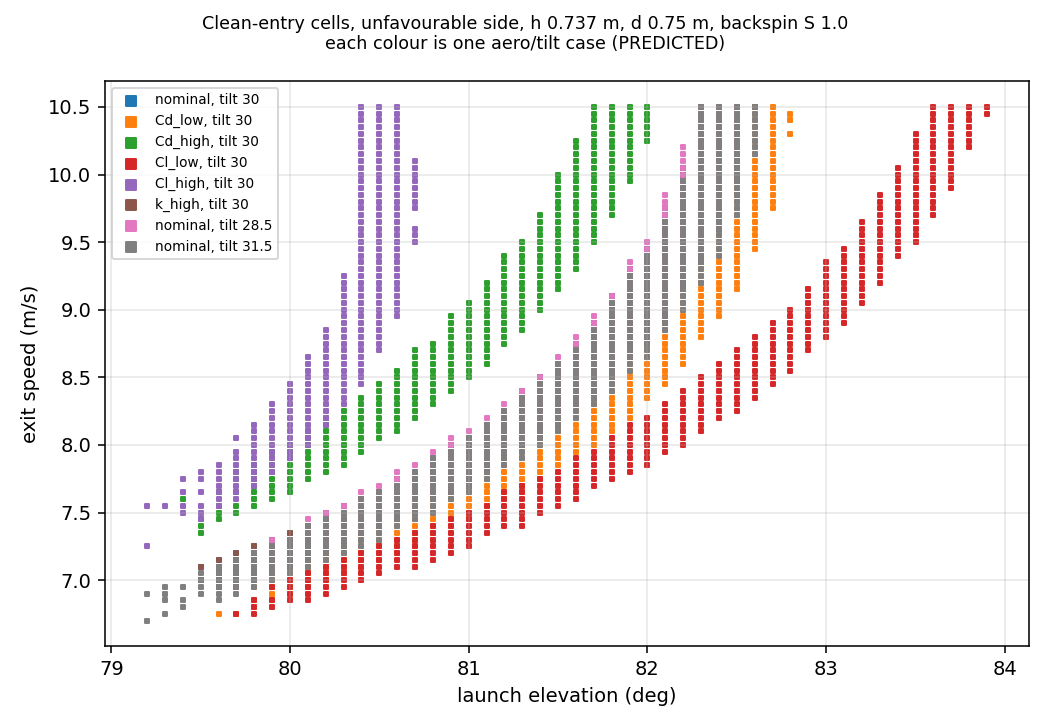
\includegraphics[width=0.9\linewidth]{spec_windows_h737_d075.png}
  \caption{PREDICTED clean-entry cells in the (launch elevation, exit speed) plane for an
    unfavourable-side shot from release height $h=0.737$\,\unit{m}\assumed{} and distance
    $d=0.75$\,\unit{m}\assumed{} with backspin $S=1.0$\assumed. Each colour is one aerodynamic or
    tilt condition from \code{research/params\_lit.json} (nominal, low and high $C_d$, low and high
    lift, fast spin decay) or the tilt bounds $28.80^\circ$\derived{} and $31.77^\circ$\derived{} with
    nominal aerodynamics. The clean bands of the
    different conditions do not overlap in one common cell (Eq.~\eqref{eq:robust_spec-robust}), which
    is why the specification relies on tuning the wheel speed on the field
    (Section~\ref{sec:robust_spec-hood}). All cells are model output, not measurements.}
  \label{fig:spec-windows}
\end{figure}

\section{From windows to requirements: robustness, Monte Carlo and the shooter specification}
\label{sec:robust_spec}

% Source of truth: src/shooter_spec.py (grid, variants, best_square, fixed_elev, describe,
% spec_rows, longest_run, tunable_rows, wheel_rpm, spin_rpm), src/robustness.py (wilson,
% integrate3d, backspin_axis, mc_shots, mc_scenarios, smooth_prob, best_over_hw,
% lateral_factor, wind_drift_sd, position_prob, clean_masks) and src/feasibility.py
% (integrate_batch, evaluate_gate, grid_from_candidates).
% Every worked number below was computed on 2026-10-30 with the system python against the
% repo code. Spec-grid numbers use research/params_lit.json (shooter_spec.py always loads it).
% The Monte Carlo numbers in data/robust_mc.csv and data/robust_map_*.csv were produced with the
% older data/aero_params.json (their CSV headers say so); see the comments in
% Section~\ref{sec:robust_spec-mc}.

The earlier sections give, for one release state, a yes-or-no answer: does the ball enter the
upward-facing CELL of the HIVE cleanly or not?
A shooter, though, is not a single release state.
Its exit speed and its angle scatter from shot to shot, the ball's mass and its aerodynamic
coefficients are only known within assumed, literature-based ranges, and the HIVE itself sits on the field
with a tolerance.
This section turns the yes-or-no windows into numbers a CAD designer can build to.
It goes in five steps:
(i) sample the clean window on a grid;
(ii) find the largest clean square in that grid and read it as a $\pm$ tolerance;
(iii) ask which hood angle stays usable when the aerodynamics change and the team re-tunes only
the wheel speed;
(iv) smooth the window with Gaussian release errors, and run a full three-dimensional Monte Carlo
with per-shot physics, wind and HIVE pose, scored with a Wilson interval;
(v) convert the result into wheel and ball rpm and a CAD card.

All targets at the end of this section are model outputs, so they carry \predicted.
They are design targets to be checked on the field, not measured performance.

Throughout, the frame is the one of Section~\ref{sec:flight}: $x$ is horizontal toward the HIVE,
$y$ is horizontal and sideways, and $z$ points up.
The shot comes from the unfavourable side: the ball has to pass over the roof of the HIVE and then
drop into the CELL, whose mouth faces outward and upward at the tilt angle
$\beta = 30^\circ$\confirmed\ (Competition Manual figure and official CAD).

% ---------------------------------------------------------------------------------------------
\subsection{The clean window on a grid}
\label{sec:robust_spec-grid}

\paragraph{Motivation.}
The flight solver answers ``clean or not'' for one release state.
To talk about tolerances we need that answer on a regular grid of release states, so that
neighbouring cells can be compared.

\paragraph{Release state.}
A shot is released from horizontal distance $d$ (\unit{m}) before the HIVE pivot plane and at
height $h$ (\unit{m}) above the tiles, with exit speed $v$ (\unit{m/s}), elevation angle
$\theta$ (\unit{deg}, above horizontal) and spin parameter $S$ (dimensionless, $S=\omega R/|\vect{v}|$
with ball radius $R$ in \unit{m} and spin rate $\omega$ in \unit{rad/s}).
In two dimensions there is no wind, so the forces depend only on the velocity and the spin, not on
the position.
The solver \code{integrate\_batch} therefore integrates each path once from the origin, giving
$\vect{r}_0(t;v,\theta,S)$, and translates it:
\begin{equation}
  \vect{r}(t;h,d,v,\theta,S) = \vect{r}_0(t;v,\theta,S) + (-d,\; h)^{\mathsf T}.
  \label{eq:robust_spec-translate}
\end{equation}
This is exact because the right-hand side of the equations of motion contains no position
(it depends on the velocity and, through the spin decay, on the time since release only).
One integration serves every $(h,d)$ pair, which is what makes a dense grid affordable.

\paragraph{Clean indicator.}
Let $\vect{n}_{\mathrm{out}}$ be the outward unit normal of the CELL mouth (dimensionless) and let
$c(t)$ (\unit{m}) be the raster clearance between the ball surface and the nearest HIVE part.
Following \code{evaluate\_gate}, a path is clean when it crosses the mouth edge (the gate segment
between the two lips) at a time $t_g$ (\unit{s}), moving inward, without touching anything on the
way in:
\begin{equation}
  M(h,d,v,\theta) =
  \begin{cases}
    1, & \text{if } \exists\, t_g:\ \vect{r}(t_g)\in\text{gate},\ \
         \vect{v}(t_g)\cdot\vect{n}_{\mathrm{out}} < 0,\ \ c_{\min}(t_g) \ge 0, \\
    0, & \text{otherwise,}
  \end{cases}
  \label{eq:robust_spec-mask}
\end{equation}
where $c_{\min}(t_g)=\min_{t_{\mathrm{box}}\le t\le t_g} c(t)$ (\unit{m}) and $t_{\mathrm{box}}$ (\unit{s})
is the time the ball enters the raster box around the HIVE.

\paragraph{Grid.}
The specification grid of \code{shooter\_spec.grid} is
\begin{equation}
  v_i = v_{\min} + i\,\Delta v,\qquad \theta_j = \theta_{\min} + j\,\Delta\theta ,
  \label{eq:robust_spec-grid}
\end{equation}
with $v_{\min}=5.0$\,\unit{m/s}\assumed, $\Delta v = 0.05$\,\unit{m/s}\assumed\ and 111\derived\ speeds up
to 10.5\,\unit{m/s}\assumed; $\theta_{\min}=62^\circ$\assumed, $\Delta\theta=0.1^\circ$\assumed\ and
261\derived\ elevations up to $88^\circ$\assumed.
The release heights are 0.20, 0.35, 0.50, 0.65 and 0.737\,\unit{m}\assumed, and distances run from
0.60\,\unit{m}\assumed\ to 1.75\,\unit{m}\assumed\ in steps of 0.05\,\unit{m}\assumed\ (24\derived\ values).
The spin values are $S\in\{0, 0.5, 1.0, 1.5, -1.0\}$\assumed, where negative $S$ is topspin.

The flight solver returns candidate distances $d_k$ (\unit{m}) at which a path hits the gate.
\code{grid\_from\_candidates} marks a grid distance $d$ clean only if two candidates at consecutive
time samples $k$, $k+1$ of the same path are both clean and bracket it:
\begin{equation}
  M(d) = 1 \iff \exists k:\ M(d_k)=M(d_{k+1})=1,\ \ \min(d_k,d_{k+1}) \le d \le \max(d_k,d_{k+1}).
  \label{eq:robust_spec-dcell}
\end{equation}
This is conservative: a clean point that is isolated between two dirty neighbours is not counted.

\paragraph{Worked example.}
Table~\ref{tab:robust_spec-nclean} lists the number of clean $(v,\theta)$ cells
$N(h,d)=\sum_{i,j}M(h,d,v_i,\theta_j)$ for the nominal aerodynamic set of
\code{research/params\_lit.json}.
At $d\le0.70$\,\unit{m}\assumed\ no cell is clean at the heights
$h=0.50$ to $0.737$\,\unit{m}\assumed: the ball cannot both clear the roof and descend steeply enough
into the mouth from that close.
The count peaks near $d=0.80$\,\unit{m}\predicted\ and then falls slowly with distance.
At $d=0.75$\,\unit{m}\assumed\ the window shrinks with height: 378\predicted\ cells at
$h=0.737$\,\unit{m}\assumed, 286\predicted\ at 0.65\,\unit{m}\assumed\ and 169\predicted\ at
0.50\,\unit{m}\assumed\ (no spin).
For $S=1$ at $h=0.50$\,\unit{m}\assumed\ the cell count at $d=0.75$\,\unit{m}\assumed\ is already
0\predicted.

\begin{table}[htbp]
  \centering
  \caption{Clean cells on the $111\times261$ speed--elevation grid at $h=0.737$\,\unit{m}, nominal
    aerodynamics (\code{research/params\_lit.json}).}
  \label{tab:robust_spec-nclean}
  \begin{tabular}{@{}lrrrrrrr@{}}
    \toprule
    $d$ (\unit{m}) & 0.75 & 0.80 & 0.85 & 0.90 & 1.15 & 1.50 & 1.75 \\
    \midrule
    $N$, $S=0$ & 378\predicted & 457\predicted & 436\predicted & 426\predicted & 359\predicted & 287\predicted & 247\predicted \\
    $N$, $S=1$ & 292\predicted & 412\predicted & 408\predicted & 386\predicted & 335\predicted & 244\predicted & 209\predicted \\
    \bottomrule
  \end{tabular}
\end{table}

Backspin does not make the window larger here: $S=1$ has fewer clean cells than $S=0$ at every
distance in the table.
The case $S=1.5$ gives exactly the same window as $S=1.0$, because the lift coefficient has
already saturated (Section~\ref{sec:flight}): with the nominal set, $C_L = \min(c_1 S, C_{L,\max})$ stops
growing at $S_{\mathrm{sat}} = C_{L,\max}/c_1 = 0.25/0.35 = 0.714$\derived.
More spin above that adds nothing.

\paragraph{Assumptions.}
\begin{itemize}
  \item The 2D model has no wind and no sideways motion; azimuth is added in
    Section~\ref{sec:robust_spec-azimuth}.
  \item A grid cell is a point sample; nothing is claimed about the space between grid points.
  \item The aerodynamic coefficients are assumed ranges based on pickleball and smooth-sphere data,
    not proven bounds and not POLLEN measurements.
  \item The HIVE tilt is the nominal $30^\circ$\confirmed\ unless a variant says otherwise.
\end{itemize}

% ---------------------------------------------------------------------------------------------
\subsection{The largest clean square and the $\pm$ tolerance}
\label{sec:robust_spec-square}

\paragraph{Motivation.}
A shooter set to $(v_c,\theta_c)$ that actually fires anywhere in
$[v_c-\delta_v, v_c+\delta_v]\times[\theta_c-\delta_\theta,\theta_c+\delta_\theta]$ is clean every time
only if that whole box is clean.
The largest all-clean $k\times k$ block of cells is therefore the best repeatability target the
window allows.
\code{best\_square} finds it in $O(N_v N_\theta)$ work per size using a prefix sum.

\paragraph{Prefix sum.}
Let $M_{ij}\in\{0,1\}$ be the mask on the $N_v\times N_\theta$ grid for fixed $(h,d,S)$.
Define the two-dimensional prefix sum (a count, dimensionless)
\begin{equation}
  P_{ij} = \sum_{i'=0}^{i-1}\sum_{j'=0}^{j-1} M_{i'j'},\qquad P_{0j}=P_{i0}=0 .
  \label{eq:robust_spec-prefix}
\end{equation}

\paragraph{Block sum, step by step.}
The number of clean cells in the $k\times k$ block whose lower corner is $(i_0,j_0)$ is
$B_k(i_0,j_0)=\sum_{i=i_0}^{i_0+k-1}\sum_{j=j_0}^{j_0+k-1}M_{ij}$.
The sum $P_{i_0+k,\,j_0+k}$ covers the rectangle $[0,i_0+k)\times[0,j_0+k)$.
Subtracting $P_{i_0,\,j_0+k}$ removes the rows below $i_0$, and subtracting $P_{i_0+k,\,j_0}$ removes the
columns left of $j_0$.
The corner $[0,i_0)\times[0,j_0)$ has now been removed twice, so it is added back once
(inclusion--exclusion):
\begin{equation}
  B_k(i_0,j_0) = P_{i_0+k,\,j_0+k} - P_{i_0,\,j_0+k} - P_{i_0+k,\,j_0} + P_{i_0,\,j_0}.
  \label{eq:robust_spec-block}
\end{equation}
Because each $M_{ij}\le1$, the block is all clean exactly when its count is the largest possible:
\begin{equation}
  \text{block clean} \iff B_k(i_0,j_0) = k^2 .
  \label{eq:robust_spec-allclean}
\end{equation}

\paragraph{Monotone search.}
Every $k\times k$ clean block contains a $(k-1)\times(k-1)$ clean block, so if no block of size $k$
exists, none of a larger size exists either.
The code increases $k$ from 1 and stops at the first size with no hit:
\begin{equation}
  k^\ast = \max\{k:\ \exists (i_0,j_0),\ B_k(i_0,j_0)=k^2\}.
  \label{eq:robust_spec-kstar}
\end{equation}
When several blocks of size $k^\ast$ exist, the code keeps the one whose lower corner is closest (in
index units) to the centroid $(\bar\imath,\bar\jmath)$ of the lower corners of all hits (the same as
comparing block centres, since every centre is the corner shifted by $(k^\ast-1)/2$), which keeps the
choice away from the edge of a cluster:
\begin{equation}
  (i_0,j_0) = \arg\min_{\text{hits}} \Big[\big(i_0-\bar\imath\big)^2
              + \big(j_0-\bar\jmath\big)^2\Big].
  \label{eq:robust_spec-tie}
\end{equation}

\paragraph{Centre and tolerance.}
The $k$ cell centres of the block span $k-1$ grid steps.
The set point is the middle of that span, and the half-span is the tolerance:
\begin{align}
  v_c &= v_{\min} + \Big(i_0+\frac{k^\ast-1}{2}\Big)\Delta v, &
  \theta_c &= \theta_{\min} + \Big(j_0+\frac{k^\ast-1}{2}\Big)\Delta\theta,
  \label{eq:robust_spec-centre}\\
  \delta_v &= \frac{k^\ast-1}{2}\,\Delta v, &
  \delta_\theta &= \frac{k^\ast-1}{2}\,\Delta\theta .
  \label{eq:robust_spec-tol}
\end{align}
Here $v_c$ and $\delta_v$ are in \unit{m/s}, $\theta_c$ and $\delta_\theta$ in degrees.
A single clean cell ($k^\ast=1$) gives a zero tolerance: the set point works only if the shooter is
perfect.

\paragraph{Worked example.}
At $h=0.737$\,\unit{m}\assumed, $d=0.75$\,\unit{m}\assumed\ and $S=0$\assumed, nominal aerodynamics,
the search ends at $k^\ast=3$\predicted\ with $(i_0,j_0)=(70,218)$\predicted.
Then
$v_c = 5.0 + (70+1)(0.05) = 8.55$\,\unit{m/s}\predicted\ and
$\theta_c = 62 + (218+1)(0.1) = 83.9^\circ$\predicted, with
$\delta_v = 1\times0.05 = 0.05$\,\unit{m/s}\derived\ and
$\delta_\theta = 1\times0.1 = 0.10^\circ$\derived.
The smallest raster clearance inside the block is 4.9\,\unit{mm}\predicted.
For $S=0.5$\assumed\ the square is $k^\ast=4$\predicted\ at (9.125\,\unit{m/s}\predicted,
$82.35^\circ$\predicted), above the $8.909$\,\unit{m/s}\predicted\ grip limit of
Section~\ref{sec:launcher:grip} (the search applies no speed cap); for $S=1.0$\assumed\ it is
$k^\ast=4$\predicted\ at (8.875\,\unit{m/s}\predicted, $81.85^\circ$\predicted).
Over every unfavourable-side row of the nominal sweep (nominal aerodynamics, $30^\circ$\confirmed\ tilt)
with $S\in\{0,0.5,1\}$, the square sizes are
$k^\ast=4$ in 14\predicted\ rows, $k^\ast=3$ in 250\predicted, $k^\ast=2$ in 42\predicted,
$k^\ast=1$ in 2\predicted\ and empty in 52\predicted.
No row of it reaches $k^\ast=5$.
So, for the nominal aerodynamics and tilt, $\pm0.075$\,\unit{m/s}\predicted\ and $\pm0.15^\circ$\predicted\
is the widest tolerance the grid admits (a requirement on the shooter, not a measured repeatability).
Only backspin reaches it ($S=0.5$ in 4\predicted\ rows, $S=1.0$ in 10\predicted); the no-spin twin stops
at $k^\ast=3$\predicted, i.e.\ $\pm0.05$\,\unit{m/s}\predicted\ and $\pm0.10^\circ$\predicted.
Single changed conditions can do better: with high drag at the $31.77^\circ$\derived\ tilt
($h=0.737$\,\unit{m}\assumed, $d=0.75$\,\unit{m}\assumed) backspin reaches $k^\ast=5$\predicted\ at
9.25\,\unit{m/s}\predicted, above the grip limit, and the twin $k^\ast=4$\predicted\ at
(8.875\,\unit{m/s}\predicted, $83.35^\circ$\predicted).
Each square is found for one set of coefficients and one tilt; no single setting is clean under
all conditions at once (Section~\ref{sec:robust_spec-hood}).

\paragraph{Assumptions.}
\begin{itemize}
  \item A square block in index space is used; with $\Delta v=0.05$\,\unit{m/s}\assumed\ and
    $\Delta\theta=0.1^\circ$\assumed\ this fixes the aspect ratio of the tolerance box.
  \item Cleanliness is checked only at the cell centres of the block.
  \item One aerodynamic set, one tilt and one $(h,d)$ at a time.
\end{itemize}

% ---------------------------------------------------------------------------------------------
\subsection{Many conditions: the robust intersection and the field-tuned hood}
\label{sec:robust_spec-hood}

\paragraph{Motivation.}
The square above is for the nominal coefficients.
On the field the drag and lift of a real POLLEN, and the HIVE tilt, can be anywhere inside their
bounds.
A fixed hood fixes the elevation angle; the wheel speed is the one thing the team can tune at the
field.
This subsection asks which hood angle leaves a usable speed under every condition.

\paragraph{Conditions.}
A condition $c$ is one aerodynamic variant combined with one HIVE tilt.
\code{shooter\_spec.variants} gives the nominal set and the drag bounds (Cd\_low, Cd\_high); for
$S\ne0$ it adds the lift bounds (Cl\_low, Cl\_high) and fast spin decay (k\_high).
The tilts are $28.80^\circ$\derived, $30^\circ$\confirmed\ and $31.77^\circ$\derived\ (the field
acceptance lip-height tolerance, solved exactly for the tilt).
That gives $3\times3=9$\derived\ conditions for $S=0$ and $6\times3=18$\derived\ for $S\ne0$.
Each condition has its own mask $M_c(v_i,\theta_j)$.

\paragraph{Robust intersection.}
The strictest requirement is a single $(v,\theta)$ that is clean in every condition:
\begin{equation}
  M_{\mathrm{rob}}(v_i,\theta_j) = \prod_{c} M_c(v_i,\theta_j).
  \label{eq:robust_spec-robust}
\end{equation}
On the unfavourable side this mask is empty in every one of the 600\predicted\ rows of
\code{data/spec\_robust.csv}: no single speed and angle works for all drag, lift and tilt bounds at
once.
This is why the specification must rely on field tuning.

\paragraph{Elevation band.}
A real hood angle is set to within $\pm\tau$ (\unit{deg}).
With $n_b=\mathrm{round}(\tau/\Delta\theta)$ (cells), a speed cell is usable at hood index $j$ only if
it is clean at every elevation in the band:
\begin{equation}
  G_c(v_i,j) = \prod_{|j'-j|\le n_b} M_c(v_i,\theta_{j'}),\qquad n_b\le j< N_\theta-n_b .
  \label{eq:robust_spec-band}
\end{equation}

\paragraph{Longest run.}
For fixed $j$, \code{longest\_run} scans $G_c(\cdot,j)$ along the speed axis.
With the run length $L_i = (L_{i-1}+1)\,G_c(v_i,j)$, $L_{-1}=0$, the longest run and its centre (a
speed index, possibly a half integer) are
\begin{equation}
  n_c(j) = \max_i L_i,\qquad
  \hat\imath_c(j) = \arg\max_i L_i - \frac{n_c(j)-1}{2}.
  \label{eq:robust_spec-run}
\end{equation}
The nominal-only fixed-hood value in \code{describe} uses only the nominal condition and picks the $j$
with the longest run (ties broken by the larger worst-case clearance), with set speed
$(v_{\mathrm{lo}}+v_{\mathrm{hi}})/2$ and tolerance $(v_{\mathrm{hi}}-v_{\mathrm{lo}})/2$ over that run.

\paragraph{Field-tuned hood.}
\code{tunable\_rows} lets each condition use its own speed.
The hood is feasible at index $j$ if every condition has at least one usable speed run.
The guaranteed run length is the worst one,
\begin{equation}
  w(j) = \min_c n_c(j),\qquad \text{feasible}\iff w(j)>0 ,
  \label{eq:robust_spec-wmin}
\end{equation}
and the spread of the run centres measures how far the team may have to re-tune,
$\Sigma(j) = \max_c \hat\imath_c(j) - \min_c \hat\imath_c(j)$ (cells; $\Delta v\,\Sigma(j)$ in \unit{m/s}).
The code ranks hood indices by a lexicographic score (run length first, small spread second; the
spread is at most $N_v-1=110$ cells, so the factor 1000 keeps the run length dominant):
\begin{equation}
  j^\ast = \arg\max_j \Big[1000\,w(j) - \Sigma(j)\Big].
  \label{eq:robust_spec-score}
\end{equation}
The reported tuning range and the speed tolerance that every condition keeps at the chosen hood are
\begin{equation}
  v_{\mathrm{tune}}\in\Big[v_{\min}+\Delta v\min_c\hat\imath_c(j^\ast),\
                          v_{\min}+\Delta v\max_c\hat\imath_c(j^\ast)\Big],\qquad
  \delta_{v,\mathrm{tune}} = \frac{w(j^\ast)-1}{2}\,\Delta v .
  \label{eq:robust_spec-tune}
\end{equation}
Note that the masks are not intersected here: Eq.~\eqref{eq:robust_spec-wmin} needs a run to exist in each
condition separately, and the runs may sit at different speeds.
% Code/doc difference: the task wording speaks of masks "intersected over conditions". The code
% (tunable_rows) takes min_c of run lengths with per-condition speeds; the true intersection is
% spec_rows / spec_robust.csv, and it is empty. This text follows the code.

\paragraph{Worked example.}
At $h=0.737$\,\unit{m}\assumed\ and $d=0.75$\,\unit{m}\assumed\ with $\tau=0.2^\circ$\assumed\
($n_b=2$\derived):
\begin{itemize}
  \item No spin: the hood is $\theta_{\mathrm{hood}}=80.9^\circ$\predicted.
    The nine run centres lie between 6.7\,\unit{m/s}\predicted\ (Cd\_low) and
    7.4\,\unit{m/s}\predicted\ (Cd\_high); the nominal-drag centres are
    6.875--6.9\,\unit{m/s}\predicted.
    The worst run is $w=1$\predicted\ cell, so $\delta_{v,\mathrm{tune}}=0$\derived: each condition has
    exactly one tuned speed that works.
  \item Backspin $S\in\{0.5,1.0,1.5\}$: no hood index is feasible at $\tau=0.2^\circ$\assumed.
    With $\tau=0.1^\circ$\assumed\ ($n_b=1$\derived) the code picks $80.4^\circ$\predicted\ for both
    $S=0.5$ and $S=1.0$, with $w=3$\predicted, i.e.\
    $\delta_{v,\mathrm{tune}}=0.05$\,\unit{m/s}\derived.
    The no-spin twin at the same band picks $84.0^\circ$\predicted\ with $w=4$\predicted\
    ($\delta_{v,\mathrm{tune}}=0.075$\,\unit{m/s}\derived).
    Neither search applies the $8.909$\,\unit{m/s}\predicted\ grip limit of
    Section~\ref{sec:launcher:grip}, and both tuning ranges reach above it (to 9.125\,\unit{m/s}\predicted\
    with backspin, 9.575\,\unit{m/s}\predicted\ without).
    With the speeds capped there, backspin keeps $w=2$\predicted\ at $80.3^\circ$\predicted\ and the
    twin $w=3$\predicted\ at $82.0^\circ$\predicted.
  \item With $\tau=0.5^\circ$\assumed\ no row of the sweep is feasible for any spin.
\end{itemize}
Without the band ($\tau=0$), every condition has clean speeds at the backspin hood $80.4^\circ$\predicted\
(conditions of $S=0.5$ and $S=1$ together);
the lowest clean speed per condition ranges from 6.85\,\unit{m/s}\predicted\ to 8.6\,\unit{m/s}\predicted\
(the high-lift set needs the most speed).
For no spin at $80.9^\circ$\predicted\ the union of the nine clean speed sets is
6.6--7.0\,\unit{m/s}\predicted\ and 7.2--7.5\,\unit{m/s}\predicted.
An exit speed range of about 6.5--9.0\,\unit{m/s}\predicted\ therefore contains a clean speed for
every condition at the chosen hood.
The nominal-only fixed hood of \code{describe} at $\tau=0.2^\circ$\assumed\ is $82.8^\circ$\predicted\
for no spin (7.75--7.8\,\unit{m/s}\predicted) and $80.9^\circ$\predicted\ for $S=0.5$
(7.6--7.65\,\unit{m/s}\predicted) and $S=1$ (7.8--7.85\,\unit{m/s}\predicted); at
$\tau=0.5^\circ$\assumed\ it finds none.
At $80.9^\circ$\predicted\ the high-lift conditions of $S=0.5$ and $S=1$ (all three tilts) have no
clean speed even at $\tau=0$, so this nominal-only hood does not carry over to the high lift set.
% Code/doc difference: docs/08_shooter_spec.md says a fixed hood at +-0.2 deg shrinks the window to
% a single 0.05 m/s cell. In the code this holds for S = 0 only; for backspin tunable_rows finds no
% feasible hood at +-0.2 deg (only at +-0.1 deg).
% Code/doc difference: docs/08 "about 81 deg (no spin)" matches the tunable hood 80.9 deg; the
% nominal-only hood02 value for S = 0 is 82.8 deg.

\paragraph{Assumptions.}
\begin{itemize}
  \item The team can re-tune wheel speed at the field but not the hood angle.
  \item The conditions are one-at-a-time changes from the nominal set (drag low/high; for $S\ne0$ also
    lift low/high and fast spin decay) at three tilts, not joint corners and not a measured distribution.
    The floor lift set of Table~\ref{tab:flight-clsets} ($c_1=0.02$\assumed, $C_{L,\max}=0.04$\assumed),
    which \code{research/params\_lit.json} recommends as the pessimistic set, is not included.
  \item Topspin ($S=-1$\assumed) is feasible at $\tau=0.2^\circ$\assumed\ in the sweep
    (for example $82.0^\circ$\predicted, 6.5--7.2\,\unit{m/s}\predicted) but is not the chosen
    configuration.
\end{itemize}

% ---------------------------------------------------------------------------------------------
\subsection{Release errors as a Gaussian blur}
\label{sec:robust_spec-smooth}

\paragraph{Motivation.}
The square and the band treat the tolerance as a hard box.
Real release errors are random, so the right question is the probability of a clean shot when the
shooter aims at a cell.
For independent Gaussian errors this probability is the clean mask blurred by a Gaussian.

\paragraph{Expectation as convolution.}
Let the actual distance, speed and elevation be $d+\delta_d$, $v(1+\varepsilon_v)$ and
$\theta+\delta_\theta$, with $\delta_d\sim\mathcal N(0,\sigma_d^2)$ (\unit{m}),
$\varepsilon_v\sim\mathcal N(0,\sigma_{v,\mathrm{rel}}^2)$ (dimensionless) and
$\delta_\theta\sim\mathcal N(0,\sigma_\theta^2)$ (\unit{deg}), all independent.
The probability of a clean shot is
\begin{equation}
  p(d,v,\theta) = \mathbb E\big[M(d+\delta_d,\ v(1+\varepsilon_v),\ \theta+\delta_\theta)\big].
  \label{eq:robust_spec-expect}
\end{equation}
Near a reference speed $v_{\mathrm{ref}}$ (\unit{m/s}) the speed error is
$v\varepsilon_v\approx v_{\mathrm{ref}}\varepsilon_v$, an additive error of standard deviation
$\sigma_v = \sigma_{v,\mathrm{rel}}v_{\mathrm{ref}}$ (\unit{m/s}).
Writing the expectation as an integral against the product density $\phi$ gives a convolution:
\begin{equation}
  \begin{split}
  p(d,v,\theta) &= \iiint M(d',v',\theta')\,
  \phi_{\sigma_d}(d'-d)\,\phi_{\sigma_v}(v'-v)\,\phi_{\sigma_\theta}(\theta'-\theta)\,
  \mathrm dd'\,\mathrm dv'\,\mathrm d\theta'\\
  &= (M*\phi)(d,v,\theta).
  \end{split}
  \label{eq:robust_spec-conv}
\end{equation}
On the grid, \code{smooth\_prob} evaluates this with \code{scipy.ndimage.gaussian\_filter}, whose
widths are in cells:
\begin{equation}
  s_d = \frac{\sigma_d}{\Delta d},\qquad s_v = \frac{\sigma_{v,\mathrm{rel}}\,v_{\mathrm{ref}}}{\Delta v},\qquad
  s_\theta = \frac{\sigma_\theta}{\Delta\theta}.
  \label{eq:robust_spec-sigcells}
\end{equation}
Cells outside the grid count as dirty (\code{mode="constant"}, value 0) and the kernel is cut at
$3\sigma$.
The speed width is applied piecewise: the mask is filtered three times and each speed row keeps the
result for its nearest reference speed,
\begin{equation}
  v_{\mathrm{ref}}(v_i) = \arg\min_{r\in\{3.5,\,6.0,\,8.5\}} |v_i-r| .
  \label{eq:robust_spec-vref}
\end{equation}
The reference speeds 3.5, 6.0 and 8.5\,\unit{m/s}\assumed\ are code constants.
The best aim at each distance, for a launcher that cannot exceed $v_{\mathrm{cap}}$ (\unit{m/s}), is
\begin{equation}
  P_{\mathrm{kin}}(d) = \max_{v_i\le v_{\mathrm{cap}},\ \theta_j} p(d,v_i,\theta_j).
  \label{eq:robust_spec-pkin}
\end{equation}

\paragraph{Error sets.}
The release error sets of \code{ERR\_SETS} are design assumptions, not measurements.
Listed as $\sigma_{v,\mathrm{rel}}$, $\sigma_\theta$, $\sigma_d$, they are:
tight 0.005\assumed, $0.15^\circ$\assumed, 0.010\,\unit{m}\assumed;
nominal 0.015\assumed, $0.40^\circ$\assumed, 0.025\,\unit{m}\assumed;
loose 0.030\assumed, $0.80^\circ$\assumed, 0.050\,\unit{m}\assumed.
The azimuth and lateral spreads $\sigma_\psi$, $\sigma_y$ are $0.25^\circ$\assumed, 0.010\,\unit{m}\assumed\
(tight), $0.50^\circ$\assumed, 0.025\,\unit{m}\assumed\ (nominal) and $1.00^\circ$\assumed,
0.050\,\unit{m}\assumed\ (loose).

\paragraph{Worked example.}
On the spec grid ($\Delta d = 0.05$\,\unit{m}\assumed) with the nominal errors,
$s_d = 0.025/0.05 = 0.5$\derived\ cells, $s_\theta = 0.40/0.1 = 4.0$\derived\ cells and
$s_v = 0.015\times6.0/0.05 = 1.8$\derived\ cells near 6\,\unit{m/s} (1.05\derived\ near 3.5 and
2.55\derived\ near 8.5\,\unit{m/s}).
At $h=0.737$\,\unit{m}\assumed\ the best smoothed probability with no spin is
0.424\predicted\ at $d=0.75$\,\unit{m}\assumed\ (aim 7.2\,\unit{m/s}\predicted, $81.6^\circ$\predicted),
0.430\predicted\ at $d=0.80$\,\unit{m}\assumed\ (7.05\,\unit{m/s}\predicted, $80.9^\circ$\predicted) and
0.362\predicted\ at $d=1.15$\,\unit{m}\assumed\ (aim 9.1\,\unit{m/s}\predicted, above the grip limit;
0.356\predicted\ with $v_{\mathrm{cap}}=8.909$\,\unit{m/s}\predicted\ of Section~\ref{sec:launcher:grip}).
With $S=1$ it is 0.378\predicted\ at $d=0.75$\,\unit{m}\assumed\ (8.2\,\unit{m/s}\predicted,
$81.3^\circ$\predicted) and 0.412\predicted\ at $d=0.80$\,\unit{m}\assumed\ (7.25\,\unit{m/s}\predicted,
$79.7^\circ$\predicted), below no spin at both distances.
Two points stand out.
First, the smoothed optimum sits near $80$--$82^\circ$, not at the $83.9^\circ$ no-spin square of
Section~\ref{sec:robust_spec-square}: a blur of $4$ cells in elevation rewards the part of the window that is
deep in elevation, while the square rewards the part that is wide in both directions.
Second, even the best aim is clean only about four times in ten with nominal release errors.
On the robustness grid of \code{robustness.py} ($\Delta d=0.01$\,\unit{m}\assumed) the same errors give
$s_d=2.5$\derived\ cells.

\paragraph{Assumptions.}
\begin{itemize}
  \item Errors in $d$, $v$ and $\theta$ are Gaussian, independent and the same for every shot.
  \item The relative speed error is approximated by three fixed additive widths.
  \item The mask is for one aerodynamic condition; physical spread is added in Section~\ref{sec:robust_spec-mc}.
\end{itemize}

% ---------------------------------------------------------------------------------------------
\subsection{Azimuth: why the in-plane distance scales with $\cos\psi$}
\label{sec:robust_spec-azimuth}

\paragraph{Motivation.}
A robot that is not square to the HIVE shoots at an azimuth $\psi$ (\unit{deg} or \unit{rad}) away
from the $x$ axis.
Re-running the 3D solver for every azimuth would be expensive.
\code{clean\_masks} instead reuses the 2D paths and scales their horizontal coordinate and velocity
by $\cos\psi$.
This subsection shows why that is exact in still air.

\paragraph{Rotation about the vertical.}
Let
\begin{equation}
  \mathsf R_\psi = \begin{pmatrix}\cos\psi & -\sin\psi & 0\\ \sin\psi & \cos\psi & 0\\ 0&0&1\end{pmatrix}
  \label{eq:robust_spec-Rz}
\end{equation}
be the rotation by $\psi$ about $\hat{\vect z}$.
It preserves lengths, $|\mathsf R_\psi\vect a| = |\vect a|$, it commutes with the cross product,
$(\mathsf R_\psi\vect a)\times(\mathsf R_\psi\vect b) = \mathsf R_\psi(\vect a\times\vect b)$ (true for
every proper rotation), and it leaves the vertical unchanged, $\mathsf R_\psi\hat{\vect z}=\hat{\vect z}$.

\paragraph{The acceleration is equivariant.}
In still air the 3D acceleration of \code{integrate3d} is
\begin{equation}
  \vect a(\vect v,\vect\omega) = -q\,C_D\,|\vect v|\,\vect v
  + q\,C_L(S)\,|\vect v|^2\,\frac{\vect\omega\times\vect v}{|\vect\omega\times\vect v|} - g\,\hat{\vect z},
  \qquad q=\frac{\rho\pi R^2}{2m},
  \label{eq:robust_spec-acc3d}
\end{equation}
with air density $\rho$ (\unit{kg/m\textsuperscript{3}}), ball mass $m$ (\unit{kg}), drag and lift coefficients
$C_D$, $C_L$ (dimensionless), $q$ in \unit{1/m} and $g$ in \unit{m/s\textsuperscript{2}}.
(The code regularises the two denominators with $\varepsilon=10^{-6}$\assumed; this does not affect the
argument.)
The spin parameter $S=|\vect\omega|R/|\vect v|$ is a ratio of lengths, so it is unchanged by the
rotation.
Applying the three properties term by term:
\begin{equation}
  \vect a(\mathsf R_\psi\vect v,\mathsf R_\psi\vect\omega)
  = -qC_D|\vect v|\,\mathsf R_\psi\vect v
  + qC_L|\vect v|^2\,\frac{\mathsf R_\psi(\vect\omega\times\vect v)}{|\vect\omega\times\vect v|}
  - g\,\mathsf R_\psi\hat{\vect z}
  = \mathsf R_\psi\,\vect a(\vect v,\vect\omega).
  \label{eq:robust_spec-equiv}
\end{equation}
The spin decays as $\vect\omega(t)=\vect\omega_0e^{-kt}$ about a fixed axis, with decay rate
$k$ (\unit{1/s}), so the rotated spin stays the rotated spin at all times.

\paragraph{The backspin axis rotates with the shot.}
The launch direction is $\hat{\vect v}_0 = (\cos\theta\cos\psi,\ \cos\theta\sin\psi,\ \sin\theta)$ and
\code{backspin\_axis} takes the unit vector along $\hat{\vect v}_0\times\hat{\vect z}$:
\begin{equation}
  \begin{split}
  \hat{\vect v}_0\times\hat{\vect z} &= (\cos\theta\sin\psi,\ -\cos\theta\cos\psi,\ 0),\\
  \hat{\vect e}_\omega &= (\sin\psi,\ -\cos\psi,\ 0) = \mathsf R_\psi(0,-1,0)^{\mathsf T}.
  \end{split}
  \label{eq:robust_spec-axis}
\end{equation}
At $\psi=0$ this is $-\hat{\vect y}$, and $(-\hat{\vect y})\times(v_x,0,v_z)=(-v_z,0,v_x)$, which is
the 2D Magnus direction of Section~\ref{sec:flight}.

\paragraph{The path rotates rigidly.}
Let $\vect r_2(t)=(x(t),0,z(t))$ be the 2D path launched at $\psi=0$.
By Eqs.~\eqref{eq:robust_spec-equiv}--\eqref{eq:robust_spec-axis}, $\mathsf R_\psi\vect r_2(t)$ satisfies the same
equation of motion as the 3D path launched at $\psi$, from the rotated initial state.
Solutions of an ODE with a Lipschitz right-hand side are unique, so
\begin{equation}
  \vect r_3(t) = \mathsf R_\psi\,\vect r_2(t) = \big(x(t)\cos\psi,\ x(t)\sin\psi,\ z(t)\big).
  \label{eq:robust_spec-proj}
\end{equation}
The HIVE cross-section does not change along the pivot axis $y$ (inside the CELL width), so only the
$x$--$z$ projection matters for the clean test.
That projection keeps $z$ and scales the horizontal coordinate and velocity:
\begin{equation}
  X(t) = x(t)\cos\psi,\qquad V_X(t) = v_x(t)\cos\psi,\qquad Z(t)=z(t),\qquad V_Z(t)=v_z(t),
  \label{eq:robust_spec-projX}
\end{equation}
which is exactly what \code{clean\_masks} applies before the gate test.
Wind breaks the argument: with $\vect v_r = \vect v-\vect w$ and a fixed wind $\vect w$ (\unit{m/s}),
$\mathsf R_\psi\vect w\ne\vect w$ in general, so the 3D Monte Carlo integrates with wind directly.

\paragraph{Azimuth from the lateral offset.}
A shot aimed at lateral offset $y$ (\unit{m}) from the CELL centre reaches the gate plane at
horizontal distance $d\pm x_g$, where $x_g=0.401$\,\unit{m}\derived\ is the gate position in the HIVE
frame.
The robustness maps use
\begin{equation}
  \psi = \arctan\frac{|y|}{d\pm x_g},\qquad
  s_{\mathrm{eff}} = \min(0.3\tan\psi,\ 0.2)\ \unit{m},
  \label{eq:robust_spec-psi}
\end{equation}
with azimuth bins $0^\circ$ to $60^\circ$\assumed\ in $10^\circ$\assumed\ steps; $s_{\mathrm{eff}}$ is an
assumed effective sideways shift of the mouth seen at an angle (coefficients 0.3\assumed\ and
0.2\,\unit{m}\assumed).

\paragraph{Lateral factor.}
The sideways miss at the gate is $e_y$ (\unit{m}).
An azimuth error $\delta_\psi\sim\mathcal N(0,\sigma_\psi^2)$ (\unit{rad}) over a lever arm
$L=\sqrt{(d\pm x_g)^2+y^2}$ (\unit{m}, the horizontal release-to-gate distance used by
\code{position\_prob}; $L=d+x_g$ for an unfavourable shot with $y=0$) moves the ball by
$L\tan\delta_\psi\approx L\delta_\psi$.
Adding a lateral release error $\sigma_y$ (\unit{m}) and a wind drift $\sigma_{\mathrm{dr}}$ (\unit{m}),
all independent and Gaussian, the variances add:
\begin{equation}
  \sigma_{\mathrm{lat}}^2 = (L\sigma_\psi)^2 + \sigma_y^2 + \sigma_{\mathrm{dr}}^2 .
  \label{eq:robust_spec-latsig}
\end{equation}
The ball fits if $|e_y|<w_{\mathrm{lat}}$, with half-width $w_{\mathrm{lat}}$ (\unit{m}).
For $e_y\sim\mathcal N(0,\sigma_{\mathrm{lat}}^2)$, substituting $u=e/(\sqrt2\sigma_{\mathrm{lat}})$,
\begin{equation}
  \begin{split}
  \Pr(|e_y|<w_{\mathrm{lat}})
  &= \int_{-w_{\mathrm{lat}}}^{w_{\mathrm{lat}}}\frac{e^{-e^2/(2\sigma_{\mathrm{lat}}^2)}}{\sqrt{2\pi}\,\sigma_{\mathrm{lat}}}\,\mathrm de
  = \frac{2}{\sqrt\pi}\int_0^{w_{\mathrm{lat}}/(\sqrt2\sigma_{\mathrm{lat}})}e^{-u^2}\mathrm du\\
  &= \operatorname{erf}\!\Big(\frac{w_{\mathrm{lat}}}{\sqrt2\,\sigma_{\mathrm{lat}}}\Big).
  \end{split}
  \label{eq:robust_spec-erf}
\end{equation}
\code{position\_prob} combines it with the kinematic probability, treating the two as independent:
\begin{equation}
  P_{\mathrm{pos}}(d,\psi) = P_{\mathrm{kin}}(d,\psi)\,\operatorname{erf}\!\Big(\frac{w_{\mathrm{lat}}}{\sqrt2\,\sigma_{\mathrm{lat}}}\Big).
  \label{eq:robust_spec-ppos}
\end{equation}
The code uses $w_{\mathrm{lat}} = 0.10$\,\unit{m}\assumed\ (low), 0.15\,\unit{m}\assumed\ (primary) and
0.2185\,\unit{m}\derived\ (high, the CELL half-width 0.254\,\unit{m}\confirmed\ minus $R$).

\paragraph{Worked example.}
For the 3D path with params\_lit nominal aerodynamics, $v=7.25$\,\unit{m/s}\assumed,
$\theta=79.7^\circ$\assumed, $S=1$\assumed\ and $\psi=30^\circ$\assumed, the backspin axis is
$(0.5,-0.866,0)$\derived.
Comparing \code{integrate3d} with the 2D solution rotated by Eq.~\eqref{eq:robust_spec-proj}, the largest
differences are $1.1\times10^{-7}$\,\unit{m}\predicted\ in $x$, $1.1\times10^{-16}$\,\unit{m}\predicted\ in
$y$ and 0\predicted\ in $z$: the projection is exact to round-off.
On this path the apex is 2.339\,\unit{m}\predicted\ above the release point; there $v_z=0$ but the ball
still moves horizontally at $v_x=0.903$\,\unit{m/s}\predicted, so it is not at rest at the apex.

For the lateral factor take $d=0.81$\,\unit{m}\assumed, so $L=0.81+0.401=1.211$\,\unit{m}\derived, and the
nominal $\sigma_\psi=0.5^\circ=0.00873$\,\unit{rad}\assumed\ and $\sigma_y=0.025$\,\unit{m}\assumed.
Then $L\sigma_\psi=0.0106$\,\unit{m}\derived\ and, without wind,
$\sigma_{\mathrm{lat}}=\sqrt{0.0106^2+0.025^2}=0.0271$\,\unit{m}\derived; the factor is
1.000\derived\ for $w_{\mathrm{lat}}=0.15$\,\unit{m}\assumed.
With the wind drift $\sigma_{\mathrm{dr}}=0.0615$\,\unit{m}\derived\ from \code{wind\_drift\_sd}
(module-default coefficients \code{data/aero\_params.json}; 0.0634\,\unit{m}\derived\ with
\code{research/params\_lit.json}),
$\sigma_{\mathrm{lat}}=0.0672$\,\unit{m}\derived\ and the factor drops to
$\operatorname{erf}(0.15/(\sqrt2\cdot0.0672))=0.974$\derived, or 0.863\derived\ for
$w_{\mathrm{lat}}=0.10$\,\unit{m}\assumed.
Sideways aim is a small loss next to the in-plane window.

\paragraph{Assumptions.}
\begin{itemize}
  \item Still air for the projection; wind enters only through $\sigma_{\mathrm{dr}}$ and the 3D Monte Carlo.
  \item The HIVE section is uniform along the pivot axis across the CELL width.
  \item Lateral and in-plane outcomes are independent in Eq.~\eqref{eq:robust_spec-ppos}.
  \item Azimuth bins stop at $60^\circ$\assumed\ (\code{PSI\_MAX}).
\end{itemize}

% ---------------------------------------------------------------------------------------------
\subsection{Three-dimensional Monte Carlo}
\label{sec:robust_spec-mc}

\paragraph{Motivation.}
The blur of Section~\ref{sec:robust_spec-smooth} covers release errors in one aerodynamic condition.
A real match mixes everything at once: release errors, ball-to-ball spread, unknown coefficients,
air movement and the HIVE pose.
\code{mc\_shots} draws all of these per shot and flies each shot in 3D.

\paragraph{Per-shot sampling.}
Each shot $n$ draws independent standard normals $\varepsilon_{1},\varepsilon_2,\dots\sim\mathcal N(0,1)$.
The release state is
\begin{align}
  v &= v_{\mathrm{aim}}(1+\sigma_{v,\mathrm{rel}}\varepsilon_1)(1+b) - \frac{\partial v}{\partial n_w}\,\Delta n_w\,f,
  \label{eq:robust_spec-mc-v}\\
  \theta &= \theta_{\mathrm{aim}}+\sigma_\theta\varepsilon_2,\qquad \psi = \sigma_\psi\varepsilon_3,
  \label{eq:robust_spec-mc-ang}\\
  \vect r_0 &= \big(-(d+\sigma_d\varepsilon_4),\ \sigma_y\varepsilon_5,\ h+\sigma_h\varepsilon_6\big),
  \label{eq:robust_spec-mc-pos}
\end{align}
where $b$ (dimensionless) is a uniform speed bias used by the battery-sag scenarios,
$\partial v/\partial n_w$ (\unit{m/s} per rpm) is the launcher-curve slope, $\Delta n_w$ (rpm) the
wheel-speed drop after a shot and $f$ a uniform recovery-deficit fraction for the rapid-fire
scenarios; in the nominal scenario $b=f=0$.
The release-height error is $\sigma_h = 0.005$\,\unit{m}\assumed.
The ball and the air are drawn as
\begin{equation}
  \begin{aligned}
    m &= \operatorname{clip}(\bar m+\sigma_m\varepsilon_7,\ m_{\mathrm{lo}},m_{\mathrm{hi}}), &
    R &= \operatorname{clip}(\bar R+\sigma_R\varepsilon_8,\ R_{\mathrm{lo}},R_{\mathrm{hi}}),\\
    C_D &= \bar C_D(1+0.05\,\varepsilon_9), &
    (c_1,C_{L,\max}) &= (\bar c_1,\bar C_{L,\max})(1+0.10\,\varepsilon_{10}),\\
    \vect w &= \sigma_w(\varepsilon_{11},\varepsilon_{12},0), &
    S &\sim\mathcal U(S_{\mathrm{lo}},S_{\mathrm{hi}}),
  \end{aligned}
  \label{eq:robust_spec-mc-phys}
\end{equation}
with $\sigma_m=0.5$\,\unit{g}\assumed, $\sigma_R=0.25$\,\unit{mm}\assumed, the coefficient spreads
5\,\%\assumed\ and 10\,\%\assumed\ (one factor shared by $c_1$ and $C_{L,\max}$, so $S_{\mathrm{sat}}$
does not move), a wind of $\sigma_w=0.30$\,\unit{m/s}\assumed\ per horizontal component held constant
during the shot, and a spin parameter uniform on $[1.03, 1.27]$\predicted\ (the contact model's hood
band); the release-error-only scenario fixes $S=1.0597$\predicted.
The HIVE is drawn per shot with tilt $\beta=\operatorname{clip}(30^\circ+0.75^\circ\varepsilon_{13},\
28.80^\circ, 31.77^\circ)$ (spread $0.75^\circ$\assumed, clipped to the derived tilt bounds), pivot height
$1.11633$\,\unit{m}\confirmed\ with spread 0.005\,\unit{m}\assumed\ clipped to
1.09093--1.14173\,\unit{m}\confirmed\ (the manual's $\pm1$\,in field tolerance), and an $x$ offset of
spread 0.01\,\unit{m}\assumed.
The initial spin is backspin about the rotated axis of Eq.~\eqref{eq:robust_spec-axis}:
\begin{equation}
  \vect\omega_0 = \hat{\vect e}_\omega(\psi)\,\frac{S\,v}{R}.
  \label{eq:robust_spec-mc-omega}
\end{equation}
The path is integrated with Eq.~\eqref{eq:robust_spec-acc3d} using the relative velocity
$\vect v_r=\vect v-\vect w$.

\paragraph{Scoring one shot.}
Where the path (with $x$ measured from the drawn HIVE position) last crosses the gate plane
$x=x_g$ between samples $k$ and $k+1$, the lateral position is interpolated linearly:
\begin{equation}
  y_g = y_k + (y_{k+1}-y_k)\,\frac{x_g-x_k}{x_{k+1}-x_k}.
  \label{eq:robust_spec-yg}
\end{equation}
If $|y_g| > w_{\mathrm{cell}}-R$, with CELL half-width $w_{\mathrm{cell}}=0.254$\,\unit{m}\confirmed,
the shot hits a side wall (or misses when it never crosses the plane).
Otherwise a HIVE with the drawn tilt, pivot height and ball radius, offset sideways by $|y_g|$, runs
\code{classify\_path} on the in-plane path.
The shot counts as clean only if the outcome is \code{clean}.
Out of $n$ shots, $k$ are clean, and the point estimate is
\begin{equation}
  \hat p = \frac{k}{n}.
  \label{eq:robust_spec-phat}
\end{equation}

\paragraph{Worked example.}
The stored run \code{data/robust\_mc.csv} aims at $d=0.81$\,\unit{m}\predicted,
$v=7.25$\,\unit{m/s}\predicted, $\theta=79.7^\circ$\predicted\ with backspin and $n=1500$\assumed\ shots
per scenario.
Its nominal scenario has $k=455$\predicted, $\hat p=0.303$\predicted, Wilson interval
$[0.281, 0.327]$\derived, and a gate-lateral spread of 0.049\,\unit{m}\predicted.
The other scenarios (all at $n=1500$\assumed):
\begin{itemize}
  \item release errors only (fixed physics, no wind): $\hat p=0.362$\predicted;
  \item tight release errors: 0.411\predicted; loose: 0.157\predicted;
  \item wind $\sigma_w=1.0$\,\unit{m/s}\assumed: 0.111\predicted;
  \item true lift at the low or high bound while the aim was tuned for nominal lift:
    0.097\predicted\ and 0.054\predicted; re-tuned for low lift ($\theta=80.7^\circ$\predicted):
    0.325\predicted;
  \item the no-spin twin aimed at $81.4^\circ$\predicted: 0.317\predicted\ $[0.294, 0.341]$\derived;
  \item the favourable side for comparison: 0.996\predicted.
\end{itemize}
The spin and no-spin intervals overlap, so at this aim backspin gives no measurable gain.
Using the wrong lift coefficient costs far more than the release scatter, which is why the
specification relies on tuning at the field.
A fresh run of 400\assumed\ shots with seed 1000\assumed\ and the same code gives
$k=110$\predicted, $\hat p=0.275$\predicted, Wilson $[0.234, 0.321]$\derived; it overlaps the stored
result.
The two most common failures there are the outer roof (147\predicted\ shots) and the floor
(62\predicted).
% Code/doc difference: docs/06_required_vs_achievable.md and the robust_mc / robust_map CSVs were
% produced with data/aero_params.json (older first-pass set). The robustness CLI default is now
% research/params_lit.json, but data/params_lit/ is empty: no params_lit rerun exists. The numbers
% above are the aero_params.json results.
% Code/doc difference: flight.AERO_PARAMS_PATH (module level) still defaults to
% data/aero_params.json unless PM001_AERO_PATH is set, so code that imports robustness without the
% CLI gets the old set. The 400-shot rerun above used that module default to match the CSV.
% Code/doc difference: docs/06 says the mass is clipped to 23.5-26.5 g (aero_params.json); the
% params_lit upper bound is 27.5 g.
These Monte Carlo results were computed with the older first-pass coefficient file
\code{data/aero\_params.json}; a rerun with \code{research/params\_lit.json} has not been made.
The stored file also predates the current scenario list of \code{mc\_scenarios}: it has no no-spin
shots at the backspin aim, and (as \code{data/aero\_params.json} has no floor set) no rows for the
floor lift set.
% The clip above is the current code (fz.TILT_BOUNDS 28.80-31.77); squashed git history cannot show
% which clip produced data/robust_mc.csv.

\paragraph{Assumptions.}
\begin{itemize}
  \item All spreads in Eqs.~\eqref{eq:robust_spec-mc-v}--\eqref{eq:robust_spec-mc-phys} are assumed, independent and
    Gaussian or uniform; none is measured on the robot.
  \item The wind is constant during one shot and horizontal.
  \item The aerodynamic coefficients are assumed literature-based ranges, not proven bounds and not
    POLLEN measurements.
  \item Shots are independent trials, which Section~\ref{sec:robust_spec-wilson} needs.
\end{itemize}

% ---------------------------------------------------------------------------------------------
\subsection{How sure is a success rate? The Wilson interval}
\label{sec:robust_spec-wilson}

\paragraph{Motivation.}
A rate of $k$ clean shots out of $n$ is itself random.
The simple interval $\hat p\pm z\sqrt{\hat p(1-\hat p)/n}$ fails badly for small $n$ or for
$\hat p$ near 0 or 1: for one clean shot out of one it gives $[1,1]$.
\code{wilson} uses the score interval instead, which is the right tool for field tests.

\paragraph{Derivation.}
For $n$ independent shots with true probability $p$, $k$ is binomial, and for moderate $n$
\begin{equation}
  \frac{\hat p-p}{\sqrt{p(1-p)/n}}\approx\mathcal N(0,1).
  \label{eq:robust_spec-wilson-z}
\end{equation}
The Wilson interval is the set of $p$ for which this score is within $\pm z$, where
$z=\Phi^{-1}(0.975)=1.959964$\derived\ for 95\,\%.
Note that the variance uses the unknown $p$, not $\hat p$.
The boundary satisfies
\begin{equation}
  (\hat p-p)^2 = \frac{z^2}{n}\,p(1-p).
  \label{eq:robust_spec-wilson-quad}
\end{equation}
Expanding both sides and collecting powers of $p$ gives a quadratic:
\begin{equation}
  \Big(1+\frac{z^2}{n}\Big)p^2 - \Big(2\hat p+\frac{z^2}{n}\Big)p + \hat p^2 = 0 .
  \label{eq:robust_spec-wilson-poly}
\end{equation}
Its discriminant simplifies as
\begin{equation}
  \Big(2\hat p+\frac{z^2}{n}\Big)^2 - 4\Big(1+\frac{z^2}{n}\Big)\hat p^2
  = \frac{4z^2}{n}\hat p(1-\hat p) + \frac{z^4}{n^2}
  = 4z^2\Big(\frac{\hat p(1-\hat p)}{n}+\frac{z^2}{4n^2}\Big),
  \label{eq:robust_spec-wilson-disc}
\end{equation}
and the two roots, divided top and bottom by 2, are the interval:
\begin{equation}
  p_\pm = \frac{\hat p + \dfrac{z^2}{2n} \pm z\sqrt{\dfrac{\hat p(1-\hat p)}{n}+\dfrac{z^2}{4n^2}}}{1+\dfrac{z^2}{n}} .
  \label{eq:robust_spec-wilson}
\end{equation}
The code clips both ends to $[0,1]$.
The centre $(\hat p+z^2/2n)/(1+z^2/n)$ is pulled toward $1/2$, and the width never collapses to
zero, even at $\hat p = 0$ or 1.

\paragraph{Worked example.}
For $k=455$\predicted\ of $n=1500$\assumed: $\hat p=0.3033$\derived, $z^2/n=0.00256$\derived, and
Eq.~\eqref{eq:robust_spec-wilson} gives $[0.2806, 0.3271]$\derived.
For $\hat p = 0.5$ the half-width is 0.263\derived\ at $n=10$, 0.201\derived\ at $n=20$,
0.096\derived\ at $n=100$ and 0.025\derived\ at $n=1500$.
One clean shot out of one gives $[0.207, 1]$\derived: a single shot proves only that the clean rate is
probably above about one in five, and says nothing about repeatability.
Zero clean shots out of 20 still allows a rate up to 0.161\derived.
A field test that should separate a 30\,\% shooter from a 50\,\% one therefore needs on the order of
100 shots per setting, not a handful.

\paragraph{Assumptions.}
\begin{itemize}
  \item Shots are independent with a common probability (no warm-up drift).
  \item The normal approximation in Eq.~\eqref{eq:robust_spec-wilson-z}; the Wilson form keeps good coverage
    down to small $n$.
\end{itemize}

% ---------------------------------------------------------------------------------------------
\subsection{From exit speed to wheel and ball rpm}
\label{sec:robust_spec-rpm}

\paragraph{Motivation.}
The CAD designer chooses a motor and gear ratio, so the speed requirement must be stated as a wheel
rpm, and the spin requirement as a ball rpm.

\paragraph{Wheel rpm.}
A wheel of diameter $D$ (\unit{m}) turning at $n_w$ (rpm) has surface speed
$u=\pi D\,n_w/60$ (\unit{m/s}).
The exit speed of the ball is a fraction $r=v/u$ (dimensionless) of the surface speed.
Solving for the wheel speed:
\begin{equation}
  n_w = \frac{60\,v}{r\,\pi D}.
  \label{eq:robust_spec-wheel}
\end{equation}
This is \code{wheel\_rpm}.
The ratio $r$ is not universal.
With a single powered wheel against a fixed hood the ball rolls on the hood, and the simple
rolling picture gives $r=1/2$; slip, compression and a moving upper roller change it.
The code tabulates $r\in\{0.25, 0.30, 0.42, 0.50\}$\assumed\ (grade C), and the contact model of
the previous section is the place where $r$ is predicted.

\paragraph{Ball rpm.}
From $S=\omega R/v$, the spin rate is $\omega=Sv/R$ (\unit{rad/s}); converting with
$1\,\text{rev}=2\pi$\,\unit{rad} and $1\,\text{min}=60$\,\unit{s},
\begin{equation}
  n_b = \frac{S\,v}{R}\cdot\frac{60}{2\pi}.
  \label{eq:robust_spec-spinrpm}
\end{equation}
This is \code{spin\_rpm}.
There is no point in asking for spin far above $S_{\mathrm{sat}}$: the lift coefficient saturates
and $S=1.5$ gives the same window as $S=1.0$ (Section~\ref{sec:robust_spec-grid}).

\paragraph{Worked example.}
With $D=0.098$\,\unit{m}\userval\ and $R=0.0355$\,\unit{m}\confirmed\ (the manual's ball diameter of
about 7.1\,\unit{cm}):
\begin{itemize}
  \item $v=6.5$\,\unit{m/s}\predicted:
    $n_w = 60\times6.5/(0.25\,\pi\,0.098) = 5067$\derived\ rpm at $r=0.25$\assumed, and
    4222\derived, 3016\derived, 2533\derived\ rpm at $r=0.30$, 0.42, 0.50.
  \item $v=9.0$\,\unit{m/s}\predicted: 7016\derived, 5847\derived, 4176\derived, 3508\derived\ rpm.
  \item $v=7.0$\,\unit{m/s}\predicted: 5457\derived, 4547\derived, 3248\derived, 2728\derived\ rpm.
  \item Ball spin: $S=0.5$\assumed\ at 6.5\,\unit{m/s} is
    $n_b=0.5\times6.5/0.0355\times60/(2\pi)=874$\derived\ rpm; $S=1$\assumed\ at 7.0\,\unit{m/s} is
    1883\derived\ rpm and at 9.0\,\unit{m/s} is 2421\derived\ rpm.
\end{itemize}
The full exit-speed band 6.5--9.0\,\unit{m/s} therefore asks for anything from about 2500 to 7000 rpm
at the wheel depending on $r$; measuring $r$ on the first prototype narrows this to one gear choice.

\paragraph{Assumptions.}
\begin{itemize}
  \item $r$ is constant over the speed range for a given shooter build.
  \item The wheel speed does not drop during the shot (the drop is a Monte Carlo scenario, Eq.~\eqref{eq:robust_spec-mc-v}).
\end{itemize}

% ---------------------------------------------------------------------------------------------
\subsection{The shooter specification card}
\label{sec:robust_spec-card}

\paragraph{Motivation.}
The final step collects the results above into the few numbers the CAD designer needs.
Each target traces back to an equation and a worked example of this section.
All of them are model outputs.

\begin{table}[htbp]
  \centering
  \caption{CAD-card targets for the unfavourable-side shot (single powered 98\,mm wheel, fixed hood).
    All targets are model predictions to be confirmed on the field.}
  \label{tab:robust_spec-card}
  \begin{tabular}{@{}p{0.24\linewidth}p{0.26\linewidth}p{0.42\linewidth}@{}}
    \toprule
    Quantity & Target & Where it comes from \\
    \midrule
    Release height $h$ & 0.65--0.737\,\unit{m}\predicted & Table~\ref{tab:robust_spec-nclean}; window shrinks below 0.65\,\unit{m}\predicted \\
    Distance $d$ & 0.75--0.85\,\unit{m}\predicted & no clean cell at $d\le0.70$\,\unit{m}\predicted; peak near 0.80\,\unit{m}\predicted \\
    Hood angle, no spin & about $81^\circ$\predicted & Eq.~\eqref{eq:robust_spec-score}: $80.9^\circ$\predicted\ at $\tau=0.2^\circ$\assumed \\
    Hood angle, backspin & about $80.4^\circ$\predicted & Eq.~\eqref{eq:robust_spec-score} at $\tau=0.1^\circ$\assumed, $S=0.5$\assumed\ and $1.0$\assumed\ ($80.3^\circ$\predicted\ with speeds capped at the grip limit) \\
    Exit speed range & 6.5--9.0\,\unit{m/s}\predicted & every condition has a clean speed (Sec.~\ref{sec:robust_spec-hood}) \\
    Speed repeatability & $\pm0.075$\,\unit{m/s}\predicted\ with backspin, $\pm0.05$\,\unit{m/s}\predicted\ without & Eq.~\eqref{eq:robust_spec-tol}, $k^\ast=4$\predicted\ with backspin, $k^\ast=3$\predicted\ for the no-spin twin (nominal aerodynamics) \\
    Angle repeatability & $\pm0.15^\circ$\predicted\ with backspin, $\pm0.10^\circ$\predicted\ without & Eq.~\eqref{eq:robust_spec-tol}, as for the speed \\
    Wheel speed & about 2500--7000 rpm\predicted & Eq.~\eqref{eq:robust_spec-wheel}, depends on $r$ \\
    \bottomrule
  \end{tabular}
\end{table}

\paragraph{How to read the card.}
\begin{itemize}
  \item \emph{Height and distance.}
    The window opens at $d\approx0.75$\,\unit{m}\predicted\ and is largest near 0.80\,\unit{m}\predicted;
    beyond 0.85\,\unit{m} it shrinks slowly.
    Lower release heights shrink it quickly (Table~\ref{tab:robust_spec-nclean} and the $h$ comparison in
    Section~\ref{sec:robust_spec-grid}).
  \item \emph{Hood angle.}
    The hood is chosen so that, for every drag, lift and tilt condition, some tuned wheel speed is clean
    (Eq.~\eqref{eq:robust_spec-wmin}).
    The backspin hood is slightly flatter than the no-spin hood, but backspin does not enlarge the
    window and its hood needs a tighter angle tolerance ($\pm0.1^\circ$ instead of $\pm0.2^\circ$).
  \item \emph{Exit speed.}
    The range is a tuning range, not a tolerance: the team sets one speed at the field and keeps it.
  \item \emph{Repeatability.}
    The $\pm0.075$\,\unit{m/s}\predicted\ and $\pm0.15^\circ$\predicted\ figures are the largest clean
    square of the nominal sweep (nominal coefficients, $30^\circ$\confirmed\ tilt;
    Section~\ref{sec:robust_spec-square}), and only backspin reaches them; the no-spin twin reaches
    $\pm0.05$\,\unit{m/s}\predicted\ and $\pm0.10^\circ$\predicted.
    Each square is found for one set of coefficients and one tilt.
    They are a target for shot-to-shot scatter, roughly the tight release set of the Monte Carlo
    ($\sigma_\theta=0.15^\circ$\assumed), which raises the modelled clean rate from 0.30\predicted\ to
    0.41\predicted.
    They are not a guarantee of clean entry under every condition.
\end{itemize}
% Code/doc difference: docs/08 puts the repeatability (no spin +-0.05 m/s and +-0.1 deg, backspin
% +-0.075 m/s and +-0.15 deg) on the card next to the ~81 deg hood. In the code these are the
% nominal-aero best squares at h = 0.737 m, d = 0.75 m, tilt 30 deg: S = 0 k*=3 at (8.55 m/s,
% 83.9 deg), S = 0.5 k*=4 at (9.125 m/s, 82.35 deg, above the 8.909 m/s cap), S = 1 k*=4 at
% (8.875 m/s, 81.85 deg); none is at the ~81 deg hood and none is robust over conditions. At the
% field-tuned no-spin hood (tunable_rows, tau = 0.2 deg) the guaranteed speed tolerance is 0.
% Code/doc difference: docs/08 gives the backspin hood as about 80.5-81.5 deg (band centre). The
% field-tuned hood at +-0.1 deg is 80.4 deg (80.3 deg with speeds capped at 8.909 m/s). The
% nominal-only hood (fixed_elev at +-0.2 deg) is 80.9 deg, where the Cl_high conditions have no clean
% speed. At +-0.2 deg the field-tuned search finds no backspin hood.

\paragraph{Assumptions.}
\begin{itemize}
  \item A single powered wheel with a fixed hood (an optional passive upper roller changes $r$ and
    the spin, not the geometry of the window).
  \item The coefficient ranges of \code{research/params\_lit.json} for the spec grid; the Monte Carlo
    rates were computed with \code{data/aero\_params.json}.
  \item No claim here is based on a single test shot; field confirmation needs a Wilson interval
    from many shots (Section~\ref{sec:robust_spec-wilson}).
\end{itemize}

% =============================================================================================
\section{Whole-field model, live solver and missing effects}
\label{sec:field}

Sections~\ref{sec:geometry}--\ref{sec:robust_spec} treat one shot straight down the HIVE tipping
plane. This section describes how the same flight model is used for a release point anywhere on the
field (the explorer's Robot view, \code{viz/explorer/solver.js}, with a Python copy in
\code{src/}), which effects were added on top of it, and which effects are still missing. Every
window here is model output\predicted{} with the literature aerodynamics\assumed; none of it is a
hit rate.

% ---------------------------------------------------------------------------------------------
\subsection{Whole-field oblique model}
\label{sec:field-oblique}

The release point is $(x,y)$ in the field frame of the HIVE section: $x$ along the shot axis with the
pivot plane at $x=0$, the far (unfavourable) side at $x<0$, and the up-cell gate centre at
$(x_g,0)$ with $x_g=0.401$\,\unit{m}\derived. The shot is aimed at the gate centre. With
$d=|x|$ the distance to the pivot plane,
\begin{equation}
  L_h=\begin{cases} d+x_g & \text{far side},\\ \max(d-x_g,\,10^{-3}\,\text{m}) & \text{near side},\end{cases}
  \qquad \psi=\arctan\frac{|y|}{L_h},
  \label{eq:field-psi}
\end{equation}
where $\psi$ is the bearing off the HIVE centre line\derived. The ball flies in the vertical plane of
that bearing with its spin axis perpendicular to it, so there is no sideways Magnus force. Its
in-plane path is the planar path of Section~\ref{sec:flight} with the horizontal coordinate and
velocity projected on the shot axis,
\begin{equation}
  X_{\text{axis}}(t)=X(t)\cos\psi,\qquad V_{X,\text{axis}}(t)=V_X(t)\cos\psi,
  \label{eq:field-proj}
\end{equation}
and the lateral offset of the ball centre from the cell centre line is
$s(t)=(x_g-x_{\text{axis}}(t))\tan\psi$. The projection is exact for walls extruded along $y$ and
still air. Bearings above $60^\circ$\assumed{} are flagged as extrapolated.

% ---------------------------------------------------------------------------------------------
\subsection{The 3D cell: side walls and pentagon roof}
\label{sec:field-cell3d}

The precomputed maps use the centre section at one assumed lateral offset per bearing and do not
model the side walls. The live solver instead tests the ball-centre path $(x,y,z)$ against the cell
as 3D faces inflated by $R=0.0355$\,\unit{m}\confirmed: the centre section extruded across the cell,
side walls at $\pm0.254$\,\unit{m}\confirmed{} with inner face, rim and outer face, wall thickness
$0.0508$\,\unit{m}\assumed, and a pentagon roof whose ridge drops linearly towards the side walls
(from the opening profile $0.3556\to0.19329$\,\unit{m} over $0.254$\,\unit{m}\derived). The
clearance is the exact segment-to-polygon distance minus $R$. A shot is clean when the centre enters
the cell interior before any face comes closer than $R$.

At $\psi=0$ with the ridge off the 3D test reproduces the section test exactly (2500 shots per side).
With the ridge on it is slightly stricter on the centre line, because the roof is lower off it. Off
the centre line the 3D cell is usually more permissive than the old single-offset section: at
$d=1.0$\,\unit{m}, $h=0.5$\,\unit{m}, $S=1.0$ the far-side clean grid cells go from $306$ to $301$ at
$\psi=0$, from $212$ to $309$ at $20^\circ$ and from $164$ to $362$ at $40^\circ$\predicted{} (no-spin
twin $348\to346$, $253\to347$, $186\to401$\predicted). These are counts on a coarse search grid, not
probabilities.

% ---------------------------------------------------------------------------------------------
\subsection{Live solver: knife-edge and tolerant minima}
\label{sec:field-solver}

For a continuous release point and height the solver flies a coarse grid (exit speed $2$--$16$\,\unit{m/s}
in $0.1$\,\unit{m/s} steps, hood angle in $0.1^\circ$ far-side or $0.25^\circ$ near-side steps) and then
refines near the minima. It reports two kinds of minimum:
\begin{itemize}
  \item \textbf{Knife edge} (\code{minRpm}, \code{minAngle}): the lowest clean exit speed or hood angle the
    search found. These are grazing shots. Their clearance is typically $0$--$0.5$\,\unit{mm}\predicted, and the
    value moves with the resolution because the window edge carries about $0.1^\circ$ of path-sampling noise
    at the $2$\,\unit{ms} step. They are shown, but a robot must not be set there.
  \item \textbf{Tolerant} (\code{minRpmTol}, \code{minAngleTol}): the lowest speed whose continuous clean
    hood-angle run is at least $0.2^\circ$\assumed{} wide, and the lowest hood angle whose continuous clean
    speed run is at least $0.1$\,\unit{m/s}\assumed{} wide, with clearance $\ge2$\,\unit{mm}\assumed{} at every
    sample. The most forgiving shot is the centre of the largest all-clean square on the search grid.
\end{itemize}
Every result is solved twice: with the chosen backspin and as the no-spin twin ($S=0$, no Magnus
term), with the same air and drag settings. The fused integrate-and-classify fast path is checked
against the reference integrator and classifier for equal class and clearance to $10^{-12}$\,\unit{m}.

At the explorer's default robot spot ($x=-1.0$, $y=0.2$\,\unit{m}\userval, $h=0.737$\,\unit{m}\userval,
$\psi=8.1^\circ$\derived, $S=1.0$\assumed, $v/u=0.42$\assumed, nominal aerodynamics) the solver gives
\begin{center}
\begin{tabular}{@{}lcc@{}}
  \toprule
  & backspin $S=1.0$ & no-spin twin $S=0$ \\
  \midrule
  knife-edge min.\ rpm & $2677$\,rpm at $71.74^\circ$\predicted{} & $2682$\,rpm at $72.86^\circ$\predicted \\
  tolerant min.\ rpm & $2784$\,rpm at $73.30^\circ$\predicted{} & $2784$\,rpm at $74.47^\circ$\predicted \\
  tolerant min.\ hood angle & $75.80^\circ$ at $3023$\,rpm\predicted{} & $77.30^\circ$ at $3034$\,rpm\predicted \\
  most forgiving & $4269$\,rpm at $80.8^\circ$\predicted{} & $4872$\,rpm at $84.7^\circ$\predicted \\
  \bottomrule
\end{tabular}
\end{center}
The rpm values are derived from the exit speed with the assumed grip and a $98$\,\unit{mm}\userval{}
wheel. The knife-edge clearance at the minimum rpm is $0.63$\,\unit{mm}\predicted. At this spot backspin
does not lower the tolerant minimum wheel speed; it lowers the hood angle at that speed by about
$1.2^\circ$\predicted. More spin is not always better: the lift saturates (Section~\ref{sec:flight}).

% ---------------------------------------------------------------------------------------------
\subsection{Robot and turret view}
\label{sec:field-robot}

The Robot view places a $0.457$\,\unit{m}\confirmed{} robot anywhere on the field at any heading. The
release point is the robot centre at the chosen height\assumed, and a turret aims at the cell centre
exactly\assumed. The page reports the turret yaw relative to the robot front and, if the chosen turret
travel ($360^\circ$, $\pm180^\circ$, $\pm90^\circ$, $\pm45^\circ$ or fixed) cannot reach that yaw, how far
to turn the robot. Poses inside the A-frame base are illegal; the second HIVE is only flagged as an
obstacle. The recommended setting is the most forgiving shot, unless it needs more exit speed than the
grip limit below. In that case the lowest tolerant wheel speed is recommended. At the default spot the most forgiving
shot ($4269$\,rpm, about $9.2$\,\unit{m/s}\predicted) is above the limit, so the page recommends
$2784$\,rpm at $73.3^\circ$\predicted{} (twin $2784$\,rpm at $74.5^\circ$\predicted).

% ---------------------------------------------------------------------------------------------
\subsection{Venue air, drag options, drafts and the grip limit}
\label{sec:field-options}

These were added from the ranked list in \code{research/MISSING\_EFFECTS.md} because they need no new
measurement. Python (\code{src/air.py}, \code{src/feasibility.py}) and JavaScript (\code{physics.js},
\code{solver.js}) carry the same formulas. Tests compare trajectories from the two at
$2\times10^{-6}$ relative, which is the float32 storage limit.

\paragraph{Air density.} Simplified CIPM-2007 with a Magnus-form vapour pressure and a US Standard
Atmosphere pressure from altitude,
\begin{equation}
  \rho=\frac{p-0.378\,e}{R_d\,T},\quad e=\phi\,611.2\exp\frac{17.62\,t}{243.12+t},\quad
  p=101325\,(1-2.25577\times10^{-5}\,z)^{5.25588},
  \label{eq:field-rho}
\end{equation}
with $R_d=287.06$\,\unit{J/(kg\,K)}, $t$ in \unit{$^\circ$C}, $T=t+273.15$, humidity $\phi$ and altitude
$z$ in \unit{m} (user inputs). Viscosity follows Sutherland's law. Still air at $20^\circ$C,
$101.325$\,\unit{kPa}, dry gives $\rho=1.2041$\,\unit{kg/m\textsuperscript{3}}\derived{} and
$\nu=1.506\times10^{-5}$\,\unit{m$^2$/s}\derived. This is now the live solver's default instead of the
rounded $1.20$\assumed{} used by the precomputed maps. At the default spot the change moves the tolerant
minimum from $2793$\,rpm at $73.43^\circ$ to $2784$\,rpm at $73.30^\circ$\predicted. The twin stays at
$2784$\,rpm at $74.47^\circ$\predicted{} to the precision shown.

\paragraph{Drag options.} $C_d$ stays the constant literature value by default. Two alternatives are
available. The first is the smooth-sphere correlation $C_d(\mathrm{Re})$ of Morrison (2013), a reference
curve for a ball without holes and not a POLLEN fact. The second is a what-if partial drag crisis that
falls from the constant $C_d$ to $0.33$\assumed{} with a smoothstep between $\mathrm{Re}=3\times10^4$ and
$5\times10^4$\assumed. Backspin can add drag:
\begin{equation}
  C_d\leftarrow C_d+\Delta C_d\,\min(S/0.6,\,1),\qquad \Delta C_d\in\{0,\,0.08,\,0.18\}\assumed .
  \label{eq:field-spindrag}
\end{equation}
The no-spin twin has $S=0$ and never gets this term.

\paragraph{Draft.} A steady draft $\vect{w}=(w_\parallel,w_z)$ in the shot plane (user input) enters
through the relative velocity $\vect{v}_{\text{rel}}=\vect{v}-\vect{w}$. Drag, Magnus force and $S$ all
use it. A sideways part is an option on the 3D path (Section~\ref{sec:field-move}).

\paragraph{Grip limit.} An answer that needs an exit speed above $8.9$\,\unit{m/s}\predicted{}
(the hood launcher model of Section~\ref{sec:launcher}) is flagged, not removed. Above that speed,
$v/u$ and $S$ are uncertain.

\paragraph{Effect at the default spot} (tolerant minimum rpm and its hood angle, twin in brackets; all
\predicted):
\begin{center}
\begin{tabular}{@{}lll@{}}
  \toprule
  option & backspin $S=1.0$ & twin $S=0$ \\
  \midrule
  still air (default) & $2784$\,rpm, $73.30^\circ$ & $2784$\,rpm, $74.47^\circ$ \\
  Morrison $C_d(\mathrm{Re})$ & $2775$\,rpm, $73.64^\circ$ & $2765$\,rpm \\
  what-if drag drop & as still air ($\mathrm{Re}<3\times10^4$ here) & as still air \\
  spin drag $\Delta C_d=0.18$ & $2821$\,rpm, $72.98^\circ$ & $2784$\,rpm (no term) \\
  tail draft $0.3$\,\unit{m/s} & $2803$\,rpm, $73.84^\circ$ & $2784$\,rpm, $74.8^\circ$ \\
  updraft $0.3$\,\unit{m/s} & $2793$\,rpm, $73.84^\circ$ & $2765$\,rpm \\
  altitude $1600$\,\unit{m} ($\rho=0.9925$\derived) & $2775$\,rpm, $73.77^\circ$ & $2765$\,rpm, $74.61^\circ$ \\
  \bottomrule
\end{tabular}
\end{center}
No tolerant minimum at this spot is grip-limited. Each option moves the hood angle by up to about
$0.5^\circ$\predicted, which is wider than the $0.2^\circ$\assumed{} tolerance. A venue therefore needs
its own aim check.

% ---------------------------------------------------------------------------------------------
\subsection{Shooting on the move, hit chance and lift options}
\label{sec:field-move}

These options come from the same ranked list (\code{research/MISSING\_EFFECTS.md}, build-next 2a--2f). All
are off by default, so the default answer above is unchanged. Python (\code{src/robustness.py},
\code{src/air.py}, \code{src/flight.py}) and JavaScript (\code{solver.js}, \code{physics.js}) agree on
launch states to $10^{-12}$, on 3D paths to $10^{-9}$ relative and on every Monte Carlo count
(\code{tests/test\_move.py}, \code{tests/js\_move\_check.js}).

\paragraph{Moving robot.} The robot's ground velocity at the exit point is
$\vect{v}_r=a\,\hat{\vect{u}}+c\,\hat{\vect{n}}+\omega_z\hat{\vect{z}}\times\vect{r}_{\text{exit}}$,
with $\hat{\vect{u}}$ the horizontal aim direction, $\hat{\vect{n}}=\hat{\vect{z}}\times\hat{\vect{u}}$, and the
speeds $a$, $c$ and turn rate $\omega_z$ user inputs (field-frame $v_x$, $v_y$ are also accepted). The ball
leaves with
\begin{equation}
  \vect{v}_0=\vect{v}_{\text{shooter}}(v,\ \theta_e)+\vect{v}_r,\qquad \theta_e=\theta_{\text{hood}}+\delta_0,
  \label{eq:field-move}
\end{equation}
where $\delta_0$ is an exit-angle offset (\assumed, default $0$). With lead on (default) the shooter turns so the
sideways part of $\vect{v}_0$ cancels, which needs $|\vect{v}_r\cdot\hat{\vect{n}}|\le v\cos\theta_e$. The
backspin axis is horizontal and normal to the shooter direction, plus $\omega_z$ about the vertical; the
no-spin twin has no backspin. The flight is then 3D in the 3D cell, with a sideways draft allowed. The solver
also reports how far the centre of the clean run moves per $0.1$\,m/s toward the goal and sideways.

\paragraph{Hit chance.} At one setting the solver fires $n=1000$ shots per aero set (lift low, nominal and
high) with ASSUMED Gaussian launch scatter: speed $1.5\,\%$, elevation $0.40^\circ$, heading $0.50^\circ$
($1\sigma$, the nominal set of Section~\ref{sec:robust_spec-mc}). All sets and the twin use the same seeded
draws. The result is $k/n$ with a Wilson $95\,\%$ interval (Section~\ref{sec:robust_spec-wilson}). It is a
model probability under assumed scatter, not a measured repeatability. At the default spot and the recommended
$2784$\,rpm, $73.3^\circ$: nominal $0.124$ $[0.105,\,0.146]$, lift low $0.092$, lift high $0.074$; the twin
at its own setting ($2784$\,rpm, $74.47^\circ$) about $0.13$ (all \predicted). Backspin does not raise the
chance here.

\paragraph{Lift options.} Gyro-correct spin ratio $S_\perp=|\vect{\omega}\times\vect{v}_{\text{rel}}|R/
|\vect{v}_{\text{rel}}|^2$ on the 3D path (equal to $S$ for pure backspin, tested). A user table $C_l(S)$,
linear between points and flat after the last. Reverse Magnus: when $\mathrm{Re}<4.6\times10^4$ and
$S<0.5$ the lift blends (smoothstep near both bounds) to $-C_{l,\text{rev}}\min(S/0.1,1)$, $C_{l,\text{rev}}\in[0,0.1]$\assumed{} (smooth-sphere
data of Kim et al.\ 2014 and Kray et al.\ 2012, not POLLEN).

\paragraph{Effective mass.} $\varepsilon=(0.5+\phi)\rho V/m$ with $\phi\in[0,1]$\assumed{} the share of the
air inside the ball that moves with it, and
$\dot{\vect{v}}=(\vect{F}_{\text{aero}}/m+\vect{g})/(1+\varepsilon)$. For POLLEN
$\varepsilon=0.0045$ to $0.0136$\derived. Default $\varepsilon=0$.

\paragraph{Effect at the default spot} (tolerant minimum rpm and hood angle; \predicted):
\begin{center}
\begin{tabular}{@{}lll@{}}
  \toprule
  option & backspin $S=1.0$ & no-spin twin \\
  \midrule
  none (default) & $2784$\,rpm, $73.30^\circ$ & $2784$\,rpm, $74.47^\circ$ \\
  moving, all speeds $0$ & same & same \\
  $0.5$\,m/s toward the goal & $2738$\,rpm, $78.09^\circ$ & $2719$\,rpm, $79.01^\circ$ \\
  $0.3$\,m/s sideways, lead & $2812$\,rpm, $73.41^\circ$ & $2784$\,rpm, $74.15^\circ$ \\
  $0.3$\,m/s sideways, no lead & no clean shot & no clean shot \\
  turning $90^\circ$/s & $2793$\,rpm, $73.42^\circ$ & as default \\
  $\delta_0=+1^\circ$ & $2784$\,rpm, $72.30^\circ$ & $2784$\,rpm, $73.47^\circ$ \\
  sideways draft $0.3$\,m/s & $2803$\,rpm, $73.54^\circ$ & $2793$\,rpm, $74.61^\circ$ \\
  $C_l$ table $(0.5,0.2),(1.5,0.35)$ & $2803$\,rpm, $73.25^\circ$ & as default \\
  $\phi=1$ & $2765$\,rpm, $73.34^\circ$ & $2756$\,rpm, $74.36^\circ$ \\
  \bottomrule
\end{tabular}
\end{center}
Driving toward the goal moves the hood angle by about $1^\circ$ per $0.1$\,m/s\predicted, several times the
ASSUMED aim tolerance. Sideways motion with lead halves the backspin window (315 to 158 clean pairs, twin 364
to 347), because the spin axis follows the turned shooter. Reverse Magnus does not act here ($S=1$).

% ---------------------------------------------------------------------------------------------
\subsection{Hit-chance guidance and the measurement protocol}
\label{sec:field-chance}

\paragraph{Best-chance setting.} The lowest-rpm setting above sits near the edge of the clean window, so
the page now recommends the clean setting with the highest model chance to go in instead
(\code{solver.js} \code{bestChance}, replayed in \code{src/robustness.py} \code{best\_chance}). The
candidates are clean cells inside the PREDICTED grip limit ($8.9$\,m/s), ranked by their share of clean
neighbours under a Gaussian with the scatter as $\sigma$ and picked at least one $\sigma$ apart (up to $24$),
plus the tolerant minima. Stage~1 scores each with $64$ shots per air set; at most $5$ whose pooled Wilson
upper bound reaches the best lower bound go to stage~2 with $400$ shots. All candidates in a stage see the
same seeded draws (common random numbers). The winner is scored again on $1000$ fresh shots per air set, so
the reported chance is not biased by the selection. The score is the mean over the three air sets (lift low,
nominal, high), equal weight\assumed. The no-spin twin is searched on its own grid, and one scatter source at a
time names the one that matters most.

\paragraph{Default spot} ($x=-1.0$, $y=0.2$\,m, $h=0.737$\,m\userval, $S=1.0$\userval, grip $0.42$\assumed,
scatter $1.5\,\%$, $0.40^\circ$, $0.50^\circ$\assumed; all chances \predicted, Wilson $95\,\%$ ranges):
\begin{center}
\begin{tabular}{@{}lllll@{}}
  \toprule
  setting & lift low & nominal & lift high & mean \\
  \midrule
  best chance, $3062$\,rpm\derived, $76.2^\circ$ & $0.207$ & $0.295$ $[0.268,\,0.324]$ & $0.064$ & $0.189$ \\
  lowest rpm, $2784$\,rpm\derived, $73.3^\circ$ & $0.092$ & $0.124$ $[0.105,\,0.146]$ & $0.074$ & $0.097$ \\
  no-spin twin at its best, $3851$\,rpm\derived, $82.1^\circ$ & \multicolumn{3}{l}{$0.375$ $[0.346,\,0.405]$ (no lift: one set)} & $0.375$ \\
  no-spin twin at its lowest rpm, $2784$\,rpm, $74.47^\circ$ & \multicolumn{3}{l}{$0.132$ $[0.112,\,0.154]$} & $0.132$ \\
  \bottomrule
\end{tabular}
\end{center}
Here the hood angle is the scatter source that matters most for both shots: with only one source on, the
nominal chance is $0.46$ (speed only), $0.40$ (angle only) and $1.00$ (aim only)\predicted; for the twin
$0.74$, $0.44$ and $1.00$\predicted. At $3\,\%$ speed scatter\userval{} the best setting moves to $3341$\,rpm,
$78.0^\circ$ (nominal $0.258$), speed matters most, and the twin's best is $3990$\,rpm, $82.6^\circ$ ($0.290$)
(all \predicted). At this spot the no-spin twin has the higher chance: more spin is not always better. Over the
lift range the backspin chance moves by a factor of almost five ($0.064$ to $0.295$), so the measured $C_l$
decides whether backspin helps here at all.

\paragraph{What the chance is not.} It is a model probability under ASSUMED scatter and ASSUMED air sets, not
a measured repeatability. It becomes a prediction a team can test only after the scatter itself is measured
(the standard deviation of exit speed and elevation over about $20$ shots at one setting, logged with wheel
speed and battery voltage) and the hit rate is counted with a Wilson interval from many shots
(Section~\ref{sec:robust_spec-wilson}).

\paragraph{Measurement protocol.} \code{docs/MEASURE.md} and the browser kit \code{viz/measure/measure.html}
(linked from the explorer) turn the two largest unknowns into numbers with one phone camera at
$240$\,fps or faster. The ball centre is clicked frame by frame and the track is fitted with the same RK4
flight model as \code{physics.js} (Python \code{src/fit\_aero.py} agrees with the page to $5\times10^{-9}$).
\begin{itemize}
  \item \textbf{Drop test} (no launcher, no spin): $C_d$ at zero spin. With one $4$\,m drop and $4$\,mm click
    noise the $95\,\%$ error is about $\pm0.008$, and about $\pm0.085$ from $1.5$\,m\derived.
  \item \textbf{Twin test:} shot~A with no spin gives $v_0$, the launch angle and $C_d$; shot~B, the same
    setting with backspin, holds A's $C_d$ and gives $C_l$ beside its no-spin twin. On synthetic
    \code{physics.js} tracks (truth ASSUMED, $C_d=0.50$, $C_l=0.25$) one pair gives sd $0.008$ in $C_d$ and
    $0.010$ in $C_l$ at $4$\,mm noise and $0.7$\,s tracked\derived. These are synthetic checks, not POLLEN data.
  \item \textbf{Length scale.} The scale bar is the largest error: $+1\,\%$ in scale moves $C_l$ by about
    $19\,\%$\derived. Shot~A also fits the scale against gravity (sd about $0.3\,\%$\derived), and the fit can
    use either scale.
  \item \textbf{Exit speed and spin:} wheel rpm with the video gives the grip $v/u$; counting turns of a
    striped ball gives $S$ at the first tracked frame.
\end{itemize}
The results go into the explorer's Advanced settings (nearest air preset and grip), and the best-chance search
then runs on measured rather than assumed inputs. Until then every chance above stays a model prediction.

% ---------------------------------------------------------------------------------------------
\subsection{Missing effects and how to measure them}
\label{sec:field-missing}

\code{research/MISSING\_EFFECTS.md} ranks 32 effects by how far they move the answer. The largest ones
that are still not in the model, or are in it only as bracket sets, need measurements rather than code:
\begin{center}
\begin{tabular}{@{}p{0.36\linewidth}p{0.58\linewidth}@{}}
  \toprule
  effect & how to measure \\
  \midrule
  Spin lift level $C_l(S)$ (slope and cap) & side video at 240--480 fps, wheel above vs below at equal rpm, taped-hole ball (T1) \\
  Drag level $C_d$ & the same flight video and a drop test (T1) \\
  Grip-limited exit speed, slip $v/u$, ball squeeze & exit video with a wheel encoder (T2); mass, diameter, squeeze (T0/T4) \\
  Hood angle $\ne$ exit angle, exit scatter & exit video over a hood-angle sweep (T2) \\
  Knuckle force on a low-spin holed ball & shot scatter with and without spin (T1) \\
  Exit skew and spin-axis tilt (sideways error) & axle alignment check; spin axis from video \\
  Balls and NECTAR in the cell, restitution, TIP mid-volley & drop tests on skin, rib and NECTAR; cell tests (T5/T6) \\
  Effective mass (an ASSUMED option only) & absorbed by tuning to real shots; mass and volume (T0) \\
  Flywheel droop, battery; real scatter while moving & burst tests with encoder and voltage logs; shots on the move \\
  Venue drafts and air state & air speed at robot height, temperature, humidity, station pressure \\
  \bottomrule
\end{tabular}
\end{center}
Until those numbers exist, the model's job is to say which measurement changes the answer most. It
does not predict a scoring rate.

% =============================================================================================
\section{Backspin against the no-spin twin over the whole field}
\label{sec:svt}

Section~\ref{sec:field-chance} compared the best backspin setting with the no-spin twin at one spot. This
section repeats that comparison at every legal pose of a coarse field grid (code \code{src/spin\_vs\_twin.py},
data \code{data/spin\_vs\_twin.csv}, notes \code{research/SPIN\_VS\_TWIN.md}). Every chance is a model
probability\predicted{} under ASSUMED launch scatter and ASSUMED air sets. It is not a hit rate. The twin is
a yardstick, not a design. The one-wheel hood always spins the ball: $S$ runs from $1.029$\predicted{} to
$1.274$\predicted{} over the parameter box of Section~\ref{sec:launcher:Sband}, and falls below $1$ only with
a fast feeder. A shooter without spin would be a different mechanism. ``Twin $>$ spin'' therefore means that
backspin gives no gain in this model, not that a no-spin shooter should be built.

% ---------------------------------------------------------------------------------------------
\subsection{Grid, searches and verdict}
\label{sec:svt-method}

\paragraph{Grid.} The release points are $x\in\{\pm0.65,\pm0.95,\pm1.25,\pm1.55\}$\,\unit{m}\assumed{} in the
field frame of Section~\ref{sec:field-oblique} ($x<0$ is the far, unfavourable side; $x>0$ the near,
favourable side) and $y$ from
$-1.2$\assumed{} to $2.0$\,\unit{m}\assumed{} in steps of $0.4$\,\unit{m}\assumed. The release heights are
$h\in\{0.35,\,0.5,\,0.737\}$\,\unit{m}\assumed{} and the backspin values $S\in\{0.5,\,1.0,\,1.5\}$\assumed.
Of the $216$\derived{} poses $(x,y,h)$, $144$\derived{} are scored: $84$\derived{} on the unfavourable side
and $60$\derived{} on the favourable side. Of the other $72$\derived, $48$\derived{} put the
$0.457$\,\unit{m}\confirmed{} robot into a wall or the A-frame base, $15$\derived{} have a bearing $\psi$
(Eq.~\eqref{eq:field-psi}) above $60^\circ$\assumed{}, which the model flags as extrapolated, and
$9$\derived{} lie outside the exported tables.

\paragraph{Searches.} At each pose, three kinds of search run the best-chance procedure of
Section~\ref{sec:field-chance}. The candidates are clean settings inside the $8.9$\,\unit{m/s}\predicted{}
grip limit: up to $24$ grid settings, plus the tolerant lowest-rpm and lowest-hood settings and the most
forgiving one (Section~\ref{sec:field-solver}), $17$\derived{} to $27$\derived{} per search here. Each search
scores every candidate with $64$ shots, takes at most $5$ on to $400$ shots, and scores the winner on $1000$
fresh shots (seed $20261031$, common random numbers).
\begin{itemize}
  \item \textbf{Twin:} $S=0$, no lift, on its own clean grid.
  \item \textbf{Robust}$(S)$: one setting from the nominal set's clean grid, scored over the three lift sets
    pooled with equal weight\assumed{} and reported per set. This is the setting a team would pick without
    knowing the lift.
  \item \textbf{Tuned}$(S,L)$: the best setting for lift set $L$ alone, from that set's clean grid. This is
    the setting a team would pick after the lift has been measured.
\end{itemize}
The twin and every backspin winner at a pose are scored on the same fresh draws, so each pair is matched.

The lift sets are low, nominal and high from Table~\ref{tab:flight-clsets}. Every shot uses
$C_d=0.5$\assumed{} and $k=0.03$\,\unit{1/s}\assumed. The launch scatter is $1.5\,\%$\assumed{} in exit speed,
$0.40^\circ$\assumed{} in elevation and $0.50^\circ$\assumed{} in heading ($1\sigma$), with no spin scatter.
A shot counts only if it enters cleanly; bounce-ins are not scored.

\paragraph{Verdict.} Let $[\ell_s,u_s]$ and $[\ell_t,u_t]$ be the Wilson $95\,\%$ intervals
(Section~\ref{sec:robust_spec-wilson}) of the backspin and twin chances at one pose. Then
\begin{equation}
  \text{verdict}=\begin{cases}
    \text{spin} > \text{twin}, & \ell_s>u_t,\\
    \text{twin} > \text{spin}, & \ell_t>u_s,\\
    \text{unclear}, & \text{otherwise (the intervals overlap)}.
  \end{cases}
  \label{eq:svt-verdict}
\end{equation}
Near $p=0.35$\predicted{} with $n=1000$ the half-width of each interval is about $0.03$\derived, so a verdict
needs a gap of about $0.06$\derived. The matched difference is $\Delta p=p_s-p_t$ on the same draws.

% ---------------------------------------------------------------------------------------------
\subsection{Results}
\label{sec:svt-results}

Table~\ref{tab:svt-unfav} gives the unfavourable side at $S=1.0$, and Fig.~\ref{fig:svt} shows every pose
there. No row has the verdict spin $>$ twin: not on either side, nor for any $S$, search or lift set
($0$\predicted{} of $2592$\derived{} rows).

\begin{table}[htbp]
  \centering
  \caption{Unfavourable side, $84$\derived{} scored poses, $S=1.0$. The $S=1.5$ rows are identical
    (Section~\ref{sec:svt-sat}). The table gives the medians over the poses of the backspin and twin chances and
    of $\Delta p$, the verdict counts of Eq.~\eqref{eq:svt-verdict}, and the cost of not knowing the lift (tuned
    minus robust at the same pose, median $[\min,\max]$). All values are \predicted, in percent or percentage
    points (pp).}
  \label{tab:svt-unfav}
  \small
  \begin{tabular}{@{}llrrrrrl@{}}
    \toprule
    search & lift set & backspin (\%) & twin (\%) & $\Delta p$ (pp) & twin $>$ spin & unclear
      & tuned $-$ robust (pp) \\
    \midrule
    robust & low     & 16.0 & 35.2 & $-20.4$ & 84 & 0  & \\
    robust & nominal & 28.4 & 35.2 & $-8.1$  & 61 & 23 & \\
    robust & high    & 4.4  & 35.2 & $-31.4$ & 84 & 0  & \\
    \addlinespace
    tuned  & low     & 35.7 & 35.2 & $-0.3$  & 0  & 84 & $20.1$ $[14.3,\,28.4]$ \\
    tuned  & nominal & 35.3 & 35.2 & $-0.5$  & 0  & 84 & $7.3$ $[0.0,\,14.4]$ \\
    tuned  & high    & 34.4 & 35.2 & $-1.0$  & 0  & 84 & $30.1$ $[21.7,\,45.4]$ \\
    \bottomrule
  \end{tabular}
\end{table}

\begin{figure}[tbp]
  \centering
  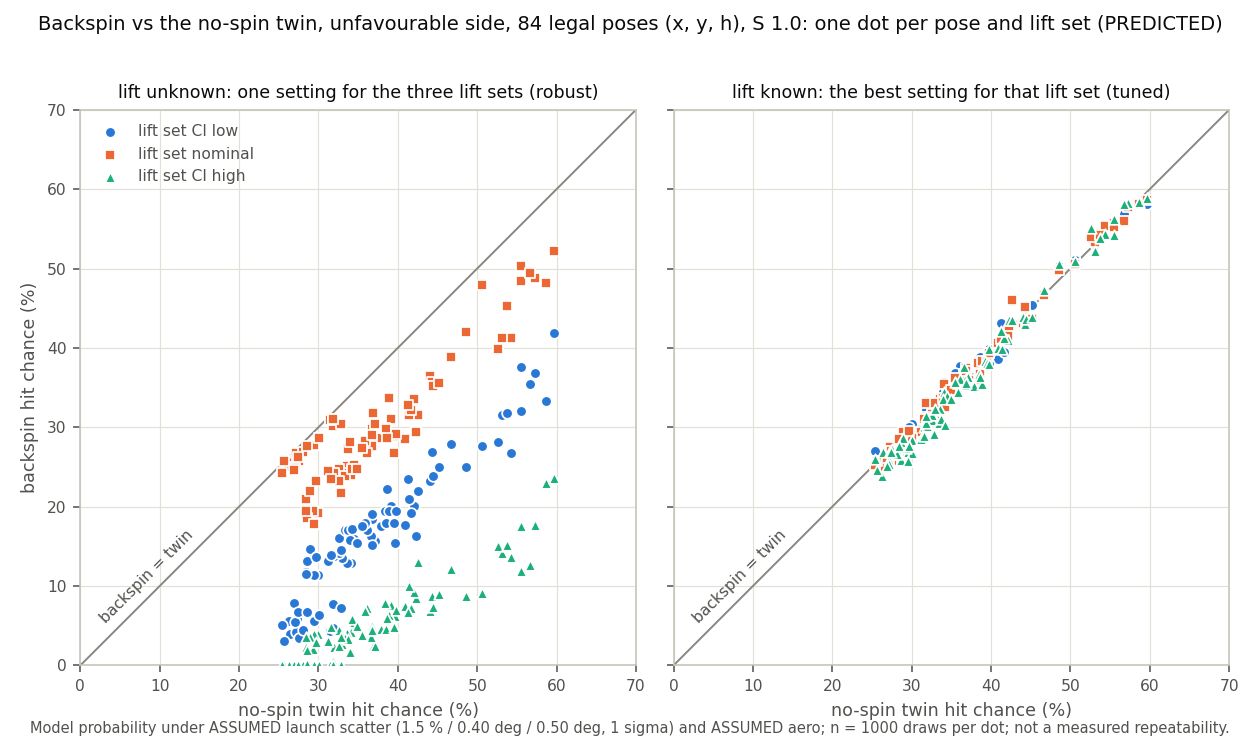
\includegraphics[width=\linewidth]{spin_vs_twin.png}
  \caption{Backspin chance against the twin's chance at every scored unfavourable-side pose, $S=1.0$ (model
    output \predicted{} under ASSUMED scatter and air sets). Left: robust, one setting for all three lift sets
    (the lift unknown). Right: tuned, the setting for the true lift set. Colour and marker give the lift set. A
    dot on the diagonal means backspin $=$ twin. Data: \code{data/spin\_vs\_twin.csv}.}
  \label{fig:svt}
\end{figure}

\paragraph{Lift known: level with the twin.} Tuned backspin and the twin are level at all $84$\derived{}
unfavourable-side poses, for every lift set. The medians are $34.4$\predicted{} to $35.7\,\%$\predicted{}
against $35.2\,\%$\predicted. At $S=1.0$ the median $\Delta p$ is $-0.3$\predicted, $-0.5$\predicted{} and
$-1.0$\,pp\predicted{} for the low, nominal and high sets, with a full range of $-3.9$\predicted{} to
$+3.4$\,pp\predicted. Backspin is lower at $51$\predicted, $62$\predicted{} and $65$\predicted{} of the $84$
poses. All poses use the same seeded draws, so these counts are not independent tests. The lean is also much
smaller than the half-width of each interval, so the model does not resolve it.

\paragraph{Lift unknown: below the twin.} One setting for all three lift sets puts backspin clearly below the
twin at $84$\predicted, $61$\predicted{} and $84$\predicted{} of the $84$ poses. Robust backspin reaches
$50\,\%$ at $2$\predicted{} poses (nominal set only), the twin at $11$\predicted. This is the cost of not
knowing the lift, $7.3$\predicted{} to $30.1$\,pp\predicted{} at the median (last column of
Table~\ref{tab:svt-unfav}). It is not an advantage of a ball without spin. The robust search pools only the
lift uncertainty, the twin has no lift to pool, and $C_d$ has the same fixed value for both shots. If $C_d$ were
uncertain too, both shots would pay for it; that case was not run. Tuning on the real ball, or measuring its
lift, removes the cost in the model.

\paragraph{Favourable side.} Both shots enter almost always: medians $99.7$\predicted{} to
$99.8\,\%$\predicted{} against $99.8\,\%$\predicted. Every pose is unclear except $3$\predicted{} in robust
$S=0.5$ with the high set, where the twin is clearly higher ($97.9$\predicted{} to $98.6\,\%$\predicted{}
against $99.8$\predicted{} to $99.9\,\%$\predicted).

\paragraph{Where on the unfavourable side.} The twin's chance ranges from $25.4$\predicted{} to
$59.7\,\%$\predicted{} over the $84$ poses. All $11$\predicted{} poses where it reaches $50\,\%$ lie on the
line $x=-0.65$\,\unit{m}\assumed, at bearings $|\psi|=37.3^\circ$\derived{} to $56.7^\circ$\derived. There the
twin gives $50.6$\predicted{} to $59.7\,\%$\predicted{} and tuned backspin $50.6$\predicted{} to
$58.9\,\%$\predicted, unclear at every pose and for every set. The robust shot is clearly below the twin at
$31$\predicted{} of the $33$ pose and set pairs. In the robust nominal case the twin is clearly higher at
$15$\predicted, $19$\predicted{} and $27$\predicted{} of $28$ poses for $h=0.35$\assumed, $0.5$\assumed{}
and $0.737$\,\unit{m}\assumed.

\paragraph{Settings.} The median unfavourable-side winners at $S=1.0$ are: robust $7.20$\,\unit{m/s}\predicted{}
at $74.8^\circ$\predicted{} ($3341$\,rpm\derived); tuned $8.40$\predicted{} to $8.50$\,\unit{m/s}\predicted{}
at $76.0^\circ$\predicted{} to $78.2^\circ$\predicted{} ($3898$\derived{} to $3944$\,rpm\derived); twin
$8.50$\,\unit{m/s}\predicted{} at $79.6^\circ$\predicted{} ($3944$\,rpm\derived). The rpm values use the grip
$v/u=0.42$\assumed{} and the $98$\,\unit{mm}\userval{} wheel.

% ---------------------------------------------------------------------------------------------
\subsection{Why \texorpdfstring{$S=1.5$}{S = 1.5} gives the same answer as \texorpdfstring{$S=1.0$}{S = 1.0}}
\label{sec:svt-sat}

Section~\ref{sec:flight-lift} showed that two launches which stay above saturation for the whole flight follow
the same path (Eq.~\eqref{eq:flight-FM-sat}). In this sweep the flights already meet that condition at
$S_0=1.0$:
\begin{enumerate}
  \item In still air $\vect{v}_{\mathrm{rel}}=\vect{v}$ and $\vect{F}_M\perp\vect{v}$, so the lift does no
    work and $\frac{\mathrm{d}}{\mathrm{d}t}\bigl(\tfrac12|\vect{v}|^2+gz\bigr)=\vect{v}\cdot\vect{F}_D/m\le0$,
    with $\vect{F}_D$ the drag force.
  \item A shot is followed from release ($z=h$) until it falls back below $z=h+z_s$. Here
    $z_s=\min(0.4\,\text{m},\,z_{\text{cell}}-0.05\,\text{m}-h)=0.4$\,\unit{m}\derived{} for every $h$ of the
    grid, with $z_{\text{cell}}=1.252$\,\unit{m}\derived{} the lowest point of the CELL. So $z\ge h$ on the whole
    path, and $|\vect{v}(t)|\le v_0$.
  \item With Eq.~\eqref{eq:flight-S-t} and $t\le t_{\max}=3.0$\,\unit{s}\assumed, the integration limit,
    \begin{equation}
      S(t)\;\ge\;S_0\,e^{-kt}\;\ge\;S_0\,e^{-kt_{\max}}=0.914\,S_0.
      \label{eq:svt-bound}
    \end{equation}
  \item $S_{\mathrm{sat}}=0.75$\derived, $0.714$\derived{} and $0.50$\derived{} for the low, nominal and high
    sets. So for $S_0\ge0.75/0.914=0.82$\derived{} all three sets stay at their cap for the whole flight.
  \item $C_d$ does not depend on spin, the launch scatter has no spin part, and the score depends on the path
    alone. So $S_0=1.0$ and $S_0=1.5$ give the same hits on the same draws.
\end{enumerate}
The sweep confirms this. All $576$\derived{} searches at $S=1.5$ equal their $S=1.0$ partners (setting, counts
and interval), so $864$\derived{} of $864$ rows are the same. The high set starts at its cap when $S_0=0.5$,
and its tuned rows at $S=0.5$ equal the $S=1.0$ rows at $144$\derived{} of $144$ poses. Most other $S=0.5$ rows
differ, because there the lift stays below its cap for part of the flight. At $S=0.5$ the unfavourable-side
tuned medians are $34.4$\predicted{} to $34.8\,\%$\predicted, and the robust medians are $18.0$\predicted,
$30.6$\predicted{} and $1.0\,\%$\predicted{} (low, nominal, high), against $35.2\,\%$\predicted{} for the
twin. Neither $S$ beats the twin. In this model
more spin is therefore not better, and above $S_0\approx0.82$\derived{} it changes nothing. As
Section~\ref{sec:flight-lift} stresses, the cap is a model assumption. A real perforated ball may keep gaining
lift, show a dip or gain drag with spin, and then $S$ would matter again, in either direction.

% ---------------------------------------------------------------------------------------------
\subsection{Limits and what would change the answer}
\label{sec:svt-limits}

\begin{itemize}
  \item \textbf{Air sets.} The air sets are literature bounds, not POLLEN data, and no lift of POLLEN has been
    measured yet. $C_d$ is fixed for both shots. The spin-drag option of Eq.~\eqref{eq:field-spindrag}, off by
    default, would act on the backspin shot only and was not run.
  \item \textbf{Scatter.} The scatter is assumed and is the same for both shots, with no spin scatter. On a ball
    whose lift keeps rising with $S$, spin scatter would hit the backspin shot only.
  \item \textbf{Clean entry only.} Bounce-ins and bounce-outs are not scored, and Section~\ref{sec:contact}
    finds that backspin can lower retention after a contact.
  \item \textbf{Grid.} The grid is coarse. Spots closer than $x=-0.65$\,\unit{m}\assumed{} are not sampled. At
    $33$\derived{} of the $84$ unfavourable-side poses the straight line to the aim point crosses the other
    HIVE in plan; it is flagged but not modelled as an obstacle (a high ball can pass above it).
  \item \textbf{Exact tuning.} Still air and a robot at rest are assumed. The tuned search knows the true lift
    set exactly, which tuning by test shots on a field does not.
\end{itemize}
Four measurements would change the answer: POLLEN's $C_l(S)$ and $C_d$ from the twin test of
Section~\ref{sec:field-chance}, the real exit $S$ of the hood, the real launch scatter including spin, and the
retention after a contact. For the verdict to become spin $>$ twin, a gap of about $6$\,pp\derived{} is needed
near $p=0.35$\predicted. The largest tuned gap in this sweep is $+3.7$\,pp\predicted{} at $S=0.5$\assumed{}
(nominal set, $(x,y,h)=(-0.95,\,-1.2,\,0.737)$\,\unit{m}\assumed: $46.3\,\%$\predicted{} against the twin's
$42.6\,\%$\predicted, unclear). At $S=1.0$ it is $+3.4$\,pp\predicted{} at the same pose and set
($46.0\,\%$\predicted{} against $42.6\,\%$\predicted).


% =============================================================================================
\section{Limitations and what to measure}
\label{sec:limits}

Every result above is a prediction of a model whose most important inputs have never been measured
on POLLEN. The model is useful for deciding \emph{what to build and what to measure first}; it is not
evidence that the shot works. The prototype test plan in \code{docs/07\_test\_plan.md} turns the list
below into concrete tests with pass and fail lines.

\begin{itemize}
  \item \textbf{Shot scatter.} The clean window on the unfavourable side is narrow: with the nominal
    coefficients and the $30^\circ$\confirmed{} tilt, the largest clean square found is about
    $\pm0.075$\,\unit{m/s}\predicted{} by $\pm0.15^\circ$\predicted{} with backspin
    ($S=0.5$\assumed{} or $1.0$\assumed) and $\pm0.05$\,\unit{m/s}\predicted{} by
    $\pm0.10^\circ$\predicted{} for the no-spin twin. These are tolerances the shooter must hold, not
    a measured repeatability. Whether a real shooter holds them is the deciding question for
    hypothesis (A); its scatter must be measured as the standard deviation of exit speed and elevation
    over many shots at one setting, with the wheel-speed sag from rapid fire and battery voltage
    logged alongside.
  \item \textbf{The ratio $v/u$.} The exit speed as a fraction of the wheel surface speed depends on
    the hood friction, the compression and the ball; the model does not treat $v=u/2$ as universal.
    It sets the wheel speed needed for a target exit speed and must be measured on the built shooter.
  \item \textbf{Exit spin parameter $S$.} The spin the hood or roller actually puts on the ball sets
    where the clean band sits. It can be read from high-speed video of a striped ball.
  \item \textbf{Drag $C_d$ and spin lift.} The literature allows $C_d$ and the lift law to vary over a
    range that moves the clean band by more than its width. Because POLLEN is perforated, its spin lift
    may be well below the smooth-sphere value. Full-flight video tracking at two spin levels pins both.
    In this model the lift coefficient saturates, so more spin past saturation does not add curvature.
    Section~\ref{sec:svt} puts a price on the unknown lift: one setting chosen without knowing it has
    a median unfavourable-side chance $7.3$\predicted{} to $30.1$\predicted{} percentage points below
    the setting tuned to whichever of the three assumed lift sets is true.
  \item \textbf{Contact restitution $e$ and friction $\mu$.} Retention after a rim or floor contact
    (hypothesis B) depends mostly on $e$, and backspin can raise or lower it. Drop and spin tests on a
    sample of the HIVE wall material give $e$ and $\mu$.
  \item \textbf{Real HIVE tilt.} The $30^\circ$\confirmed{} tilt comes from the official CAD and the
    manual figure, and the field acceptance tolerance gives $28.80$--$31.77^\circ$\derived. The tilt of
    the real field element, resting on its damper stop, should be measured, because it moves the
    minimum descent angle one-for-one.
  \item \textbf{Geometry and sideways effects.} The precomputed maps and the live solver both fly the
    oblique shot against the 3D cell with side walls and the pentagon roof
    (Section~\ref{sec:field-cell3d}). Sideways drafts, robot motion and a spin axis tilted by
    turning are options (Section~\ref{sec:field-move}), but launcher sidespin and exit skew are still not
    modelled (Section~\ref{sec:field-missing}).
  \item \textbf{One shot is not a rate.} A success rate must be reported with a Wilson interval from
    many shots (Section~\ref{sec:robust_spec-wilson}). A single good shot on a real HIVE says nothing
    about repeatability.
\end{itemize}

When these measurements come back, the model is re-run with the measured $v/u$, $S$, $C_d$, spin
lift, $e$ and $\mu$, and the predicted scoring rate is compared with the measured one.

% =============================================================================================
\begin{thebibliography}{9}

\bibitem{manual}
FIRST, \emph{BIOBUZZ Competition Manual}, Team Update TU07, 29 October 2026.
\url{https://ftc-resources.firstinspires.org/ftc/game/cm-html/BIOBUZZ%20Competition%20Manual%20-%20TU07.htm}

\bibitem{gameres}
FIRST, \emph{FTC game resources}.
\url{https://ftc-resources.firstinspires.org/ftc/game}

\bibitem{andymark}
AndyMark, \emph{BIOBUZZ scoring elements} (POLLEN, SKU am-5851\_yellow).
\url{https://andymark.com/products/biobuzz-scoring-elements?variant=47194281148588}

\bibitem{brettle}
D.~Brettle, \emph{Flywheel Shooter Analysis}, Carlmont Robotics notebook.
\url{https://docs.carlmontrobotics.org/jupyter_notebooks/files/FlywheelShooter.html}

\bibitem{emond2024}
Emond, Sun and Swartz, ``Pickleball flight dynamics,'' \emph{International Journal of Racket
Sports Science}, 2024. \url{https://doi.org/10.30827/ijrss.32618}

\bibitem{steyn2025}
Steyn et al., ``Third shot drop in pickleball,'' \emph{International Journal of Sports Science
\& Coaching}, 2025. \url{https://doi.org/10.1177/17479541251365200}

\bibitem{vanwyk2026}
Van Wyk, Smith and Lyu, ``Pickleball ball mechanical behaviour,'' \emph{ISEA}, 2026.
\url{https://doi.org/10.7273/000008181}

\bibitem{litsynth}
PM-001, \emph{Literature synthesis: backspin on POLLEN}, \code{research/LITERATURE\_SYNTHESIS.md},
2026 (parameter ranges in \code{research/params\_lit.json}).

\end{thebibliography}

\end{document}
